\documentclass{beamer}
%
% Choose how your presentation looks.
%
% For more themes, color themes and font themes, see:
% http://deic.uab.es/~iblanes/beamer_gallery/index_by_theme.html
%
\mode<presentation>
{
  \usetheme{Madrid}      % or try Darmstadt, Madrid, Warsaw, ...
  \usecolortheme{default} % or try albatross, beaver, crane, ...
  \usefonttheme{default}  % or try serif, structurebold, ...
  \setbeamertemplate{navigation symbols}{}
  \setbeamertemplate{caption}[numbered]
  \setbeamertemplate{headline}{} %<= to suppress the headline otherwise section and subsection will be displayed in the navigation bar
}
\setbeamertemplate{footline}
{
  \leavevmode%
  \hbox{%
  \begin{beamercolorbox}[wd=.5\paperwidth,ht=2.25ex,dp=1ex,center]{title in head/foot}%
    \usebeamerfont{title in head/foot}\insertshorttitle
  \end{beamercolorbox}%
  \begin{beamercolorbox}[wd=.5\paperwidth,ht=2.25ex,dp=1ex,right]{date in head/foot}%
    \usebeamerfont{date in head/foot}\hspace*{2em}
    \insertframenumber{} / \inserttotalframenumber\hspace*{2ex}
  \end{beamercolorbox}}%
  \vskip0pt%
}

\usepackage{gensymb}

\usepackage[english]{babel}
\usepackage[utf8x]{inputenc}
\usepackage{tabularx}
\usepackage{verbatim}

\usepackage{mathtools}% Loads amsmath

% Plots
\usepackage{float}
\usepackage{graphicx}
\usepackage{tikz,pgf,pgfplots,pgfplotstable}
\usetikzlibrary{matrix}
\usepgfplotslibrary{groupplots}
\pgfplotsset{compat=1.9}
\usepackage{csvsimple,longtable,booktabs}
\usepackage{pdfpages}
\usepackage[font=small,labelfont=bf,tableposition=top]{caption}
% Inkscape plots
\graphicspath{{Figures/}}

\newcommand{\halfmargin}{0.05\paperwidth}
\newcommand{\margin}{0.10\paperwidth}

\beamersetrightmargin{\margin}
\beamersetleftmargin{\margin}

\title[Real-time Thermal Flow Predictions for Data Centers]{Real-time Thermal Flow\\Predictions for Data Centers}
\subtitle{\scriptsize Using the Lattice Boltzmann Method on Graphics Processing Units
for Predicting Thermal Flow in Data Centers}
\author[]{Johannes Sjölund}
\institute{}
\date{\today}

\begin{document}

%%%%%%%%%%%%%%%%%%%%%%%%%%%%%%%%%%%%%%%%%%%%%%%%%%%%%%%%%%%%%%%%%%%%%%%%
\begin{frame}
  \titlepage
\end{frame}

%%%%%%%%%%%%%%%%%%%%%%%%%%%%%%%%%%%%%%%%%%%%%%%%%%%%%%%%%%%%%%%%%%%%%%%%
\begin{frame}{Table of Contents}
\tableofcontents
\end{frame}

\section{Background}
\subsection{Data Centers}
%%%%%%%%%%%%%%%%%%%%%%%%%%%%%%%%%%%%%%%%%%%%%%%%%%%%%%%%%%%%%%%%%%%%%%%%
\begin{frame}{Data Centers}
\begin{columns}[T]% align columns
\begin{column}{.6\textwidth}
\begin{itemize}
\item A facility used to host computer server and networking equipment.
\item Servers are mounted in racks.
\item Computer Room Air Conditioners~(CRACs) cool equipment using heat exchangers.
\end{itemize}
\end{column}%
\hfill%
\begin{column}{.6\textwidth}
\begin{figure}[!htb]
\centering
\begin{tiny}% For text embedded in figure
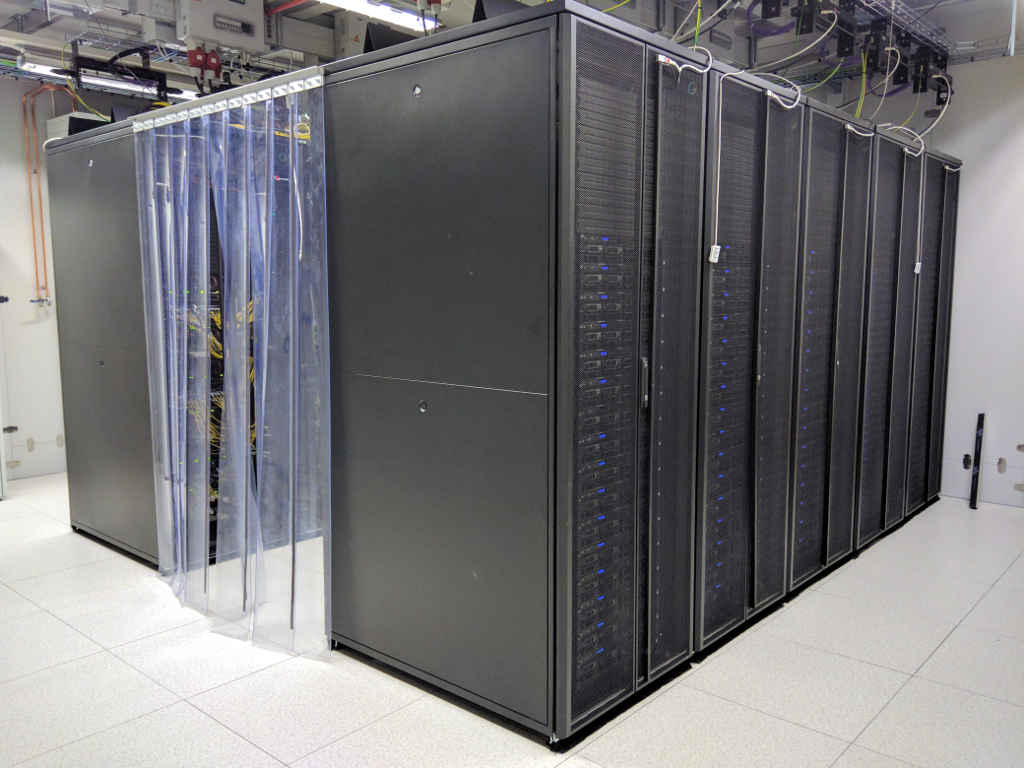
\includegraphics[width=1.0\linewidth]{pod2_interior.jpg}
\end{tiny}
\caption{Server racks in data center module POD 2 at RISE SICS North.}
\end{figure}
\end{column}%
\end{columns}
\end{frame}

%%%%%%%%%%%%%%%%%%%%%%%%%%%%%%%%%%%%%%%%%%%%%%%%%%%%%%%%%%%%%%%%%%%%%%%%
\begin{frame}{Data Centers}
\begin{columns}[T]% align columns
\begin{column}{.5\textwidth}
\begin{figure}[ht]
\begin{center}
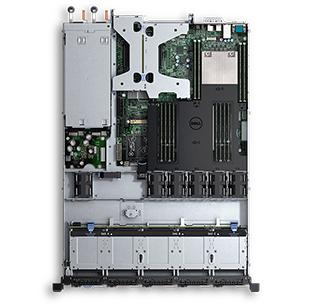
\includegraphics[width=1.2\linewidth]{dell_r430.jpg}
\end{center}
\caption{Dell R430 blade server with six internal fans.}
\end{figure}
\end{column}%
\hfill%
\begin{column}{.5\textwidth}
\begin{figure}[ht]
\begin{center}
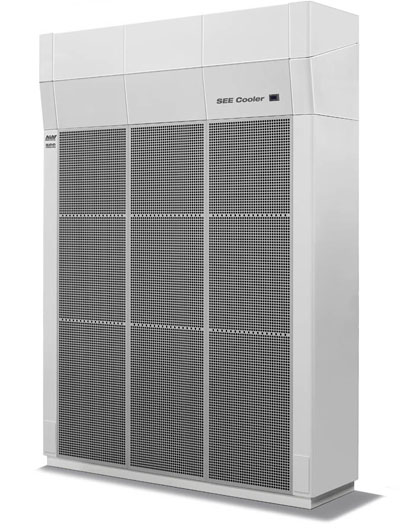
\includegraphics[width=0.95\linewidth]{crac.jpg}
\end{center}
\caption{Computer Room Air Conditioner, SEE Cooler HDZ-3.}
\end{figure}
\end{column}%
\end{columns}
\end{frame}

%%%%%%%%%%%%%%%%%%%%%%%%%%%%%%%%%%%%%%%%%%%%%%%%%%%%%%%%%%%%%%%%%%%%%%%%
\begin{frame}{Data Centers}
\begin{figure}[!htb]
\centering
\begin{tiny} % For text embedded in figure
\def\svgwidth{0.85\linewidth}
\input{Figures/flow.pdf_tex}
\end{tiny}
\caption{Theoretical heat flow in the data center POD 2 at RISE SICS North. Hot aisle configuration.}
\label{fig:flow}
\end{figure}
\end{frame}

%%%%%%%%%%%%%%%%%%%%%%%%%%%%%%%%%%%%%%%%%%%%%%%%%%%%%%%%%%%%%%%%%%%%%%%%
\begin{frame}{Data Centers}
\begin{itemize}
\item The full Information Communication
Technology (ICT) electrical energy footprint was estimated to be 900TWh in
2012, corresponding to 4.6\% of the total global electricity
consumption\footnotemark.
\item In a 2017 study of 100 data centers, air conditioning systems were often found ineffective using between 21 to 61\% of the total facility energy, averaging at 38\%\footnotemark.
\item How to achieve the most energy efficient cooling while meeting thermal specifications?
\item Computational Fluid Dynamics (CFD) make it possible to test different cooling control systems and configurations.
\end{itemize}
\footnotetext[1]{W. Van Heddeghem, S. Lambert, B. Lannoo, D. Colle, M. Pickavet, and P. Demeester, “Trends in worldwide ICT electricity consumption from 2007 to 2012,” Comput. Commun., vol. 50, pp. 6476, Sep. 2014.}
\footnotetext[2]{J. Ni and X. Bai, “A review of air conditioning energy performance in data centers,” Renew. Sustain. Energy Rev., vol. 67, pp. 625640, Jan.
2017.}
\end{frame}

\subsection{Fluid Dynamics}
%%%%%%%%%%%%%%%%%%%%%%%%%%%%%%%%%%%%%%%%%%%%%%%%%%%%%%%%%%%%%%%%%%%%%%%%
\begin{frame}{Fluid Dynamics}
The most common equation in fluid dynamics is the Navier-Stokes equation. For compressible fluids
\begin{equation}
\rho \left( \frac{\partial \vec{u}}{\partial t} + (\vec{u} \cdot \nabla) \vec{u} \right)
=
- \nabla \vec{p}
+ \rho g
+ \mu \nabla^2 \vec{u},
\end{equation}
which represent the conservation of linear momentum and pressure. It is most often used with the continuity equation
\begin{equation}
\frac{\partial \rho}{\partial t} + \nabla \cdot (\rho \vec{u}) = 0.
\end{equation}
representing the conservation of mass.
\end{frame}

\subsection{Computational Fluid Dynamics}
%%%%%%%%%%%%%%%%%%%%%%%%%%%%%%%%%%%%%%%%%%%%%%%%%%%%%%%%%%%%%%%%%%%%%%%%
\begin{frame}{Computational Fluid Dynamics (CFD)}
A physical fluid flow problem is stated using general sets of partial differential equations constrained by boundary conditions and initial conditions.
\begin{figure}[H]
\centering
\begin{tiny}
\def\svgwidth{1.0\linewidth}
\input{Figures/ibvp.pdf_tex}
\end{tiny}
\caption{The Initial Boundary Value Problem.}
\label{fig:ibvp}
\end{figure}
\end{frame}

%%%%%%%%%%%%%%%%%%%%%%%%%%%%%%%%%%%%%%%%%%%%%%%%%%%%%%%%%%%%%%%%%%%%%%%%
\begin{frame}{Commercial and Open Source CFD toolkits}
\begin{columns}[T] % align columns
\begin{column}{.6\textwidth}
FEM and FVM methods are based on the Navier-Stokes equations and the continuity equation.

Models fluid behavior as a continuum, but discretizes domain into finite volumes/elements.

Examples:

\begin{itemize}
\item ANSYS CFX (FVM \& FEM)
\item COMSOL Multiphysics (FEM)
\item OpenFOAM (FVM)
\end{itemize}
\end{column}%
\begin{column}{.5\textwidth}
\begin{figure}[!htb]
\centering
\begin{tiny} % For text embedded in figure
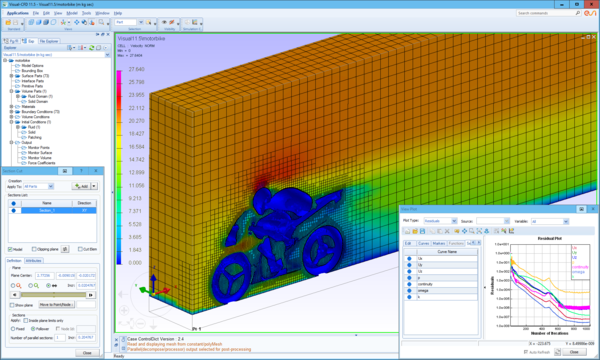
\includegraphics[width=1.0\linewidth]{visual-cfd.png}
\end{tiny}
\caption{GUI for OpenFOAM called Visual-CFD.}
\end{figure}
\end{column}%
\end{columns}

\end{frame}

\section{The Lattice Boltzmann Method (LBM)}
%%%%%%%%%%%%%%%%%%%%%%%%%%%%%%%%%%%%%%%%%%%%%%%%%%%%%%%%%%%%%%%%%%%%%%%%
\begin{frame}{The Lattice Boltzmann Method (LBM)}
The LBM models the behavior of a group of particles as distribution functions in a uniform grid.
\begin{figure}[H]
\centering
\begin{scriptsize}
\def\svgwidth{\linewidth}
\input{Figures/scales.pdf_tex}
\end{scriptsize}
\caption{Techniques of simulations for different scales of fluid representations.}
\label{fig:scales}
\end{figure}
\end{frame}

%%%%%%%%%%%%%%%%%%%%%%%%%%%%%%%%%%%%%%%%%%%%%%%%%%%%%%%%%%%%%%%%%%%%%%%%
\begin{frame}{LBM: Space Discretization}
LBM discretizes the domain into a uniform grid of cells called lattice sites.
\begin{figure}[!htb]
\centering
\begin{minipage}[t]{.45\textwidth}
	\centering
	\begin{tiny}
	\def\svgwidth{0.9\linewidth}
	\input{Figures/d3q19.pdf_tex}
	\end{tiny}
	\caption{D3Q19 lattice site.}
	\label{fig:d2q9_1}
\end{minipage}\qquad%
\begin{minipage}[t]{.45\textwidth}
	\centering
	\begin{tiny}
	\def\svgwidth{0.9\linewidth}
	\input{Figures/d2q9_2.pdf_tex}
	\end{tiny}
	\caption{D2Q9 lattice site. Direction vectors $\vec{e}_i$ are lattice velocities, with their corresponding weight $w_i$.}
	\label{fig:d2q9_2}
\end{minipage}
\end{figure}
\end{frame}

%%%%%%%%%%%%%%%%%%%%%%%%%%%%%%%%%%%%%%%%%%%%%%%%%%%%%%%%%%%%%%%%%%%%%%%%
\begin{frame}{The Boltzmann Equation}
The Boltzmann equation is based on a concept called \textit{kinetic theory}. Velocity distribution function
\begin{equation}
f^{(N)}(\vec{x}^{(N)}, \vec{p}^{(N)}, t)
\end{equation}
gives the probability of finding $N$ number of particles with the displacements $\vec{x}$ and momentums $\vec{p}$ at the time $t$. For non-dilute gases $f^{(1)}$ is sufficient.

If disturbed by external force future positions and momentums are
\begin{equation}
f^{(1)}(\vec{x}+\Delta \vec{x}, \vec{p}+\Delta \vec{p}, t+\Delta t),
\end{equation}
if no particle collisions take place.
\end{frame}

%%%%%%%%%%%%%%%%%%%%%%%%%%%%%%%%%%%%%%%%%%%%%%%%%%%%%%%%%%%%%%%%%%%%%%%%
\begin{frame}{The Boltzmann Equation}
When taking particle collisions into account however,
\begin{equation} \label{eq:be}
\left( \vec{u}\cdot\nabla_{\vec{x}} +F\cdot\nabla_{\vec{p}} + \frac{\partial}{\partial t} \right) f^{(1)}(\vec{x}, \vec{p}, t) = \Gamma^{(+)} - \Gamma^{(-)}.
\end{equation}
$\Gamma^{(-)}$ represents the number of particles starting at $(\vec{x},~\vec{p})$ and not arriving at $(\vec{x}+\Delta\vec{x},~\vec{p}+\Delta\vec{p})$ due to particle collisions. Vice versa for $\Gamma^{(+)}$.
\end{frame}

%%%%%%%%%%%%%%%%%%%%%%%%%%%%%%%%%%%%%%%%%%%%%%%%%%%%%%%%%%%%%%%%%%%%%%%%
\begin{frame}{LBM: The Discrete Lattice Boltzmann Equation}
The evolution of the system is described by the Discrete Lattice Boltzmann Equation
\begin{equation} \label{eq:dbe}
f_i(\vec{x} + \vec{e_i}\Delta t, t + \Delta t) = f_i(\vec{x}, t) + \Gamma(f_i(\vec{x}, t)).
\end{equation}
Each distribution function $f_i$ is associated with a direction.

$\Gamma$ is called a collision operator and can be implemented in different ways. RAFSINE uses the Bhatnagar--Gross--Krook (BGK) method.

\end{frame}

%%%%%%%%%%%%%%%%%%%%%%%%%%%%%%%%%%%%%%%%%%%%%%%%%%%%%%%%%%%%%%%%%%%%%%%%%
%\begin{frame}{LBM: Bhatnagar, Gross and Krook (BGK)}
%The BGK implements the collision operator $\Gamma(f_i(\vec{x}, t))$ by
%\begin{equation}\label{eq:bgk}
%f_i(\vec{x}+\vec{e}_i \Delta t, t+\Delta t) = f_i(\vec{x},t) - \frac{1}{\tau} \left( f_i(\vec{x},t)-f_i^{eq}(\vec{x},t) \right),
%\end{equation}
%using relaxation towards a local equilibrium function
%\begin{equation}
%f_i^{eq}(\vec{x}) = w_i \rho(\vec{x}) \left(1 + \frac{\vec{e}_i \cdot \vec{u}}{c_s^2} + \frac{(\vec{e}_i \cdot \vec{u})^2}{2c_s^4} - \frac{\vec{u}^2}{2c_s^2} \right),
%\end{equation}
%where $c_s$ is a basic lattice speed. Relaxation time $\tau$ is related to kinematic viscosity
%$\nu=\frac{1}{3}\left(\tau-\frac{1}{2}\right).$
%\end{frame}

%%%%%%%%%%%%%%%%%%%%%%%%%%%%%%%%%%%%%%%%%%%%%%%%%%%%%%%%%%%%%%%%%%%%%%%%%
%\begin{frame}{LBM: Bhatnagar, Gross and Krook (BGK)}
%Particle density and momentum
%\begin{align}
%\rho &= \sum\limits_{i}^{} f_i,\\
%\vec{p} &= \rho\vec{u} = \sum\limits_{i}^{} f_i \vec{e_i}.
%\end{align}
%Temperature $T$ of a lattice site can be calculated as second order moment
%\begin{align}
%\rho e &= \frac{1}{2} \sum\limits_{i}^{} (\vec{e}_i-\vec{u})^2 f_i,\\
%e &= \frac{3k}{2mT}
%\end{align}
%where $e$ is internal energy, $k$ is called \textit{Boltzmann factor} and $m$ is mass, but this is inaccurate because of discretization errors. 
%\end{frame}

%%%%%%%%%%%%%%%%%%%%%%%%%%%%%%%%%%%%%%%%%%%%%%%%%%%%%%%%%%%%%%%%%%%%%%%%%
%\begin{frame}{LBM: Bhatnagar, Gross and Krook (BGK)}
%An independent set of \textit{temperature distribution functions} are used on a D3Q6 lattice, with evolution
%\begin{equation}
%T_i(\vec{x}+\vec{e}_i \Delta t, t+\Delta t) = T_i(\vec{x},t) - \frac{1}{\tau_T} \left( T_i(\vec{x},t)-T_i^{eq}(\vec{x},t) \right),
%\end{equation}
%and equilibrium function
%\begin{equation}
%T_i^{eq}(\vec{x}) = \frac{T}{b} \left( 1+\frac{b}{2}\vec{e}_i \cdot \vec{u} \right),
%\end{equation}
%where $b=7$ for a D3Q6 lattice. Relaxation time $\tau_T$ is related to thermal diffusivity
%\begin{equation}
%\alpha = \frac{2\tau_T - 1}{4}\cdot\frac{\Delta x^2}{\Delta t}.
%\end{equation}
%Temperature of a site can be recovered as $T = \sum\limits_{i}^{} T_i$.
%\end{frame}

\begin{frame}{LBM: Bhatnagar, Gross and Krook (BGK)}
The BGK implements the collision operator $\Gamma(f_i(\vec{x}, t))$ for velocity distribution functions
\begin{equation}\label{eq:bgk}
f_i(\vec{x}+\vec{e}_i \Delta t, t+\Delta t) = f_i(\vec{x},t) - \frac{1}{\tau} \left( f_i(\vec{x},t)-f_i^{eq}(\vec{x},t) \right)
\end{equation}
and temperature distribution functions
\begin{equation}\label{eq:bgk_t}
T_i(\vec{x}+\vec{e}_i \Delta t, t+\Delta t) = T_i(\vec{x},t) - \frac{1}{\tau_T} \left( T_i(\vec{x},t)-T_i^{eq}(\vec{x},t) \right).
\end{equation}
\end{frame}

%%%%%%%%%%%%%%%%%%%%%%%%%%%%%%%%%%%%%%%%%%%%%%%%%%%%%%%%%%%%%%%%%%%%%%%%
\begin{frame}{LBM: Natural Convection}
\begin{columns}[T] % align columns
\begin{column}{.5\textwidth}
Buoyancy by Boussinesq approximation ignores density differences
\begin{equation}
\vec{F}_B = -\vec{g}\beta(T-T_0),
\end{equation}
$\vec{g}$ gravity vector,

$(T-T_0)$ thermal gradient,

$\beta$ thermal expansion coefficient at reference temperature $T_0$.

\end{column}%
\hfill%
\begin{column}{0.4\textwidth}
\begin{figure}[t]
	\begin{tiny}
	\def\svgwidth{1.0\linewidth}
	\input{Figures/natural_convection.pdf_tex}
	\end{tiny}
\caption{Flow due to natural convection.}
\label{fig:natural_convection}
\end{figure}
\end{column}%
\end{columns}
%\hskip -10pt
%Added to up/down velocity distribution functions:
%\begin{footnotesize}
%\begin{align}
%f_5(\vec{x}, t+\Delta t) &= f_5^{temp}(\vec{x},t) - \frac{f_5^{temp}(\vec{x},t)-f_5^{eq}(\vec{x},t)}{\tau} + \frac{\vec{g}\beta(T-T_0)}{2}\\
%f_6(\vec{x}, t+\Delta t) &= f_6^{temp}(\vec{x},t) - \frac{f_6^{temp}(\vec{x},t)-f_6^{eq}(\vec{x},t)}{\tau} - \frac{\vec{g}\beta(T-T_0)}{2}
%\end{align}
%\end{footnotesize}
\end{frame}

%%%%%%%%%%%%%%%%%%%%%%%%%%%%%%%%%%%%%%%%%%%%%%%%%%%%%%%%%%%%%%%%%%%%%%%%%
%\begin{frame}{LBM: Turbulence}
%\begin{columns}[T] % align columns
%\begin{column}{.5\textwidth}
%\begin{itemize}
%\item \textit{Laminar} flows, all parts move in a uniform fashion, shear stress proportional to velocity.
%\item Increased shear stress makes the flow \textit{turbulent}.
%\item Magnitude of turbulence is defined by the Reynolds number
%\end{itemize}
%\begin{equation}
%\textrm{Re} = \frac{\vec{U} \ell}{\nu} = \frac{\vec{U}_{lbm} N}{\nu_{lbm}}.
%\end{equation}
%\hfill%
%\end{column}%
%\begin{column}{0.5\textwidth}
%\begin{figure}[H]
%\centering
%\begin{scriptsize}
%\def\svgwidth{1.0\linewidth}
%\input{Figures/reynold.pdf_tex}
%\end{scriptsize}
%\caption{Flow conditions for different Reynolds numbers.}
%\label{fig:reynold}
%\end{figure}
%\end{column}%
%\end{columns}
%\end{frame}

%%%%%%%%%%%%%%%%%%%%%%%%%%%%%%%%%%%%%%%%%%%%%%%%%%%%%%%%%%%%%%%%%%%%%%%%
\begin{frame}{LBM: Turbulence}
\begin{figure}[H]
\centering
\begin{scriptsize}
\def\svgwidth{0.5\linewidth}
\input{Figures/reynold.pdf_tex}
\end{scriptsize}
\caption{Flow conditions for different Reynolds numbers.}
\label{fig:reynold}
\end{figure}

Large Eddy Simulation (LES) ignores dynamics of small scale swirling motion of fluids (eddies) since large scale eddies carry more energy. Based on applying a low-pass filter on the Navier-Stokes equations.

%Local momentum stress tensor defines the flux of the $\alpha$th component of the momentum vector $\vec{u}_{\alpha}$ across a surface with the constant coordinate $x_{\beta}$
%\begin{equation}
%\bar{S}_{\alpha \beta}
%=
%\frac{1}{2} \left(
%\frac{\partial \vec{u}_{\alpha}}{\partial x_{\beta}}
%+
%\frac{\partial \vec{u}_{\beta}}{\partial x_{\alpha}}
%\right)
%=
%\sum\limits_{i=1}^{q} \vec{e}_{i\alpha} \vec{e}_{i\beta} \left( f_i - f^{eq}_i \right).
%\end{equation}
\end{frame}
%
%%%%%%%%%%%%%%%%%%%%%%%%%%%%%%%%%%%%%%%%%%%%%%%%%%%%%%%%%%%%%%%%%%%%%%%%%
%\begin{frame}{LBM: Turbulence}
%Eddy viscosity, where $C_S > 0$ is called the \textit{Smagorinsky constant},
%\begin{equation}
%\nu_t = \frac{1}{6} \left( \sqrt{\nu^2 + 18 C_S^2 (\Delta x)^2 \sqrt{\bar{S}_{\alpha \beta}\bar{S}_{\alpha \beta}}} \right),
%\end{equation}
%is inputted into relaxation time along with kinematic viscosity $\nu_0$,
%\begin{equation}
%\tau = \frac{1}{2}+3(\nu_0+\nu_t).
%\end{equation}

%\end{frame}

%%%%%%%%%%%%%%%%%%%%%%%%%%%%%%%%%%%%%%%%%%%%%%%%%%%%%%%%%%%%%%%%%%%%%%%%
\begin{frame}{LBM: Initialization Step}
At time $t=0$ the distribution functions are initialized
\begin{equation}
f_i(\vec{x},0) = f_i^{eq} (\rho (\vec{x}), \vec{u} (\vec{x})),
\end{equation}
where $\rho$ is the initial pressure and $\vec{u}$ is initial velocity.
\end{frame}

%%%%%%%%%%%%%%%%%%%%%%%%%%%%%%%%%%%%%%%%%%%%%%%%%%%%%%%%%%%%%%%%%%%%%%%%
\begin{frame}{LBM: Streaming Step}
\begin{figure}[!htb]
\centering
\begin{minipage}[t]{.45\textwidth}
	\centering
	\begin{small}
	\def\svgwidth{0.9\linewidth}
	\input{Figures/d2q9_3.pdf_tex}
	\end{small}
	\caption{Lattice streaming step, representing advection in a fluid. All functions $f_i$ are copied to the neighboring $f_i^{temp}$ in parallel.}
	\label{fig:d2q9_3}
\end{minipage}\qquad%
\begin{minipage}[t]{.45\textwidth}
	\centering
	\begin{small}
	\def\svgwidth{0.9\linewidth}
	\input{Figures/d2q9_4.pdf_tex}
	\end{small}
	\caption{Also in the streaming step, the current site is filled with new distributions from the neighboring sites.}
	\label{fig:d2q9_4}
\end{minipage}
\end{figure}
\end{frame}

%%%%%%%%%%%%%%%%%%%%%%%%%%%%%%%%%%%%%%%%%%%%%%%%%%%%%%%%%%%%%%%%%%%%%%%%
\begin{frame}{LBM: Collision Step}
\begin{figure}[!htb]
\centering
\begin{minipage}[t]{.45\textwidth}
	\centering
	\begin{footnotesize}
	\def\svgwidth{0.9\linewidth}
	\input{Figures/d2q9_5.pdf_tex}
	\end{footnotesize}
	\caption{Collision step, representing diffusion in a fluid. Particles from adjacent sites collide locally in the current site (see BGK).}
	\label{fig:d2q9_5}
\end{minipage}\qquad%
\begin{minipage}[t]{.45\textwidth}
	\centering
	\begin{small}
	\def\svgwidth{0.9\linewidth}
	\input{Figures/d2q9_6.pdf_tex}
	\end{small}
	\caption{During the collide step the particle populations are redistributed. Both mass and momentum is conserved.}
	\label{fig:d2q9_6}
\end{minipage}
\end{figure}
\end{frame}

%%%%%%%%%%%%%%%%%%%%%%%%%%%%%%%%%%%%%%%%%%%%%%%%%%%%%%%%%%%%%%%%%%%%%%%%
\begin{frame}{LBM: Boundary Step}
\begin{columns}[T] % align columns
\begin{column}{.7\textwidth}
Boundary conditions define what happens at the edges of the domain.

Dirichlet specifies solution by value, e.g.

\begin{itemize}
\item Periodic (infinity)
\item No-slip condition (walls)
\end{itemize}

Von Neumann specifies the derivative of a solution, e.g.

\begin{itemize}
\item Zero-gradient \mbox{(fan intake)}
\item Node-to-node velocity increase \mbox{(fan exhaust)}
\end{itemize}
\end{column}%
\hfill%
\begin{column}{0.3\textwidth}
\begin{figure}[t]
	\begin{tiny}
	\def\svgwidth{0.9\linewidth}
	\input{Figures/bounce-back-hw.pdf_tex}
	\end{tiny}
	\caption{Half-way bounce-back boundary condition on a D2Q9 lattice.}
	\label{fig:bounce-back-hw}
\end{figure}
\end{column}%
\end{columns}
\end{frame}

\section{RAFSINE}
%%%%%%%%%%%%%%%%%%%%%%%%%%%%%%%%%%%%%%%%%%%%%%%%%%%%%%%%%%%%%%%%%%%%%%%%
\begin{frame}{RAFSINE}

\begin{itemize}
\item Written by Nicolas Delbosc during his Ph.D study in the School of Mechanical Engineering at the
University of Leeds, England.
\item Implements LBM (BGK model) in C++ with streaming-, collision- and boundary-steps accelerated by Nvidia CUDA.
\item Simulates fluid behavior in real time or faster depending on domain size.
\item OpenGL visualization of system evolution.
\end{itemize}

\begin{figure}[ht]
\begin{center}
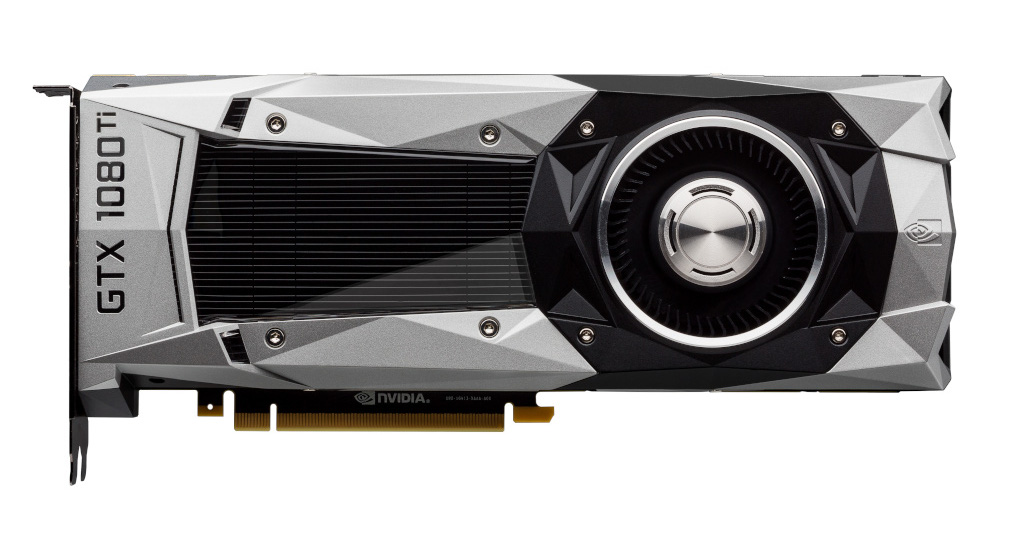
\includegraphics[width=0.5\linewidth]{1080ti.jpg}
\end{center}
\caption{Nvidia GTX 1080 Ti.}
\end{figure}

\end{frame}

%%%%%%%%%%%%%%%%%%%%%%%%%%%%%%%%%%%%%%%%%%%%%%%%%%%%%%%%%%%%%%%%%%%%%%%%
\begin{frame}{RAFSINE}

\begin{figure}[ht]
\begin{center}
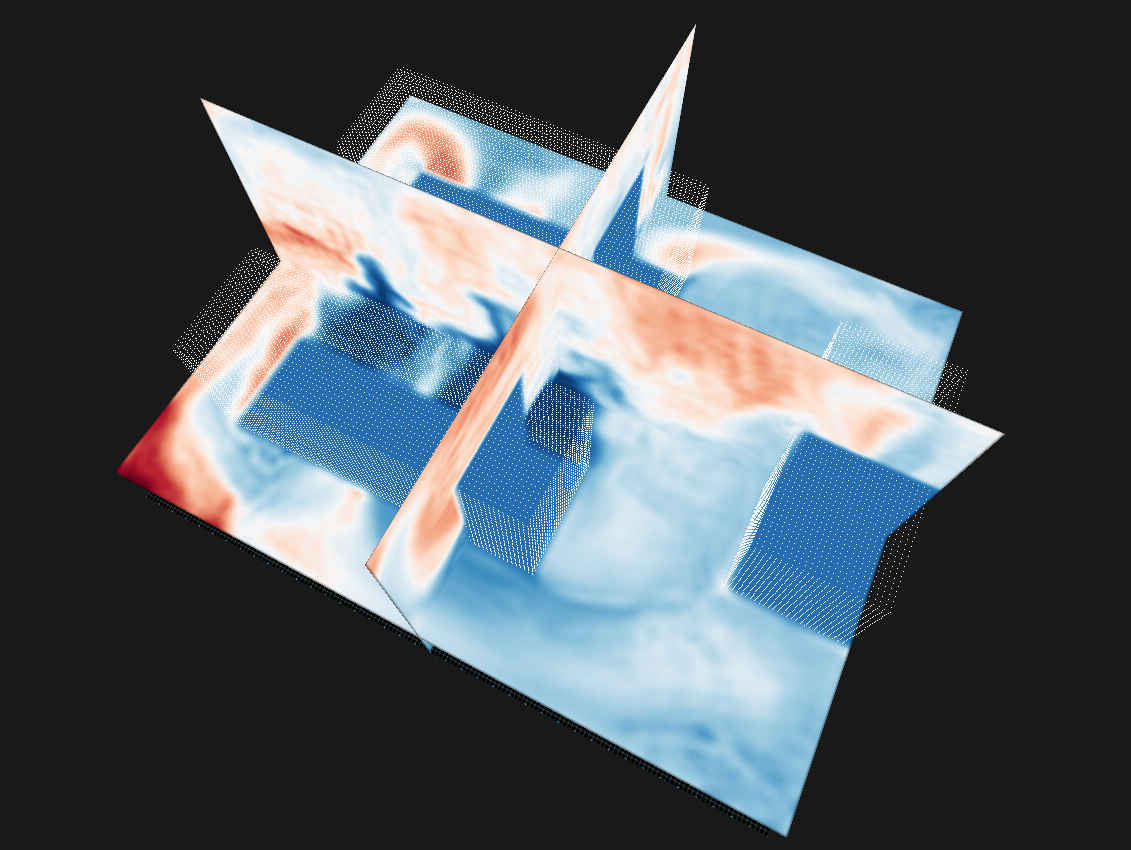
\includegraphics[width=0.9\linewidth]{rafsine_problem1.jpg}
\end{center}
\caption{Visualization of heat flow in a data center with cold aisle.}
\label{fig:problem2}
\end{figure}

\end{frame}


%%%%%%%%%%%%%%%%%%%%%%%%%%%%%%%%%%%%%%%%%%%%%%%%%%%%%%%%%%%%%%%%%%%%%%%%
\begin{frame}{RAFSINE}
\begin{figure}[!htb]
\centering
\begin{scriptsize}
\def\svgwidth{0.7\linewidth}
\input{Figures/lbm-core.pdf_tex}
\end{scriptsize}
\caption{Structure of the LBM program.}
\label{fig:lbm-core}
\end{figure}
How to use the OpenGL visualization of a headless server on a local workstation?
\end{frame}

\section{Deployment}
\subsection{VirtualGL}
%%%%%%%%%%%%%%%%%%%%%%%%%%%%%%%%%%%%%%%%%%%%%%%%%%%%%%%%%%%%%%%%%%%%%%%%
\begin{frame}{VirtualGL: OpenGL over VNC}
\begin{figure}[!htb]
\centering
\begin{scriptsize}
\def\svgwidth{0.7\linewidth}
\input{Figures/virtualgl_direct.pdf_tex}
\end{scriptsize}
\caption{Direct OpenGL rendering using GLX on a local GPU with a monitor attached.}
\label{fig:virtualgl_direct}
\end{figure}
\end{frame}

%%%%%%%%%%%%%%%%%%%%%%%%%%%%%%%%%%%%%%%%%%%%%%%%%%%%%%%%%%%%%%%%%%%%%%%%
\begin{frame}{VirtualGL: OpenGL over VNC}
\begin{figure}[!htb]
\centering
\begin{scriptsize}
\def\svgwidth{0.9\linewidth}
\input{Figures/virtualgl_forking.pdf_tex}
\end{scriptsize}
\caption{In-Process GLX Forking with an X11 proxy over a network, in the form of a VNC server and client.}
\label{fig:virtualgl_forking}
\end{figure}
\end{frame}

\subsection{Multithreading}
%%%%%%%%%%%%%%%%%%%%%%%%%%%%%%%%%%%%%%%%%%%%%%%%%%%%%%%%%%%%%%%%%%%%%%%%
\begin{frame}{Improving performance}
Original code was mostly sequential, rendering the simulation blocked execution. Problematic with VirtualGL.
\begin{figure}[!htb]
\hspace*{-0.3in}
\centering
\begin{tiny}
\def\svgwidth{1.1\linewidth}
\input{Figures/singlethreading.pdf_tex}
\end{tiny}
\caption{Single threading in the original RAFSINE application.}
\label{fig:singlethreading}
\end{figure}
\end{frame}

%%%%%%%%%%%%%%%%%%%%%%%%%%%%%%%%%%%%%%%%%%%%%%%%%%%%%%%%%%%%%%%%%%%%%%%%
\begin{frame}{Improving performance}
\begin{figure}[!htb]
\hspace*{-0.3in}
\centering
\begin{tiny}
\def\svgwidth{1.1\linewidth}
%LaTeX with PSTricks extensions
%%Creator: inkscape 0.92.2
%%Please note this file requires PSTricks extensions
\psset{xunit=.5pt,yunit=.5pt,runit=.5pt}
\begin{pspicture}(787.32000732,266.38665771)
{
\newrgbcolor{curcolor}{0.94117647 0.94117647 0.94117647}
\pscustom[linestyle=none,fillstyle=solid,fillcolor=curcolor]
{
\newpath
\moveto(5.19530654,70.91825261)
\lineto(5.19530654,3.93957428)
\lineto(784.79998038,3.93957428)
\lineto(784.79998038,137.89598427)
\lineto(5.19530654,137.89598427)
}
}
{
\newrgbcolor{curcolor}{0.69411767 0.69411767 0.69411767}
\pscustom[linewidth=0.15108666,linecolor=curcolor]
{
\newpath
\moveto(5.19530654,70.91825261)
\lineto(5.19530654,3.93957428)
\lineto(784.79998038,3.93957428)
\lineto(784.79998038,137.89598427)
\lineto(5.19530654,137.89598427)
\closepath
}
}
{
\newrgbcolor{curcolor}{0.87843138 0.87843138 0.87843138}
\pscustom[linestyle=none,fillstyle=solid,fillcolor=curcolor]
{
\newpath
\moveto(5.19530654,199.42131606)
\lineto(5.19530654,136.22265098)
\lineto(784.79998038,136.22265098)
\lineto(784.79998038,262.61998115)
\lineto(5.19530654,262.61998115)
}
}
{
\newrgbcolor{curcolor}{0.69411767 0.69411767 0.69411767}
\pscustom[linewidth=0.15108666,linecolor=curcolor]
{
\newpath
\moveto(5.19530654,199.42131606)
\lineto(5.19530654,136.22265098)
\lineto(784.79998038,136.22265098)
\lineto(784.79998038,262.61998115)
\lineto(5.19530654,262.61998115)
\closepath
}
}
{
\newrgbcolor{curcolor}{0 0 0}
\pscustom[linewidth=1.51154667,linecolor=curcolor]
{
\newpath
\moveto(754.24798114,21.32812051)
\lineto(100.39013082,21.32812051)
}
}
{
\newrgbcolor{curcolor}{0 0 0}
\pscustom[linewidth=1.51154667,linecolor=curcolor]
{
\newpath
\moveto(754.24798114,112.03638491)
\lineto(100.39013082,112.03638491)
}
}
{
\newrgbcolor{curcolor}{0 0 0}
\pscustom[linewidth=1.51154667,linecolor=curcolor]
{
\newpath
\moveto(754.24798114,66.68225271)
\lineto(100.39013082,66.68225271)
}
}
{
\newrgbcolor{curcolor}{0.99607843 0.99607843 0.99607843}
\pscustom[linestyle=none,fillstyle=solid,fillcolor=curcolor]
{
\newpath
\moveto(111.79733054,68.05625268)
\lineto(111.79733054,58.04638626)
\lineto(182.43999544,58.04638626)
\lineto(182.43999544,78.06665243)
\lineto(111.79733054,78.06665243)
}
}
{
\newrgbcolor{curcolor}{0 0 0}
\pscustom[linewidth=1.51154667,linecolor=curcolor]
{
\newpath
\moveto(111.79733054,68.05625268)
\lineto(111.79733054,58.04638626)
\lineto(182.43999544,58.04638626)
\lineto(182.43999544,78.06665243)
\lineto(111.79733054,78.06665243)
\closepath
}
}
{
\newrgbcolor{curcolor}{0 0 0}
\pscustom[linestyle=none,fillstyle=solid,fillcolor=curcolor]
{
\newpath
\moveto(135.40208744,71.8404896)
\lineto(135.40208744,70.45895169)
\curveto(134.96103308,70.86973761)(134.48971029,71.17674604)(133.98811907,71.37997697)
\curveto(133.4908519,71.58320789)(132.96115427,71.68482336)(132.39902617,71.68482336)
\curveto(131.29206622,71.68482336)(130.44455,71.34538447)(129.85647753,70.66650668)
\curveto(129.26840506,69.99195296)(128.97436882,69.01471488)(128.97436882,67.73479244)
\curveto(128.97436882,66.45919406)(129.26840506,65.48195598)(129.85647753,64.80307819)
\curveto(130.44455,64.12852447)(131.29206622,63.79124761)(132.39902617,63.79124761)
\curveto(132.96115427,63.79124761)(133.4908519,63.89286308)(133.98811907,64.09609401)
\curveto(134.48971029,64.29932493)(134.96103308,64.60633336)(135.40208744,65.01711928)
\lineto(135.40208744,63.64855356)
\curveto(134.94373684,63.33722107)(134.45727983,63.10372171)(133.94271641,62.94805546)
\curveto(133.43247706,62.79238922)(132.89196927,62.7145561)(132.32119305,62.7145561)
\curveto(130.85533592,62.7145561)(129.70081129,63.16209655)(128.85761914,64.05717745)
\curveto(128.01442699,64.95658241)(127.59283091,66.18245407)(127.59283091,67.73479244)
\curveto(127.59283091,69.29145487)(128.01442699,70.51732653)(128.85761914,71.41240743)
\curveto(129.70081129,72.31181239)(130.85533592,72.76151487)(132.32119305,72.76151487)
\curveto(132.90061739,72.76151487)(133.44544925,72.68368175)(133.9556886,72.52801551)
\curveto(134.47025201,72.37667333)(134.95238496,72.14749803)(135.40208744,71.8404896)
\closepath
}
}
{
\newrgbcolor{curcolor}{0 0 0}
\pscustom[linestyle=none,fillstyle=solid,fillcolor=curcolor]
{
\newpath
\moveto(137.60145748,72.58639035)
\lineto(138.91813446,72.58639035)
\lineto(138.91813446,66.70350358)
\curveto(138.91813446,65.66572862)(139.10623117,64.91766584)(139.48242459,64.45931524)
\curveto(139.85861801,64.0052887)(140.46831079,63.77827543)(141.31150294,63.77827543)
\curveto(142.15037103,63.77827543)(142.75790179,64.0052887)(143.13409521,64.45931524)
\curveto(143.51028863,64.91766584)(143.69838534,65.66572862)(143.69838534,66.70350358)
\lineto(143.69838534,72.58639035)
\lineto(145.01506231,72.58639035)
\lineto(145.01506231,66.54135124)
\curveto(145.01506231,65.27872505)(144.70156779,64.32526931)(144.07457876,63.68098402)
\curveto(143.45191379,63.03669874)(142.53088852,62.7145561)(141.31150294,62.7145561)
\curveto(140.08779331,62.7145561)(139.16244398,63.03669874)(138.53545494,63.68098402)
\curveto(137.91278997,64.32526931)(137.60145748,65.27872505)(137.60145748,66.54135124)
\closepath
}
}
{
\newrgbcolor{curcolor}{0 0 0}
\pscustom[linestyle=none,fillstyle=solid,fillcolor=curcolor]
{
\newpath
\moveto(148.9808258,71.50969883)
\lineto(148.9808258,63.97934432)
\lineto(150.5634326,63.97934432)
\curveto(151.89956786,63.97934432)(152.87680594,64.28202869)(153.49514685,64.88739741)
\curveto(154.11781182,65.49276613)(154.42914431,66.4483839)(154.42914431,67.75425072)
\curveto(154.42914431,69.05146941)(154.11781182,70.00060109)(153.49514685,70.60164575)
\curveto(152.87680594,71.20701447)(151.89956786,71.50969883)(150.5634326,71.50969883)
\closepath
\moveto(147.67063492,72.58639035)
\lineto(150.36236371,72.58639035)
\curveto(152.23900675,72.58639035)(153.61622059,72.19506271)(154.49400524,71.41240743)
\curveto(155.37178989,70.63407622)(155.81068221,69.41469065)(155.81068221,67.75425072)
\curveto(155.81068221,66.08516267)(155.36962786,64.859291)(154.48751915,64.07663573)
\curveto(153.60541044,63.29398045)(152.23035862,62.90265281)(150.36236371,62.90265281)
\lineto(147.67063492,62.90265281)
\closepath
}
}
{
\newrgbcolor{curcolor}{0 0 0}
\pscustom[linestyle=none,fillstyle=solid,fillcolor=curcolor]
{
\newpath
\moveto(160.66740726,71.29565775)
\lineto(158.89021765,66.47649031)
\lineto(162.45108296,66.47649031)
\closepath
\moveto(159.9279926,72.58639035)
\lineto(161.41330801,72.58639035)
\lineto(165.10389519,62.90265281)
\lineto(163.74181556,62.90265281)
\lineto(162.85970685,65.38682661)
\lineto(158.49456595,65.38682661)
\lineto(157.61245724,62.90265281)
\lineto(156.23091933,62.90265281)
\closepath
}
}
{
\newrgbcolor{curcolor}{0.99607843 0.99607843 0.99607843}
\pscustom[linestyle=none,fillstyle=solid,fillcolor=curcolor]
{
\newpath
\moveto(274.31732648,22.70212048)
\lineto(274.31732648,12.69217406)
\lineto(401.65198996,12.69217406)
\lineto(401.65198996,32.71252023)
\lineto(274.31732648,32.71252023)
}
}
{
\newrgbcolor{curcolor}{0 0 0}
\pscustom[linewidth=1.51154667,linecolor=curcolor]
{
\newpath
\moveto(274.31732648,22.70212048)
\lineto(274.31732648,12.69217406)
\lineto(401.65198996,12.69217406)
\lineto(401.65198996,32.71252023)
\lineto(274.31732648,32.71252023)
\closepath
}
}
{
\newrgbcolor{curcolor}{0.99607843 0.99607843 0.99607843}
\pscustom[linestyle=none,fillstyle=solid,fillcolor=curcolor]
{
\newpath
\moveto(194.94666179,113.41091821)
\lineto(194.94666179,103.4010518)
\lineto(276.92799308,103.4010518)
\lineto(276.92799308,123.42078463)
\lineto(194.94666179,123.42078463)
}
}
{
\newrgbcolor{curcolor}{0 0 0}
\pscustom[linewidth=1.51154667,linecolor=curcolor]
{
\newpath
\moveto(194.94666179,113.41091821)
\lineto(194.94666179,103.4010518)
\lineto(276.92799308,103.4010518)
\lineto(276.92799308,123.42078463)
\lineto(194.94666179,123.42078463)
\closepath
}
}
{
\newrgbcolor{curcolor}{0 0 0}
\pscustom[linestyle=none,fillstyle=solid,fillcolor=curcolor]
{
\newpath
\moveto(205.05122394,115.64449773)
\lineto(205.05122394,108.11414322)
\lineto(206.63383074,108.11414322)
\curveto(207.969966,108.11414322)(208.94720408,108.41682758)(209.56554499,109.02219631)
\curveto(210.18820996,109.62756503)(210.49954245,110.5831828)(210.49954245,111.88904962)
\curveto(210.49954245,113.18626831)(210.18820996,114.13539999)(209.56554499,114.73644465)
\curveto(208.94720408,115.34181337)(207.969966,115.64449773)(206.63383074,115.64449773)
\closepath
\moveto(203.74103306,116.72118925)
\lineto(206.43276185,116.72118925)
\curveto(208.30940489,116.72118925)(209.68661873,116.32986161)(210.56440338,115.54720633)
\curveto(211.44218803,114.76887511)(211.88108035,113.54948954)(211.88108035,111.88904962)
\curveto(211.88108035,110.21996156)(211.440026,108.9940899)(210.55791729,108.21143462)
\curveto(209.67580858,107.42877934)(208.30075676,107.03745171)(206.43276185,107.03745171)
\lineto(203.74103306,107.03745171)
\closepath
}
}
{
\newrgbcolor{curcolor}{0 0 0}
\pscustom[linestyle=none,fillstyle=solid,fillcolor=curcolor]
{
\newpath
\moveto(214.94961681,116.36445411)
\lineto(214.94961681,114.30187638)
\lineto(217.40784623,114.30187638)
\lineto(217.40784623,113.37436502)
\lineto(214.94961681,113.37436502)
\lineto(214.94961681,109.43082019)
\curveto(214.94961681,108.83842366)(215.02961196,108.45790617)(215.18960227,108.28926774)
\curveto(215.35391663,108.12062931)(215.6847074,108.0363101)(216.18197457,108.0363101)
\lineto(217.40784623,108.0363101)
\lineto(217.40784623,107.03745171)
\lineto(216.18197457,107.03745171)
\curveto(215.26094929,107.03745171)(214.62531213,107.20825217)(214.27506309,107.54985309)
\curveto(213.92481404,107.89577807)(213.74968952,108.52276711)(213.74968952,109.43082019)
\lineto(213.74968952,113.37436502)
\lineto(212.8740669,113.37436502)
\lineto(212.8740669,114.30187638)
\lineto(213.74968952,114.30187638)
\lineto(213.74968952,116.36445411)
\closepath
}
}
{
\newrgbcolor{curcolor}{0 0 0}
\pscustom[linestyle=none,fillstyle=solid,fillcolor=curcolor]
{
\newpath
\moveto(221.70411689,113.46517033)
\curveto(221.06415566,113.46517033)(220.55824037,113.21437471)(220.18637102,112.71278349)
\curveto(219.81450166,112.21551632)(219.62856698,111.53231448)(219.62856698,110.66317795)
\curveto(219.62856698,109.79404143)(219.81233963,109.10867755)(220.17988492,108.60708632)
\curveto(220.55175428,108.10981916)(221.0598316,107.86118558)(221.70411689,107.86118558)
\curveto(222.33975405,107.86118558)(222.8435073,108.11198119)(223.21537666,108.61357242)
\curveto(223.58724602,109.11516364)(223.7731807,109.79836549)(223.7731807,110.66317795)
\curveto(223.7731807,111.52366635)(223.58724602,112.20470616)(223.21537666,112.70629739)
\curveto(222.8435073,113.21221268)(222.33975405,113.46517033)(221.70411689,113.46517033)
\closepath
\moveto(221.70411689,114.47700091)
\curveto(222.74189184,114.47700091)(223.55697759,114.13972405)(224.14937412,113.46517033)
\curveto(224.74177066,112.79061661)(225.03796893,111.85661915)(225.03796893,110.66317795)
\curveto(225.03796893,109.47406082)(224.74177066,108.54006336)(224.14937412,107.86118558)
\curveto(223.55697759,107.18663186)(222.74189184,106.849355)(221.70411689,106.849355)
\curveto(220.66201787,106.849355)(219.84477009,107.18663186)(219.25237356,107.86118558)
\curveto(218.66430108,108.54006336)(218.37026485,109.47406082)(218.37026485,110.66317795)
\curveto(218.37026485,111.85661915)(218.66430108,112.79061661)(219.25237356,113.46517033)
\curveto(219.84477009,114.13972405)(220.66201787,114.47700091)(221.70411689,114.47700091)
\closepath
}
}
{
\newrgbcolor{curcolor}{0 0 0}
\pscustom[linestyle=none,fillstyle=solid,fillcolor=curcolor]
{
\newpath
\moveto(226.97123173,115.64449773)
\lineto(226.97123173,108.11414322)
\lineto(228.55383854,108.11414322)
\curveto(229.88997379,108.11414322)(230.86721187,108.41682758)(231.48555278,109.02219631)
\curveto(232.10821775,109.62756503)(232.41955024,110.5831828)(232.41955024,111.88904962)
\curveto(232.41955024,113.18626831)(232.10821775,114.13539999)(231.48555278,114.73644465)
\curveto(230.86721187,115.34181337)(229.88997379,115.64449773)(228.55383854,115.64449773)
\closepath
\moveto(225.66104085,116.72118925)
\lineto(228.35276964,116.72118925)
\curveto(230.22941268,116.72118925)(231.60662653,116.32986161)(232.48441118,115.54720633)
\curveto(233.36219582,114.76887511)(233.80108815,113.54948954)(233.80108815,111.88904962)
\curveto(233.80108815,110.21996156)(233.36003379,108.9940899)(232.47792508,108.21143462)
\curveto(231.59581637,107.42877934)(230.22076456,107.03745171)(228.35276964,107.03745171)
\lineto(225.66104085,107.03745171)
\closepath
}
}
{
\newrgbcolor{curcolor}{0 0 0}
\pscustom[linestyle=none,fillstyle=solid,fillcolor=curcolor]
{
\newpath
\moveto(247.63259847,115.9752885)
\lineto(247.63259847,114.59375059)
\curveto(247.19154411,115.00453651)(246.72022132,115.31154493)(246.21863009,115.51477586)
\curveto(245.72136292,115.71800679)(245.19166529,115.81962225)(244.62953719,115.81962225)
\curveto(243.52257724,115.81962225)(242.67506103,115.48018336)(242.08698855,114.80130558)
\curveto(241.49891608,114.12675186)(241.20487984,113.14951378)(241.20487984,111.86959134)
\curveto(241.20487984,110.59399295)(241.49891608,109.61675487)(242.08698855,108.93787709)
\curveto(242.67506103,108.26332337)(243.52257724,107.92604651)(244.62953719,107.92604651)
\curveto(245.19166529,107.92604651)(245.72136292,108.02766197)(246.21863009,108.2308929)
\curveto(246.72022132,108.43412383)(247.19154411,108.74113226)(247.63259847,109.15191817)
\lineto(247.63259847,107.78335245)
\curveto(247.17424786,107.47201997)(246.68779085,107.2385206)(246.17322744,107.08285436)
\curveto(245.66298808,106.92718812)(245.12248029,106.849355)(244.55170407,106.849355)
\curveto(243.08584695,106.849355)(241.93132231,107.29689544)(241.08813016,108.19197634)
\curveto(240.24493801,109.0913813)(239.82334194,110.31725297)(239.82334194,111.86959134)
\curveto(239.82334194,113.42625377)(240.24493801,114.65212543)(241.08813016,115.54720633)
\curveto(241.93132231,116.44661129)(243.08584695,116.89631377)(244.55170407,116.89631377)
\curveto(245.13112842,116.89631377)(245.67596027,116.81848065)(246.18619962,116.66281441)
\curveto(246.70076304,116.51147222)(247.18289598,116.28229692)(247.63259847,115.9752885)
\closepath
}
}
{
\newrgbcolor{curcolor}{0 0 0}
\pscustom[linestyle=none,fillstyle=solid,fillcolor=curcolor]
{
\newpath
\moveto(252.74421494,113.46517033)
\curveto(252.10425371,113.46517033)(251.59833842,113.21437471)(251.22646907,112.71278349)
\curveto(250.85459971,112.21551632)(250.66866503,111.53231448)(250.66866503,110.66317795)
\curveto(250.66866503,109.79404143)(250.85243768,109.10867755)(251.21998297,108.60708632)
\curveto(251.59185233,108.10981916)(252.09992965,107.86118558)(252.74421494,107.86118558)
\curveto(253.3798521,107.86118558)(253.88360535,108.11198119)(254.25547471,108.61357242)
\curveto(254.62734407,109.11516364)(254.81327875,109.79836549)(254.81327875,110.66317795)
\curveto(254.81327875,111.52366635)(254.62734407,112.20470616)(254.25547471,112.70629739)
\curveto(253.88360535,113.21221268)(253.3798521,113.46517033)(252.74421494,113.46517033)
\closepath
\moveto(252.74421494,114.47700091)
\curveto(253.78198989,114.47700091)(254.59707564,114.13972405)(255.18947217,113.46517033)
\curveto(255.78186871,112.79061661)(256.07806698,111.85661915)(256.07806698,110.66317795)
\curveto(256.07806698,109.47406082)(255.78186871,108.54006336)(255.18947217,107.86118558)
\curveto(254.59707564,107.18663186)(253.78198989,106.849355)(252.74421494,106.849355)
\curveto(251.70211592,106.849355)(250.88486814,107.18663186)(250.29247161,107.86118558)
\curveto(249.70439913,108.54006336)(249.4103629,109.47406082)(249.4103629,110.66317795)
\curveto(249.4103629,111.85661915)(249.70439913,112.79061661)(250.29247161,113.46517033)
\curveto(250.88486814,114.13972405)(251.70211592,114.47700091)(252.74421494,114.47700091)
\closepath
}
}
{
\newrgbcolor{curcolor}{0 0 0}
\pscustom[linestyle=none,fillstyle=solid,fillcolor=curcolor]
{
\newpath
\moveto(257.80377606,108.12711541)
\lineto(257.80377606,104.27437589)
\lineto(256.60384877,104.27437589)
\lineto(256.60384877,114.30187638)
\lineto(257.80377606,114.30187638)
\lineto(257.80377606,113.1992405)
\curveto(258.05457168,113.63164673)(258.37022822,113.95162734)(258.75074571,114.15918233)
\curveto(259.13558725,114.37106138)(259.59393786,114.47700091)(260.12579752,114.47700091)
\curveto(261.00790623,114.47700091)(261.72353855,114.12675186)(262.27269446,113.42625377)
\curveto(262.82617443,112.72575567)(263.10291442,111.8047304)(263.10291442,110.66317795)
\curveto(263.10291442,109.5216255)(262.82617443,108.60060023)(262.27269446,107.90010214)
\curveto(261.72353855,107.19960404)(261.00790623,106.849355)(260.12579752,106.849355)
\curveto(259.59393786,106.849355)(259.13558725,106.95313249)(258.75074571,107.16068748)
\curveto(258.37022822,107.37256653)(258.05457168,107.69470918)(257.80377606,108.12711541)
\closepath
\moveto(261.86407057,110.66317795)
\curveto(261.86407057,111.5409626)(261.68245995,112.22848851)(261.31923872,112.72575567)
\curveto(260.96034155,113.2273469)(260.46523641,113.47814251)(259.83392332,113.47814251)
\curveto(259.20261022,113.47814251)(258.70534305,113.2273469)(258.34212182,112.72575567)
\curveto(257.98322465,112.22848851)(257.80377606,111.5409626)(257.80377606,110.66317795)
\curveto(257.80377606,109.7853933)(257.98322465,109.09570536)(258.34212182,108.59411414)
\curveto(258.70534305,108.09684697)(259.20261022,107.84821339)(259.83392332,107.84821339)
\curveto(260.46523641,107.84821339)(260.96034155,108.09684697)(261.31923872,108.59411414)
\curveto(261.68245995,109.09570536)(261.86407057,109.7853933)(261.86407057,110.66317795)
\closepath
}
}
{
\newrgbcolor{curcolor}{0 0 0}
\pscustom[linestyle=none,fillstyle=solid,fillcolor=curcolor]
{
\newpath
\moveto(266.71166745,106.36289799)
\curveto(266.37439059,105.49808552)(266.04576186,104.93379539)(265.72578124,104.67002759)
\curveto(265.40580063,104.40625979)(264.97771847,104.27437589)(264.44153474,104.27437589)
\lineto(263.488079,104.27437589)
\lineto(263.488079,105.27323428)
\lineto(264.18857709,105.27323428)
\curveto(264.51720583,105.27323428)(264.77232551,105.35106741)(264.95393612,105.50673365)
\curveto(265.13554674,105.66239989)(265.33661564,106.02994519)(265.55714281,106.60936954)
\lineto(265.7711839,107.15420139)
\lineto(262.83298356,114.30187638)
\lineto(264.09777179,114.30187638)
\lineto(266.3679045,108.62005851)
\lineto(268.63803721,114.30187638)
\lineto(269.90282543,114.30187638)
\closepath
}
}
{
\newrgbcolor{curcolor}{0 0 0}
\pscustom[linestyle=none,fillstyle=solid,fillcolor=curcolor]
{
\newpath
\moveto(290.82106854,25.12419217)
\curveto(289.86977484,25.12419217)(289.11306393,24.76961906)(288.55093583,24.06047284)
\curveto(287.99313179,23.35132662)(287.71422977,22.3848987)(287.71422977,21.16118906)
\curveto(287.71422977,19.94180349)(287.99313179,18.9775376)(288.55093583,18.26839138)
\curveto(289.11306393,17.55924516)(289.86977484,17.20467205)(290.82106854,17.20467205)
\curveto(291.77236225,17.20467205)(292.52474909,17.55924516)(293.07822907,18.26839138)
\curveto(293.63603311,18.9775376)(293.91493513,19.94180349)(293.91493513,21.16118906)
\curveto(293.91493513,22.3848987)(293.63603311,23.35132662)(293.07822907,24.06047284)
\curveto(292.52474909,24.76961906)(291.77236225,25.12419217)(290.82106854,25.12419217)
\closepath
\moveto(290.82106854,26.1879115)
\curveto(292.17882411,26.1879115)(293.26416375,25.73172292)(294.07708746,24.81934578)
\curveto(294.89001118,23.91129269)(295.29647303,22.69190712)(295.29647303,21.16118906)
\curveto(295.29647303,19.63479507)(294.89001118,18.4154095)(294.07708746,17.50303235)
\curveto(293.26416375,16.59497926)(292.17882411,16.14095272)(290.82106854,16.14095272)
\curveto(289.45898892,16.14095272)(288.36932521,16.59497926)(287.55207744,17.50303235)
\curveto(286.73915372,18.41108543)(286.33269187,19.63047101)(286.33269187,21.16118906)
\curveto(286.33269187,22.69190712)(286.73915372,23.91129269)(287.55207744,24.81934578)
\curveto(288.36932521,25.73172292)(289.45898892,26.1879115)(290.82106854,26.1879115)
\closepath
}
}
{
\newrgbcolor{curcolor}{0 0 0}
\pscustom[linestyle=none,fillstyle=solid,fillcolor=curcolor]
{
\newpath
\moveto(298.3931356,17.41871313)
\lineto(298.3931356,13.56597362)
\lineto(297.19320831,13.56597362)
\lineto(297.19320831,23.59347411)
\lineto(298.3931356,23.59347411)
\lineto(298.3931356,22.49083822)
\curveto(298.64393122,22.92324445)(298.95958777,23.24322506)(299.34010525,23.45078005)
\curveto(299.72494679,23.66265911)(300.1832974,23.76859863)(300.71515706,23.76859863)
\curveto(301.59726577,23.76859863)(302.31289809,23.41834959)(302.862054,22.71785149)
\curveto(303.41553397,22.0173534)(303.69227396,21.09632813)(303.69227396,19.95477568)
\curveto(303.69227396,18.81322323)(303.41553397,17.89219796)(302.862054,17.19169986)
\curveto(302.31289809,16.49120177)(301.59726577,16.14095272)(300.71515706,16.14095272)
\curveto(300.1832974,16.14095272)(299.72494679,16.24473022)(299.34010525,16.45228521)
\curveto(298.95958777,16.66416426)(298.64393122,16.9863069)(298.3931356,17.41871313)
\closepath
\moveto(302.45343011,19.95477568)
\curveto(302.45343011,20.83256033)(302.27181949,21.52008623)(301.90859826,22.0173534)
\curveto(301.54970109,22.51894463)(301.05459595,22.76974024)(300.42328286,22.76974024)
\curveto(299.79196976,22.76974024)(299.29470259,22.51894463)(298.93148136,22.0173534)
\curveto(298.57258419,21.52008623)(298.3931356,20.83256033)(298.3931356,19.95477568)
\curveto(298.3931356,19.07699103)(298.57258419,18.38730309)(298.93148136,17.88571186)
\curveto(299.29470259,17.3884447)(299.79196976,17.13981112)(300.42328286,17.13981112)
\curveto(301.05459595,17.13981112)(301.54970109,17.3884447)(301.90859826,17.88571186)
\curveto(302.27181949,18.38730309)(302.45343011,19.07699103)(302.45343011,19.95477568)
\closepath
}
}
{
\newrgbcolor{curcolor}{0 0 0}
\pscustom[linestyle=none,fillstyle=solid,fillcolor=curcolor]
{
\newpath
\moveto(311.13249461,20.25962207)
\lineto(311.13249461,19.67587366)
\lineto(305.64525954,19.67587366)
\curveto(305.69714829,18.85430182)(305.94361984,18.22731279)(306.3846742,17.79490655)
\curveto(306.83005261,17.36682439)(307.44839352,17.1527833)(308.23969693,17.1527833)
\curveto(308.69804753,17.1527833)(309.14126392,17.20899611)(309.56934609,17.32142173)
\curveto(310.00175232,17.43384735)(310.42983449,17.60248578)(310.85359259,17.82733702)
\lineto(310.85359259,16.69875676)
\curveto(310.42551042,16.51714614)(309.9866181,16.37877615)(309.53691562,16.28364678)
\curveto(309.08721314,16.18851741)(308.63102457,16.14095272)(308.1683499,16.14095272)
\curveto(307.0095012,16.14095272)(306.09063796,16.47822958)(305.41176018,17.1527833)
\curveto(304.73720646,17.82733702)(304.3999296,18.73971417)(304.3999296,19.88991474)
\curveto(304.3999296,21.07903188)(304.71991021,22.02167746)(305.35987143,22.71785149)
\curveto(306.00415671,23.41834959)(306.87113121,23.76859863)(307.96079491,23.76859863)
\curveto(308.93803299,23.76859863)(309.70987811,23.45294209)(310.27633027,22.82162899)
\curveto(310.8471065,22.19463995)(311.13249461,21.34063765)(311.13249461,20.25962207)
\closepath
\moveto(309.93905341,20.60987112)
\curveto(309.93040529,21.26280453)(309.74663264,21.78385403)(309.38773547,22.17301964)
\curveto(309.03316236,22.56218525)(308.56183957,22.75676805)(307.97376709,22.75676805)
\curveto(307.3078615,22.75676805)(306.7738398,22.56867134)(306.37170201,22.19247792)
\curveto(305.97388828,21.8162845)(305.74471297,21.28658687)(305.6841761,20.60338502)
\closepath
}
}
{
\newrgbcolor{curcolor}{0 0 0}
\pscustom[linestyle=none,fillstyle=solid,fillcolor=curcolor]
{
\newpath
\moveto(316.87735285,20.71364861)
\lineto(316.87735285,16.32904943)
\lineto(315.68391165,16.32904943)
\lineto(315.68391165,20.67473205)
\curveto(315.68391165,21.36225796)(315.54986572,21.87682137)(315.28177386,22.2184223)
\curveto(315.01368199,22.56002322)(314.6115442,22.73082368)(314.07536047,22.73082368)
\curveto(313.43107519,22.73082368)(312.92299787,22.52543072)(312.55112851,22.1146448)
\curveto(312.17925915,21.70385888)(311.99332447,21.14389281)(311.99332447,20.43474659)
\lineto(311.99332447,16.32904943)
\lineto(310.79339718,16.32904943)
\lineto(310.79339718,23.59347411)
\lineto(311.99332447,23.59347411)
\lineto(311.99332447,22.46489385)
\curveto(312.27871258,22.90162414)(312.61382741,23.22809085)(312.99866896,23.44429396)
\curveto(313.38783457,23.66049708)(313.83537502,23.76859863)(314.34129031,23.76859863)
\curveto(315.17583433,23.76859863)(315.80714743,23.5091549)(316.2352296,22.99026742)
\curveto(316.66331177,22.475704)(316.87735285,21.71683107)(316.87735285,20.71364861)
\closepath
}
}
{
\newrgbcolor{curcolor}{0 0 0}
\pscustom[linestyle=none,fillstyle=solid,fillcolor=curcolor]
{
\newpath
\moveto(324.85354741,17.71058734)
\lineto(324.85354741,20.31151082)
\lineto(322.71313657,20.31151082)
\lineto(322.71313657,21.38820233)
\lineto(326.15076611,21.38820233)
\lineto(326.15076611,17.23061642)
\curveto(325.64485082,16.87171925)(325.08704678,16.59930333)(324.47735399,16.41336865)
\curveto(323.86766121,16.23175803)(323.21688983,16.14095272)(322.52503986,16.14095272)
\curveto(321.01161805,16.14095272)(319.82682498,16.58200708)(318.97066064,17.46411579)
\curveto(318.11882037,18.35054856)(317.69290023,19.58290632)(317.69290023,21.16118906)
\curveto(317.69290023,22.74379587)(318.11882037,23.97615363)(318.97066064,24.85826234)
\curveto(319.82682498,25.74469511)(321.01161805,26.1879115)(322.52503986,26.1879115)
\curveto(323.15635296,26.1879115)(323.75523559,26.11007837)(324.32168775,25.95441213)
\curveto(324.89246397,25.79874589)(325.41783754,25.56957059)(325.89780846,25.26688622)
\lineto(325.89780846,23.87237613)
\curveto(325.41351348,24.28316205)(324.89895007,24.5923325)(324.35411822,24.7998875)
\curveto(323.80928637,25.00744249)(323.23634811,25.11121998)(322.63530345,25.11121998)
\curveto(321.45051038,25.11121998)(320.55975354,24.78042921)(319.96303294,24.11884768)
\curveto(319.37063641,23.45726615)(319.07443814,22.47137994)(319.07443814,21.16118906)
\curveto(319.07443814,19.85532225)(319.37063641,18.87159807)(319.96303294,18.21001654)
\curveto(320.55975354,17.548435)(321.45051038,17.21764424)(322.63530345,17.21764424)
\curveto(323.09797812,17.21764424)(323.51092607,17.2565608)(323.8741473,17.33439392)
\curveto(324.23736853,17.4165511)(324.56383524,17.54194891)(324.85354741,17.71058734)
\closepath
}
}
{
\newrgbcolor{curcolor}{0 0 0}
\pscustom[linestyle=none,fillstyle=solid,fillcolor=curcolor]
{
\newpath
\moveto(328.6506979,26.01278697)
\lineto(329.96088878,26.01278697)
\lineto(329.96088878,17.43168532)
\lineto(334.67627873,17.43168532)
\lineto(334.67627873,16.32904943)
\lineto(328.6506979,16.32904943)
\closepath
}
}
{
\newrgbcolor{curcolor}{0 0 0}
\pscustom[linestyle=none,fillstyle=solid,fillcolor=curcolor]
{
\newpath
\moveto(346.04303283,20.86931486)
\curveto(346.32409688,20.77418549)(346.5965128,20.57095456)(346.8602806,20.25962207)
\curveto(347.12837247,19.94828958)(347.39646433,19.52020742)(347.66455619,18.97537557)
\lineto(348.99420535,16.32904943)
\lineto(347.58672307,16.32904943)
\lineto(346.34787922,18.81322323)
\curveto(346.02789861,19.46183258)(345.71656612,19.89207677)(345.41388176,20.10395583)
\curveto(345.11552146,20.31583488)(344.70689757,20.42177441)(344.1880101,20.42177441)
\lineto(342.76106954,20.42177441)
\lineto(342.76106954,16.32904943)
\lineto(341.45087866,16.32904943)
\lineto(341.45087866,26.01278697)
\lineto(344.40853727,26.01278697)
\curveto(345.51549723,26.01278697)(346.34139313,25.78144964)(346.88622498,25.31877497)
\curveto(347.43105683,24.85610031)(347.70347275,24.15776424)(347.70347275,23.22376678)
\curveto(347.70347275,22.614074)(347.5607787,22.10815871)(347.27539059,21.70602091)
\curveto(346.99432654,21.30388312)(346.58354062,21.0249811)(346.04303283,20.86931486)
\closepath
\moveto(342.76106954,24.93609546)
\lineto(342.76106954,21.49846592)
\lineto(344.40853727,21.49846592)
\curveto(345.03985037,21.49846592)(345.51549723,21.64332201)(345.83547784,21.93303418)
\curveto(346.15978251,22.22707042)(346.32193485,22.65731462)(346.32193485,23.22376678)
\curveto(346.32193485,23.79021895)(346.15978251,24.21613908)(345.83547784,24.5015272)
\curveto(345.51549723,24.79123937)(345.03985037,24.93609546)(344.40853727,24.93609546)
\closepath
}
}
{
\newrgbcolor{curcolor}{0 0 0}
\pscustom[linestyle=none,fillstyle=solid,fillcolor=curcolor]
{
\newpath
\moveto(357.37266679,20.25962207)
\lineto(357.37266679,19.67587366)
\lineto(351.88543172,19.67587366)
\curveto(351.93732047,18.85430182)(352.18379202,18.22731279)(352.62484638,17.79490655)
\curveto(353.0702248,17.36682439)(353.68856571,17.1527833)(354.47986911,17.1527833)
\curveto(354.93821971,17.1527833)(355.3814361,17.20899611)(355.80951827,17.32142173)
\curveto(356.2419245,17.43384735)(356.67000667,17.60248578)(357.09376478,17.82733702)
\lineto(357.09376478,16.69875676)
\curveto(356.66568261,16.51714614)(356.22679028,16.37877615)(355.7770878,16.28364678)
\curveto(355.32738532,16.18851741)(354.87119675,16.14095272)(354.40852208,16.14095272)
\curveto(353.24967338,16.14095272)(352.33081014,16.47822958)(351.65193236,17.1527833)
\curveto(350.97737864,17.82733702)(350.64010178,18.73971417)(350.64010178,19.88991474)
\curveto(350.64010178,21.07903188)(350.96008239,22.02167746)(351.60004361,22.71785149)
\curveto(352.2443289,23.41834959)(353.11130339,23.76859863)(354.20096709,23.76859863)
\curveto(355.17820517,23.76859863)(355.9500503,23.45294209)(356.51650246,22.82162899)
\curveto(357.08727868,22.19463995)(357.37266679,21.34063765)(357.37266679,20.25962207)
\closepath
\moveto(356.1792256,20.60987112)
\curveto(356.17057747,21.26280453)(355.98680482,21.78385403)(355.62790765,22.17301964)
\curveto(355.27333454,22.56218525)(354.80201175,22.75676805)(354.21393928,22.75676805)
\curveto(353.54803368,22.75676805)(353.01401199,22.56867134)(352.61187419,22.19247792)
\curveto(352.21406046,21.8162845)(351.98488516,21.28658687)(351.92434829,20.60338502)
\closepath
}
}
{
\newrgbcolor{curcolor}{0 0 0}
\pscustom[linestyle=none,fillstyle=solid,fillcolor=curcolor]
{
\newpath
\moveto(363.11755555,20.71364861)
\lineto(363.11755555,16.32904943)
\lineto(361.92411435,16.32904943)
\lineto(361.92411435,20.67473205)
\curveto(361.92411435,21.36225796)(361.79006842,21.87682137)(361.52197656,22.2184223)
\curveto(361.2538847,22.56002322)(360.8517469,22.73082368)(360.31556317,22.73082368)
\curveto(359.67127789,22.73082368)(359.16320057,22.52543072)(358.79133121,22.1146448)
\curveto(358.41946185,21.70385888)(358.23352717,21.14389281)(358.23352717,20.43474659)
\lineto(358.23352717,16.32904943)
\lineto(357.03359988,16.32904943)
\lineto(357.03359988,23.59347411)
\lineto(358.23352717,23.59347411)
\lineto(358.23352717,22.46489385)
\curveto(358.51891529,22.90162414)(358.85403011,23.22809085)(359.23887166,23.44429396)
\curveto(359.62803727,23.66049708)(360.07557772,23.76859863)(360.58149301,23.76859863)
\curveto(361.41603703,23.76859863)(362.04735013,23.5091549)(362.4754323,22.99026742)
\curveto(362.90351447,22.475704)(363.11755555,21.71683107)(363.11755555,20.71364861)
\closepath
}
}
{
\newrgbcolor{curcolor}{0 0 0}
\pscustom[linestyle=none,fillstyle=solid,fillcolor=curcolor]
{
\newpath
\moveto(369.21924876,22.49083822)
\lineto(369.21924876,26.42141086)
\lineto(370.41268996,26.42141086)
\lineto(370.41268996,16.32904943)
\lineto(369.21924876,16.32904943)
\lineto(369.21924876,17.41871313)
\curveto(368.96845315,16.9863069)(368.65063457,16.66416426)(368.26579302,16.45228521)
\curveto(367.88527554,16.24473022)(367.42692493,16.14095272)(366.89074121,16.14095272)
\curveto(366.01295656,16.14095272)(365.29732425,16.49120177)(364.74384427,17.19169986)
\curveto(364.19468836,17.89219796)(363.9201104,18.81322323)(363.9201104,19.95477568)
\curveto(363.9201104,21.09632813)(364.19468836,22.0173534)(364.74384427,22.71785149)
\curveto(365.29732425,23.41834959)(366.01295656,23.76859863)(366.89074121,23.76859863)
\curveto(367.42692493,23.76859863)(367.88527554,23.66265911)(368.26579302,23.45078005)
\curveto(368.65063457,23.24322506)(368.96845315,22.92324445)(369.21924876,22.49083822)
\closepath
\moveto(365.15246816,19.95477568)
\curveto(365.15246816,19.07699103)(365.33191674,18.38730309)(365.69081392,17.88571186)
\curveto(366.05403515,17.3884447)(366.55130231,17.13981112)(367.18261541,17.13981112)
\curveto(367.81392851,17.13981112)(368.31119567,17.3884447)(368.67441691,17.88571186)
\curveto(369.03763814,18.38730309)(369.21924876,19.07699103)(369.21924876,19.95477568)
\curveto(369.21924876,20.83256033)(369.03763814,21.52008623)(368.67441691,22.0173534)
\curveto(368.31119567,22.51894463)(367.81392851,22.76974024)(367.18261541,22.76974024)
\curveto(366.55130231,22.76974024)(366.05403515,22.51894463)(365.69081392,22.0173534)
\curveto(365.33191674,21.52008623)(365.15246816,20.83256033)(365.15246816,19.95477568)
\closepath
}
}
{
\newrgbcolor{curcolor}{0 0 0}
\pscustom[linestyle=none,fillstyle=solid,fillcolor=curcolor]
{
\newpath
\moveto(378.01266058,20.25962207)
\lineto(378.01266058,19.67587366)
\lineto(372.52542551,19.67587366)
\curveto(372.57731426,18.85430182)(372.82378581,18.22731279)(373.26484017,17.79490655)
\curveto(373.71021858,17.36682439)(374.32855949,17.1527833)(375.1198629,17.1527833)
\curveto(375.5782135,17.1527833)(376.02142989,17.20899611)(376.44951206,17.32142173)
\curveto(376.88191829,17.43384735)(377.31000046,17.60248578)(377.73375856,17.82733702)
\lineto(377.73375856,16.69875676)
\curveto(377.30567639,16.51714614)(376.86678407,16.37877615)(376.41708159,16.28364678)
\curveto(375.96737911,16.18851741)(375.51119054,16.14095272)(375.04851587,16.14095272)
\curveto(373.88966717,16.14095272)(372.97080393,16.47822958)(372.29192615,17.1527833)
\curveto(371.61737243,17.82733702)(371.28009557,18.73971417)(371.28009557,19.88991474)
\curveto(371.28009557,21.07903188)(371.60007618,22.02167746)(372.2400374,22.71785149)
\curveto(372.88432268,23.41834959)(373.75129718,23.76859863)(374.84096088,23.76859863)
\curveto(375.81819896,23.76859863)(376.59004408,23.45294209)(377.15649624,22.82162899)
\curveto(377.72727247,22.19463995)(378.01266058,21.34063765)(378.01266058,20.25962207)
\closepath
\moveto(376.81921938,20.60987112)
\curveto(376.81057126,21.26280453)(376.62679861,21.78385403)(376.26790144,22.17301964)
\curveto(375.91332833,22.56218525)(375.44200554,22.75676805)(374.85393307,22.75676805)
\curveto(374.18802747,22.75676805)(373.65400577,22.56867134)(373.25186798,22.19247792)
\curveto(372.85405425,21.8162845)(372.62487895,21.28658687)(372.56434207,20.60338502)
\closepath
}
}
{
\newrgbcolor{curcolor}{0 0 0}
\pscustom[linestyle=none,fillstyle=solid,fillcolor=curcolor]
{
\newpath
\moveto(381.92844046,22.47786604)
\curveto(381.79439453,22.55569916)(381.64737641,22.61191197)(381.48738611,22.64650447)
\curveto(381.33171987,22.68542103)(381.15875737,22.70487931)(380.96849863,22.70487931)
\curveto(380.29394491,22.70487931)(379.77505743,22.48435213)(379.4118362,22.04329777)
\curveto(379.05293903,21.60656748)(378.87349044,20.97741641)(378.87349044,20.15584458)
\lineto(378.87349044,16.32904943)
\lineto(377.67356315,16.32904943)
\lineto(377.67356315,23.59347411)
\lineto(378.87349044,23.59347411)
\lineto(378.87349044,22.46489385)
\curveto(379.12428606,22.9059482)(379.45075276,23.23241491)(379.85289056,23.44429396)
\curveto(380.25502835,23.66049708)(380.74364739,23.76859863)(381.31874768,23.76859863)
\curveto(381.40090486,23.76859863)(381.49171017,23.76211254)(381.5911636,23.74914035)
\curveto(381.69061704,23.74049223)(381.80088063,23.72535801)(381.92195437,23.7037377)
\closepath
}
}
{
\newrgbcolor{curcolor}{0.99607843 0.99607843 0.99607843}
\pscustom[linestyle=none,fillstyle=solid,fillcolor=curcolor]
{
\newpath
\moveto(440.61598898,113.41091821)
\lineto(440.61598898,103.4010518)
\lineto(518.8186537,103.4010518)
\lineto(518.8186537,123.42078463)
\lineto(440.61598898,123.42078463)
}
}
{
\newrgbcolor{curcolor}{0 0 0}
\pscustom[linewidth=1.51154667,linecolor=curcolor]
{
\newpath
\moveto(440.61598898,113.41091821)
\lineto(440.61598898,103.4010518)
\lineto(518.8186537,103.4010518)
\lineto(518.8186537,123.42078463)
\lineto(440.61598898,123.42078463)
\closepath
}
}
{
\newrgbcolor{curcolor}{0 0 0}
\pscustom[linestyle=none,fillstyle=solid,fillcolor=curcolor]
{
\newpath
\moveto(198.46932837,95.285452)
\lineto(195.95732843,102.31771849)
\lineto(193.44666183,95.285452)
\lineto(195.95732843,95.285452)
}
}
{
\newrgbcolor{curcolor}{0 0 0}
\pscustom[linewidth=1.51154667,linecolor=curcolor]
{
\newpath
\moveto(195.95732843,64.5223861)
\lineto(195.95732843,95.285452)
}
}
{
\newrgbcolor{curcolor}{0 0 0}
\pscustom[linestyle=none,fillstyle=solid,fillcolor=curcolor]
{
\newpath
\moveto(19.39561431,110.2955229)
\lineto(19.39561431,112.89644638)
\lineto(17.25520347,112.89644638)
\lineto(17.25520347,113.97313789)
\lineto(20.692833,113.97313789)
\lineto(20.692833,109.81555198)
\curveto(20.18691771,109.45665481)(19.62911368,109.18423889)(19.01942089,108.99830421)
\curveto(18.4097281,108.81669359)(17.75895673,108.72588828)(17.06710676,108.72588828)
\curveto(15.55368495,108.72588828)(14.36889188,109.16694264)(13.51272754,110.04905135)
\curveto(12.66088727,110.93548412)(12.23496713,112.16784188)(12.23496713,113.74612462)
\curveto(12.23496713,115.32873143)(12.66088727,116.56108919)(13.51272754,117.4431979)
\curveto(14.36889188,118.32963067)(15.55368495,118.77284706)(17.06710676,118.77284706)
\curveto(17.69841985,118.77284706)(18.29730248,118.69501393)(18.86375465,118.53934769)
\curveto(19.43453087,118.38368145)(19.95990444,118.15450615)(20.43987536,117.85182178)
\lineto(20.43987536,116.45731169)
\curveto(19.95558038,116.86809761)(19.44101697,117.17726806)(18.89618511,117.38482306)
\curveto(18.35135326,117.59237805)(17.77841501,117.69615554)(17.17737035,117.69615554)
\curveto(15.99257727,117.69615554)(15.10182044,117.36536477)(14.50509984,116.70378324)
\curveto(13.9127033,116.04220171)(13.61650504,115.0563155)(13.61650504,113.74612462)
\curveto(13.61650504,112.4402578)(13.9127033,111.45653363)(14.50509984,110.7949521)
\curveto(15.10182044,110.13337056)(15.99257727,109.8025798)(17.17737035,109.8025798)
\curveto(17.64004501,109.8025798)(18.05299296,109.84149636)(18.4162142,109.91932948)
\curveto(18.77943543,110.00148666)(19.10590214,110.12688447)(19.39561431,110.2955229)
\closepath
}
}
{
\newrgbcolor{curcolor}{0 0 0}
\pscustom[linestyle=none,fillstyle=solid,fillcolor=curcolor]
{
\newpath
\moveto(24.5029595,117.52103102)
\lineto(24.5029595,113.88233258)
\lineto(26.15042724,113.88233258)
\curveto(26.76012002,113.88233258)(27.23144281,114.04016086)(27.56439561,114.35581741)
\curveto(27.89734841,114.67147396)(28.06382481,115.12117644)(28.06382481,115.70492485)
\curveto(28.06382481,116.2843492)(27.89734841,116.73188965)(27.56439561,117.04754619)
\curveto(27.23144281,117.36320274)(26.76012002,117.52103102)(26.15042724,117.52103102)
\closepath
\moveto(23.19276862,118.59772253)
\lineto(26.15042724,118.59772253)
\curveto(27.23576688,118.59772253)(28.05517668,118.35125098)(28.60865666,117.85830788)
\curveto(29.1664607,117.36968884)(29.44536272,116.65189449)(29.44536272,115.70492485)
\curveto(29.44536272,114.74930708)(29.1664607,114.02718867)(28.60865666,113.53856963)
\curveto(28.05517668,113.04995059)(27.23576688,112.80564107)(26.15042724,112.80564107)
\lineto(24.5029595,112.80564107)
\lineto(24.5029595,108.91398499)
\lineto(23.19276862,108.91398499)
\closepath
}
}
{
\newrgbcolor{curcolor}{0 0 0}
\pscustom[linestyle=none,fillstyle=solid,fillcolor=curcolor]
{
\newpath
\moveto(32.1635859,118.59772253)
\lineto(33.48026287,118.59772253)
\lineto(33.48026287,112.71483576)
\curveto(33.48026287,111.67706081)(33.66835958,110.92899803)(34.044553,110.47064742)
\curveto(34.42074642,110.01662088)(35.03043921,109.78960761)(35.87363136,109.78960761)
\curveto(36.71249945,109.78960761)(37.3200302,110.01662088)(37.69622362,110.47064742)
\curveto(38.07241704,110.92899803)(38.26051375,111.67706081)(38.26051375,112.71483576)
\lineto(38.26051375,118.59772253)
\lineto(39.57719073,118.59772253)
\lineto(39.57719073,112.55268342)
\curveto(39.57719073,111.29005723)(39.26369621,110.33660149)(38.63670718,109.69231621)
\curveto(38.0140422,109.04803092)(37.09301693,108.72588828)(35.87363136,108.72588828)
\curveto(34.64992173,108.72588828)(33.72457239,109.04803092)(33.09758336,109.69231621)
\curveto(32.47491839,110.33660149)(32.1635859,111.29005723)(32.1635859,112.55268342)
\closepath
}
}
{
\newrgbcolor{curcolor}{0 0 0}
\pscustom[linestyle=none,fillstyle=solid,fillcolor=curcolor]
{
\newpath
\moveto(52.51762123,118.27990395)
\lineto(52.51762123,117.00214354)
\curveto(52.02035406,117.23996697)(51.5511933,117.41725352)(51.11013895,117.5340032)
\curveto(50.66908459,117.65075289)(50.24316445,117.70912773)(49.83237853,117.70912773)
\curveto(49.11890825,117.70912773)(48.56759031,117.57075773)(48.1784247,117.29401775)
\curveto(47.79358316,117.01727776)(47.60116238,116.62378809)(47.60116238,116.11354874)
\curveto(47.60116238,115.68546657)(47.72872222,115.36116189)(47.9838419,115.14063472)
\curveto(48.24328564,114.9244316)(48.73190468,114.74930708)(49.44969902,114.61526115)
\lineto(50.24100242,114.45310881)
\curveto(51.2182405,114.26717413)(51.93819688,113.93854539)(52.40087155,113.4672226)
\curveto(52.86787028,113.00022387)(53.10136964,112.37323484)(53.10136964,111.5862555)
\curveto(53.10136964,110.64793398)(52.78571309,109.93662573)(52.15439999,109.45233075)
\curveto(51.52741096,108.96803577)(50.60638569,108.72588828)(49.39132418,108.72588828)
\curveto(48.93297357,108.72588828)(48.44435453,108.77777703)(47.92546706,108.88155452)
\curveto(47.41090364,108.98533202)(46.87688195,109.13883623)(46.32340197,109.34206716)
\lineto(46.32340197,110.6911746)
\curveto(46.85526164,110.3928143)(47.37631114,110.16796306)(47.8865505,110.01662088)
\curveto(48.39678985,109.8652787)(48.89838108,109.78960761)(49.39132418,109.78960761)
\curveto(50.13938696,109.78960761)(50.71664928,109.93662573)(51.12311113,110.23066197)
\curveto(51.52957299,110.5246982)(51.73280392,110.94413225)(51.73280392,111.4889641)
\curveto(51.73280392,111.96461095)(51.5857858,112.33648031)(51.29174956,112.60457217)
\curveto(51.00203739,112.87266404)(50.5242285,113.07373293)(49.85832291,113.20777886)
\lineto(49.06053341,113.36344511)
\curveto(48.08329533,113.55802791)(47.37631114,113.8628743)(46.93958085,114.27798429)
\curveto(46.50285056,114.69309427)(46.28448541,115.27035659)(46.28448541,116.00977124)
\curveto(46.28448541,116.86593558)(46.58500774,117.5404893)(47.1860524,118.0334324)
\curveto(47.79142113,118.5263755)(48.62380312,118.77284706)(49.68319839,118.77284706)
\curveto(50.13722493,118.77284706)(50.59989959,118.73176846)(51.07122239,118.64961128)
\curveto(51.54254518,118.5674541)(52.02467813,118.44421832)(52.51762123,118.27990395)
\closepath
}
}
{
\newrgbcolor{curcolor}{0 0 0}
\pscustom[linestyle=none,fillstyle=solid,fillcolor=curcolor]
{
\newpath
\moveto(55.20114318,118.24098739)
\lineto(55.20114318,116.17840967)
\lineto(57.6593726,116.17840967)
\lineto(57.6593726,115.25089831)
\lineto(55.20114318,115.25089831)
\lineto(55.20114318,111.30735348)
\curveto(55.20114318,110.71495694)(55.28113833,110.33443946)(55.44112864,110.16580103)
\curveto(55.60544301,109.9971626)(55.93623377,109.91284339)(56.43350094,109.91284339)
\lineto(57.6593726,109.91284339)
\lineto(57.6593726,108.91398499)
\lineto(56.43350094,108.91398499)
\curveto(55.51247567,108.91398499)(54.87683851,109.08478545)(54.52658946,109.42638638)
\curveto(54.17634041,109.77231136)(54.00121589,110.3993004)(54.00121589,111.30735348)
\lineto(54.00121589,115.25089831)
\lineto(53.12559327,115.25089831)
\lineto(53.12559327,116.17840967)
\lineto(54.00121589,116.17840967)
\lineto(54.00121589,118.24098739)
\closepath
}
}
{
\newrgbcolor{curcolor}{0 0 0}
\pscustom[linestyle=none,fillstyle=solid,fillcolor=curcolor]
{
\newpath
\moveto(63.35015145,115.0628016)
\curveto(63.21610552,115.14063472)(63.0690874,115.19684753)(62.90909709,115.23144003)
\curveto(62.75343085,115.27035659)(62.58046836,115.28981487)(62.39020962,115.28981487)
\curveto(61.7156559,115.28981487)(61.19676842,115.06928769)(60.83354718,114.62823333)
\curveto(60.47465001,114.19150304)(60.29520143,113.56235197)(60.29520143,112.74078014)
\lineto(60.29520143,108.91398499)
\lineto(59.09527414,108.91398499)
\lineto(59.09527414,116.17840967)
\lineto(60.29520143,116.17840967)
\lineto(60.29520143,115.04982941)
\curveto(60.54599704,115.49088376)(60.87246374,115.81735047)(61.27460154,116.02922952)
\curveto(61.67673933,116.24543264)(62.16535838,116.35353419)(62.74045866,116.35353419)
\curveto(62.82261585,116.35353419)(62.91342115,116.3470481)(63.01287459,116.33407591)
\curveto(63.11232802,116.32542779)(63.22259161,116.31029357)(63.34366535,116.28867326)
\closepath
}
}
{
\newrgbcolor{curcolor}{0 0 0}
\pscustom[linestyle=none,fillstyle=solid,fillcolor=curcolor]
{
\newpath
\moveto(70.63435298,112.84455763)
\lineto(70.63435298,112.26080922)
\lineto(65.14711791,112.26080922)
\curveto(65.19900665,111.43923738)(65.4454782,110.81224835)(65.88653256,110.37984211)
\curveto(66.33191098,109.95175995)(66.95025189,109.73771886)(67.74155529,109.73771886)
\curveto(68.1999059,109.73771886)(68.64312228,109.79393167)(69.07120445,109.90635729)
\curveto(69.50361068,110.01878291)(69.93169285,110.18742134)(70.35545096,110.41227258)
\lineto(70.35545096,109.28369232)
\curveto(69.92736879,109.1020817)(69.48847646,108.96371171)(69.03877398,108.86858234)
\curveto(68.5890715,108.77345297)(68.13288293,108.72588828)(67.67020826,108.72588828)
\curveto(66.51135956,108.72588828)(65.59249632,109.06316514)(64.91361854,109.73771886)
\curveto(64.23906482,110.41227258)(63.90178796,111.32464973)(63.90178796,112.4748503)
\curveto(63.90178796,113.66396744)(64.22176857,114.60661302)(64.86172979,115.30278705)
\curveto(65.50601508,116.00328515)(66.37298957,116.35353419)(67.46265327,116.35353419)
\curveto(68.43989135,116.35353419)(69.21173648,116.03787765)(69.77818864,115.40656455)
\curveto(70.34896486,114.77957551)(70.63435298,113.92557321)(70.63435298,112.84455763)
\closepath
\moveto(69.44091178,113.19480668)
\curveto(69.43226365,113.84774009)(69.24849101,114.36878959)(68.88959383,114.7579552)
\curveto(68.53502072,115.14712081)(68.06369793,115.34170361)(67.47562546,115.34170361)
\curveto(66.80971986,115.34170361)(66.27569817,115.1536069)(65.87356037,114.77741348)
\curveto(65.47574664,114.40122006)(65.24657134,113.87152243)(65.18603447,113.18832058)
\closepath
}
}
{
\newrgbcolor{curcolor}{0 0 0}
\pscustom[linestyle=none,fillstyle=solid,fillcolor=curcolor]
{
\newpath
\moveto(73.64210012,112.56565561)
\curveto(72.67783422,112.56565561)(72.0097666,112.45539202)(71.63789724,112.23486485)
\curveto(71.26602788,112.01433767)(71.0800932,111.63814425)(71.0800932,111.10628458)
\curveto(71.0800932,110.68252648)(71.21846319,110.34524962)(71.49520318,110.094454)
\curveto(71.77626723,109.84798245)(72.15678471,109.72474667)(72.63675563,109.72474667)
\curveto(73.29833716,109.72474667)(73.8280348,109.95824604)(74.22584853,110.42524477)
\curveto(74.62798632,110.89656756)(74.82905522,111.52139456)(74.82905522,112.29972578)
\lineto(74.82905522,112.56565561)
\closepath
\moveto(76.02249642,113.05859872)
\lineto(76.02249642,108.91398499)
\lineto(74.82905522,108.91398499)
\lineto(74.82905522,110.01662088)
\curveto(74.5566393,109.57556653)(74.2172004,109.24909982)(73.81073855,109.03722077)
\curveto(73.40427669,108.82966578)(72.90700952,108.72588828)(72.31893705,108.72588828)
\curveto(71.57519833,108.72588828)(70.9828018,108.93344327)(70.54174744,109.34855325)
\curveto(70.10501715,109.7679873)(69.886652,110.32795337)(69.886652,111.02845146)
\curveto(69.886652,111.84569924)(70.15906793,112.46187812)(70.70389978,112.8769881)
\curveto(71.25305569,113.29209808)(72.07030347,113.49965307)(73.15564311,113.49965307)
\lineto(74.82905522,113.49965307)
\lineto(74.82905522,113.61640275)
\curveto(74.82905522,114.16555867)(74.6474446,114.58931677)(74.28422337,114.88767707)
\curveto(73.9253262,115.19036143)(73.41941091,115.34170361)(72.7664775,115.34170361)
\curveto(72.35136752,115.34170361)(71.94706769,115.2919769)(71.55357802,115.19252346)
\curveto(71.16008835,115.09307003)(70.7817329,114.94388988)(70.41851167,114.74498302)
\lineto(70.41851167,115.8476189)
\curveto(70.85524196,116.01625733)(71.27900007,116.14165514)(71.68978598,116.22381233)
\curveto(72.1005719,116.31029357)(72.50054767,116.35353419)(72.88971328,116.35353419)
\curveto(73.94046042,116.35353419)(74.72527773,116.08111827)(75.2441652,115.53628642)
\curveto(75.76305268,114.99145457)(76.02249642,114.16555867)(76.02249642,113.05859872)
\closepath
}
}
{
\newrgbcolor{curcolor}{0 0 0}
\pscustom[linestyle=none,fillstyle=solid,fillcolor=curcolor]
{
\newpath
\moveto(82.71655818,114.78389958)
\curveto(83.01491848,115.3200833)(83.37165362,115.715735)(83.7867636,115.97085468)
\curveto(84.20187359,116.22597436)(84.69049263,116.35353419)(85.25262073,116.35353419)
\curveto(86.00933163,116.35353419)(86.59308004,116.08760436)(87.00386596,115.5557447)
\curveto(87.41465188,115.0282091)(87.62004484,114.27582225)(87.62004484,113.29858417)
\lineto(87.62004484,108.91398499)
\lineto(86.42011755,108.91398499)
\lineto(86.42011755,113.25966761)
\curveto(86.42011755,113.95584164)(86.29688178,114.47256709)(86.05041022,114.80984395)
\curveto(85.80393867,115.14712081)(85.42774525,115.31575924)(84.92182996,115.31575924)
\curveto(84.30348905,115.31575924)(83.81487001,115.11036628)(83.45597284,114.69958036)
\curveto(83.09707567,114.28879444)(82.91762708,113.72882837)(82.91762708,113.01968215)
\lineto(82.91762708,108.91398499)
\lineto(81.71769979,108.91398499)
\lineto(81.71769979,113.25966761)
\curveto(81.71769979,113.96016571)(81.59446401,114.47689115)(81.34799246,114.80984395)
\curveto(81.10152091,115.14712081)(80.72100343,115.31575924)(80.20644001,115.31575924)
\curveto(79.59674723,115.31575924)(79.11245225,115.10820425)(78.75355508,114.69309427)
\curveto(78.39465791,114.28230835)(78.21520932,113.72450431)(78.21520932,113.01968215)
\lineto(78.21520932,108.91398499)
\lineto(77.01528203,108.91398499)
\lineto(77.01528203,116.17840967)
\lineto(78.21520932,116.17840967)
\lineto(78.21520932,115.04982941)
\curveto(78.48762525,115.49520783)(78.81409195,115.82383656)(79.19460943,116.03571561)
\curveto(79.57512692,116.24759467)(80.02699143,116.35353419)(80.55020297,116.35353419)
\curveto(81.07773857,116.35353419)(81.52527902,116.21948826)(81.89282431,115.9513964)
\curveto(82.26469367,115.68330454)(82.53927163,115.29413893)(82.71655818,114.78389958)
\closepath
}
}
{
\newrgbcolor{curcolor}{0 0 0}
\pscustom[linestyle=none,fillstyle=solid,fillcolor=curcolor]
{
\newpath
\moveto(95.3912089,117.7350721)
\curveto(94.71665518,117.7350721)(94.20857786,117.4021193)(93.86697694,116.73621371)
\curveto(93.52970008,116.07463218)(93.36106165,115.07793581)(93.36106165,113.74612462)
\curveto(93.36106165,112.41863749)(93.52970008,111.42194113)(93.86697694,110.75603554)
\curveto(94.20857786,110.094454)(94.71665518,109.76366324)(95.3912089,109.76366324)
\curveto(96.07008669,109.76366324)(96.57816401,110.094454)(96.91544087,110.75603554)
\curveto(97.25704179,111.42194113)(97.42784225,112.41863749)(97.42784225,113.74612462)
\curveto(97.42784225,115.07793581)(97.25704179,116.07463218)(96.91544087,116.73621371)
\curveto(96.57816401,117.4021193)(96.07008669,117.7350721)(95.3912089,117.7350721)
\closepath
\moveto(95.3912089,118.77284706)
\curveto(96.47654854,118.77284706)(97.30460648,118.34260286)(97.8753827,117.48211446)
\curveto(98.45048299,116.62595012)(98.73803313,115.38062017)(98.73803313,113.74612462)
\curveto(98.73803313,112.11595313)(98.45048299,110.87062319)(97.8753827,110.01013479)
\curveto(97.30460648,109.15397045)(96.47654854,108.72588828)(95.3912089,108.72588828)
\curveto(94.30586927,108.72588828)(93.4756493,109.15397045)(92.90054901,110.01013479)
\curveto(92.32977279,110.87062319)(92.04438468,112.11595313)(92.04438468,113.74612462)
\curveto(92.04438468,115.38062017)(92.32977279,116.62595012)(92.90054901,117.48211446)
\curveto(93.4756493,118.34260286)(94.30586927,118.77284706)(95.3912089,118.77284706)
\closepath
}
}
{
\newrgbcolor{curcolor}{0 0 0}
\pscustom[linewidth=1.51154667,linecolor=curcolor]
{
\newpath
\moveto(754.24798114,157.39065045)
\lineto(100.39013082,157.39065045)
}
}
{
\newrgbcolor{curcolor}{0 0 0}
\pscustom[linestyle=none,fillstyle=solid,fillcolor=curcolor]
{
\newpath
\moveto(187.10799532,72.72811923)
\lineto(189.61999526,65.69585274)
\lineto(192.13066186,72.72811923)
\lineto(189.61999526,72.72811923)
}
}
{
\newrgbcolor{curcolor}{0 0 0}
\pscustom[linewidth=1.51154667,linecolor=curcolor]
{
\newpath
\moveto(189.61999526,158.37598376)
\lineto(189.61999526,72.72811923)
}
}
{
\newrgbcolor{curcolor}{0 0 0}
\pscustom[linewidth=1.51154667,linecolor=curcolor]
{
\newpath
\moveto(754.24798114,202.74531598)
\lineto(100.39013082,202.74531598)
}
}
{
\newrgbcolor{curcolor}{0 0 0}
\pscustom[linestyle=none,fillstyle=solid,fillcolor=curcolor]
{
\newpath
\moveto(432.77732251,72.72811923)
\lineto(435.28932245,65.69585274)
\lineto(437.79998906,72.72811923)
\lineto(435.28932245,72.72811923)
}
}
{
\newrgbcolor{curcolor}{0 0 0}
\pscustom[linewidth=1.51154667,linecolor=curcolor]
{
\newpath
\moveto(435.28932245,203.73064929)
\lineto(435.28932245,72.72811923)
}
}
{
\newrgbcolor{curcolor}{0 0 0}
\pscustom[linestyle=none,fillstyle=solid,fillcolor=curcolor]
{
\newpath
\moveto(450.72055113,115.64449773)
\lineto(450.72055113,108.11414322)
\lineto(452.30315793,108.11414322)
\curveto(453.63929319,108.11414322)(454.61653127,108.41682758)(455.23487218,109.02219631)
\curveto(455.85753715,109.62756503)(456.16886964,110.5831828)(456.16886964,111.88904962)
\curveto(456.16886964,113.18626831)(455.85753715,114.13539999)(455.23487218,114.73644465)
\curveto(454.61653127,115.34181337)(453.63929319,115.64449773)(452.30315793,115.64449773)
\closepath
\moveto(449.41036025,116.72118925)
\lineto(452.10208904,116.72118925)
\curveto(453.97873208,116.72118925)(455.35594592,116.32986161)(456.23373057,115.54720633)
\curveto(457.11151522,114.76887511)(457.55040755,113.54948954)(457.55040755,111.88904962)
\curveto(457.55040755,110.21996156)(457.10935319,108.9940899)(456.22724448,108.21143462)
\curveto(455.34513577,107.42877934)(453.97008395,107.03745171)(452.10208904,107.03745171)
\lineto(449.41036025,107.03745171)
\closepath
}
}
{
\newrgbcolor{curcolor}{0 0 0}
\pscustom[linestyle=none,fillstyle=solid,fillcolor=curcolor]
{
\newpath
\moveto(460.61895989,116.36445411)
\lineto(460.61895989,114.30187638)
\lineto(463.07718932,114.30187638)
\lineto(463.07718932,113.37436502)
\lineto(460.61895989,113.37436502)
\lineto(460.61895989,109.43082019)
\curveto(460.61895989,108.83842366)(460.69895505,108.45790617)(460.85894535,108.28926774)
\curveto(461.02325972,108.12062931)(461.35405049,108.0363101)(461.85131765,108.0363101)
\lineto(463.07718932,108.0363101)
\lineto(463.07718932,107.03745171)
\lineto(461.85131765,107.03745171)
\curveto(460.93029238,107.03745171)(460.29465522,107.20825217)(459.94440617,107.54985309)
\curveto(459.59415713,107.89577807)(459.4190326,108.52276711)(459.4190326,109.43082019)
\lineto(459.4190326,113.37436502)
\lineto(458.54340999,113.37436502)
\lineto(458.54340999,114.30187638)
\lineto(459.4190326,114.30187638)
\lineto(459.4190326,116.36445411)
\closepath
}
}
{
\newrgbcolor{curcolor}{0 0 0}
\pscustom[linestyle=none,fillstyle=solid,fillcolor=curcolor]
{
\newpath
\moveto(467.37344408,113.46517033)
\curveto(466.73348286,113.46517033)(466.22756757,113.21437471)(465.85569821,112.71278349)
\curveto(465.48382885,112.21551632)(465.29789417,111.53231448)(465.29789417,110.66317795)
\curveto(465.29789417,109.79404143)(465.48166682,109.10867755)(465.84921211,108.60708632)
\curveto(466.22108147,108.10981916)(466.72915879,107.86118558)(467.37344408,107.86118558)
\curveto(468.00908124,107.86118558)(468.5128345,108.11198119)(468.88470385,108.61357242)
\curveto(469.25657321,109.11516364)(469.44250789,109.79836549)(469.44250789,110.66317795)
\curveto(469.44250789,111.52366635)(469.25657321,112.20470616)(468.88470385,112.70629739)
\curveto(468.5128345,113.21221268)(468.00908124,113.46517033)(467.37344408,113.46517033)
\closepath
\moveto(467.37344408,114.47700091)
\curveto(468.41121903,114.47700091)(469.22630478,114.13972405)(469.81870131,113.46517033)
\curveto(470.41109785,112.79061661)(470.70729612,111.85661915)(470.70729612,110.66317795)
\curveto(470.70729612,109.47406082)(470.41109785,108.54006336)(469.81870131,107.86118558)
\curveto(469.22630478,107.18663186)(468.41121903,106.849355)(467.37344408,106.849355)
\curveto(466.33134506,106.849355)(465.51409729,107.18663186)(464.92170075,107.86118558)
\curveto(464.33362827,108.54006336)(464.03959204,109.47406082)(464.03959204,110.66317795)
\curveto(464.03959204,111.85661915)(464.33362827,112.79061661)(464.92170075,113.46517033)
\curveto(465.51409729,114.13972405)(466.33134506,114.47700091)(467.37344408,114.47700091)
\closepath
}
}
{
\newrgbcolor{curcolor}{0 0 0}
\pscustom[linestyle=none,fillstyle=solid,fillcolor=curcolor]
{
\newpath
\moveto(471.33035024,116.72118925)
\lineto(472.64054112,116.72118925)
\lineto(472.64054112,112.75170005)
\lineto(477.40133372,112.75170005)
\lineto(477.40133372,116.72118925)
\lineto(478.7115246,116.72118925)
\lineto(478.7115246,107.03745171)
\lineto(477.40133372,107.03745171)
\lineto(477.40133372,111.64906416)
\lineto(472.64054112,111.64906416)
\lineto(472.64054112,107.03745171)
\lineto(471.33035024,107.03745171)
\closepath
}
}
{
\newrgbcolor{curcolor}{0 0 0}
\pscustom[linestyle=none,fillstyle=solid,fillcolor=curcolor]
{
\newpath
\moveto(492.98161825,115.9752885)
\lineto(492.98161825,114.59375059)
\curveto(492.5405639,115.00453651)(492.0692411,115.31154493)(491.56764988,115.51477586)
\curveto(491.07038271,115.71800679)(490.54068508,115.81962225)(489.97855698,115.81962225)
\curveto(488.87159703,115.81962225)(488.02408081,115.48018336)(487.43600834,114.80130558)
\curveto(486.84793587,114.12675186)(486.55389963,113.14951378)(486.55389963,111.86959134)
\curveto(486.55389963,110.59399295)(486.84793587,109.61675487)(487.43600834,108.93787709)
\curveto(488.02408081,108.26332337)(488.87159703,107.92604651)(489.97855698,107.92604651)
\curveto(490.54068508,107.92604651)(491.07038271,108.02766197)(491.56764988,108.2308929)
\curveto(492.0692411,108.43412383)(492.5405639,108.74113226)(492.98161825,109.15191817)
\lineto(492.98161825,107.78335245)
\curveto(492.52326765,107.47201997)(492.03681064,107.2385206)(491.52224722,107.08285436)
\curveto(491.01200787,106.92718812)(490.47150008,106.849355)(489.90072386,106.849355)
\curveto(488.43486673,106.849355)(487.2803421,107.29689544)(486.43714995,108.19197634)
\curveto(485.5939578,109.0913813)(485.17236172,110.31725297)(485.17236172,111.86959134)
\curveto(485.17236172,113.42625377)(485.5939578,114.65212543)(486.43714995,115.54720633)
\curveto(487.2803421,116.44661129)(488.43486673,116.89631377)(489.90072386,116.89631377)
\curveto(490.48014821,116.89631377)(491.02498006,116.81848065)(491.53521941,116.66281441)
\curveto(492.04978282,116.51147222)(492.53191577,116.28229692)(492.98161825,115.9752885)
\closepath
}
}
{
\newrgbcolor{curcolor}{0 0 0}
\pscustom[linestyle=none,fillstyle=solid,fillcolor=curcolor]
{
\newpath
\moveto(498.09324998,113.46517033)
\curveto(497.45328876,113.46517033)(496.94737347,113.21437471)(496.57550411,112.71278349)
\curveto(496.20363475,112.21551632)(496.01770007,111.53231448)(496.01770007,110.66317795)
\curveto(496.01770007,109.79404143)(496.20147272,109.10867755)(496.56901802,108.60708632)
\curveto(496.94088738,108.10981916)(497.4489647,107.86118558)(498.09324998,107.86118558)
\curveto(498.72888714,107.86118558)(499.2326404,108.11198119)(499.60450976,108.61357242)
\curveto(499.97637912,109.11516364)(500.1623138,109.79836549)(500.1623138,110.66317795)
\curveto(500.1623138,111.52366635)(499.97637912,112.20470616)(499.60450976,112.70629739)
\curveto(499.2326404,113.21221268)(498.72888714,113.46517033)(498.09324998,113.46517033)
\closepath
\moveto(498.09324998,114.47700091)
\curveto(499.13102494,114.47700091)(499.94611068,114.13972405)(500.53850722,113.46517033)
\curveto(501.13090375,112.79061661)(501.42710202,111.85661915)(501.42710202,110.66317795)
\curveto(501.42710202,109.47406082)(501.13090375,108.54006336)(500.53850722,107.86118558)
\curveto(499.94611068,107.18663186)(499.13102494,106.849355)(498.09324998,106.849355)
\curveto(497.05115096,106.849355)(496.23390319,107.18663186)(495.64150665,107.86118558)
\curveto(495.05343418,108.54006336)(494.75939794,109.47406082)(494.75939794,110.66317795)
\curveto(494.75939794,111.85661915)(495.05343418,112.79061661)(495.64150665,113.46517033)
\curveto(496.23390319,114.13972405)(497.05115096,114.47700091)(498.09324998,114.47700091)
\closepath
}
}
{
\newrgbcolor{curcolor}{0 0 0}
\pscustom[linestyle=none,fillstyle=solid,fillcolor=curcolor]
{
\newpath
\moveto(503.15279585,108.12711541)
\lineto(503.15279585,104.27437589)
\lineto(501.95286856,104.27437589)
\lineto(501.95286856,114.30187638)
\lineto(503.15279585,114.30187638)
\lineto(503.15279585,113.1992405)
\curveto(503.40359146,113.63164673)(503.71924801,113.95162734)(504.09976549,114.15918233)
\curveto(504.48460704,114.37106138)(504.94295764,114.47700091)(505.47481731,114.47700091)
\curveto(506.35692602,114.47700091)(507.07255833,114.12675186)(507.62171424,113.42625377)
\curveto(508.17519422,112.72575567)(508.45193421,111.8047304)(508.45193421,110.66317795)
\curveto(508.45193421,109.5216255)(508.17519422,108.60060023)(507.62171424,107.90010214)
\curveto(507.07255833,107.19960404)(506.35692602,106.849355)(505.47481731,106.849355)
\curveto(504.94295764,106.849355)(504.48460704,106.95313249)(504.09976549,107.16068748)
\curveto(503.71924801,107.37256653)(503.40359146,107.69470918)(503.15279585,108.12711541)
\closepath
\moveto(507.21309036,110.66317795)
\curveto(507.21309036,111.5409626)(507.03147974,112.22848851)(506.66825851,112.72575567)
\curveto(506.30936133,113.2273469)(505.8142562,113.47814251)(505.1829431,113.47814251)
\curveto(504.55163001,113.47814251)(504.05436284,113.2273469)(503.69114161,112.72575567)
\curveto(503.33224443,112.22848851)(503.15279585,111.5409626)(503.15279585,110.66317795)
\curveto(503.15279585,109.7853933)(503.33224443,109.09570536)(503.69114161,108.59411414)
\curveto(504.05436284,108.09684697)(504.55163001,107.84821339)(505.1829431,107.84821339)
\curveto(505.8142562,107.84821339)(506.30936133,108.09684697)(506.66825851,108.59411414)
\curveto(507.03147974,109.09570536)(507.21309036,109.7853933)(507.21309036,110.66317795)
\closepath
}
}
{
\newrgbcolor{curcolor}{0 0 0}
\pscustom[linestyle=none,fillstyle=solid,fillcolor=curcolor]
{
\newpath
\moveto(512.06068724,106.36289799)
\curveto(511.72341038,105.49808552)(511.39478164,104.93379539)(511.07480103,104.67002759)
\curveto(510.75482042,104.40625979)(510.32673825,104.27437589)(509.79055452,104.27437589)
\lineto(508.83709879,104.27437589)
\lineto(508.83709879,105.27323428)
\lineto(509.53759688,105.27323428)
\curveto(509.86622562,105.27323428)(510.12134529,105.35106741)(510.30295591,105.50673365)
\curveto(510.48456653,105.66239989)(510.68563542,106.02994519)(510.9061626,106.60936954)
\lineto(511.12020368,107.15420139)
\lineto(508.18200335,114.30187638)
\lineto(509.44679157,114.30187638)
\lineto(511.71692428,108.62005851)
\lineto(513.987057,114.30187638)
\lineto(515.25184522,114.30187638)
\closepath
}
}
{
\newrgbcolor{curcolor}{0 0 0}
\pscustom[linestyle=none,fillstyle=solid,fillcolor=curcolor]
{
\newpath
\moveto(444.13865556,95.285452)
\lineto(441.62665563,102.31771849)
\lineto(439.11598902,95.285452)
\lineto(441.62665563,95.285452)
}
}
{
\newrgbcolor{curcolor}{0 0 0}
\pscustom[linewidth=1.51154667,linecolor=curcolor]
{
\newpath
\moveto(441.62665563,64.5223861)
\lineto(441.62665563,95.285452)
}
}
{
\newrgbcolor{curcolor}{0 0 0}
\pscustom[linestyle=none,fillstyle=solid,fillcolor=curcolor]
{
\newpath
\moveto(520.95065364,185.35998308)
\lineto(518.43865371,192.39331624)
\lineto(515.92665377,185.35998308)
\lineto(518.43865371,185.35998308)
}
}
{
\newrgbcolor{curcolor}{0 0 0}
\pscustom[linewidth=1.51154667,linecolor=curcolor]
{
\newpath
\moveto(518.43865371,185.35998308)
\lineto(518.43865371,114.82971818)
}
}
{
\newrgbcolor{curcolor}{0.99607843 0.99607843 0.99607843}
\pscustom[linestyle=none,fillstyle=solid,fillcolor=curcolor]
{
\newpath
\moveto(433.05732251,204.11998261)
\lineto(433.05732251,194.1093162)
\lineto(552.83331951,194.1093162)
\lineto(552.83331951,214.12931569)
\lineto(433.05732251,214.12931569)
}
}
{
\newrgbcolor{curcolor}{0 0 0}
\pscustom[linewidth=1.51154667,linecolor=curcolor]
{
\newpath
\moveto(433.05732251,204.11998261)
\lineto(433.05732251,194.1093162)
\lineto(552.83331951,194.1093162)
\lineto(552.83331951,214.12931569)
\lineto(433.05732251,214.12931569)
\closepath
}
}
{
\newrgbcolor{curcolor}{0 0 0}
\pscustom[linestyle=none,fillstyle=solid,fillcolor=curcolor]
{
\newpath
\moveto(449.10314626,206.6831529)
\lineto(449.10314626,205.30161499)
\curveto(448.66209191,205.71240091)(448.19076912,206.01940933)(447.68917789,206.22264026)
\curveto(447.19191072,206.42587119)(446.66221309,206.52748665)(446.10008499,206.52748665)
\curveto(444.99312504,206.52748665)(444.14560883,206.18804776)(443.55753635,205.50916998)
\curveto(442.96946388,204.83461626)(442.67542764,203.85737818)(442.67542764,202.57745573)
\curveto(442.67542764,201.30185735)(442.96946388,200.32461927)(443.55753635,199.64574149)
\curveto(444.14560883,198.97118777)(444.99312504,198.63391091)(446.10008499,198.63391091)
\curveto(446.66221309,198.63391091)(447.19191072,198.73552637)(447.68917789,198.9387573)
\curveto(448.19076912,199.14198823)(448.66209191,199.44899665)(449.10314626,199.85978257)
\lineto(449.10314626,198.49121685)
\curveto(448.64479566,198.17988437)(448.15833865,197.946385)(447.64377524,197.79071876)
\curveto(447.13353588,197.63505252)(446.59302809,197.55721939)(446.02225187,197.55721939)
\curveto(444.55639475,197.55721939)(443.40187011,198.00475984)(442.55867796,198.89984074)
\curveto(441.71548581,199.7992457)(441.29388973,201.02511737)(441.29388973,202.57745573)
\curveto(441.29388973,204.13411817)(441.71548581,205.35998983)(442.55867796,206.25507073)
\curveto(443.40187011,207.15447569)(444.55639475,207.60417817)(446.02225187,207.60417817)
\curveto(446.60167622,207.60417817)(447.14650807,207.52634505)(447.65674742,207.3706788)
\curveto(448.17131084,207.21933662)(448.65344378,206.99016132)(449.10314626,206.6831529)
\closepath
}
}
{
\newrgbcolor{curcolor}{0 0 0}
\pscustom[linestyle=none,fillstyle=solid,fillcolor=curcolor]
{
\newpath
\moveto(454.21478054,204.17303473)
\curveto(453.57481932,204.17303473)(453.06890403,203.92223911)(452.69703467,203.42064788)
\curveto(452.32516531,202.92338072)(452.13923063,202.24017887)(452.13923063,201.37104235)
\curveto(452.13923063,200.50190583)(452.32300328,199.81654195)(452.69054857,199.31495072)
\curveto(453.06241793,198.81768356)(453.57049525,198.56904997)(454.21478054,198.56904997)
\curveto(454.8504177,198.56904997)(455.35417096,198.81984559)(455.72604031,199.32143682)
\curveto(456.09790967,199.82302804)(456.28384435,200.50622989)(456.28384435,201.37104235)
\curveto(456.28384435,202.23153075)(456.09790967,202.91257056)(455.72604031,203.41416179)
\curveto(455.35417096,203.92007708)(454.8504177,204.17303473)(454.21478054,204.17303473)
\closepath
\moveto(454.21478054,205.18486531)
\curveto(455.25255549,205.18486531)(456.06764124,204.84758845)(456.66003777,204.17303473)
\curveto(457.25243431,203.49848101)(457.54863258,202.56448355)(457.54863258,201.37104235)
\curveto(457.54863258,200.18192522)(457.25243431,199.24792776)(456.66003777,198.56904997)
\curveto(456.06764124,197.89449625)(455.25255549,197.55721939)(454.21478054,197.55721939)
\curveto(453.17268152,197.55721939)(452.35543374,197.89449625)(451.76303721,198.56904997)
\curveto(451.17496473,199.24792776)(450.8809285,200.18192522)(450.8809285,201.37104235)
\curveto(450.8809285,202.56448355)(451.17496473,203.49848101)(451.76303721,204.17303473)
\curveto(452.35543374,204.84758845)(453.17268152,205.18486531)(454.21478054,205.18486531)
\closepath
}
}
{
\newrgbcolor{curcolor}{0 0 0}
\pscustom[linestyle=none,fillstyle=solid,fillcolor=curcolor]
{
\newpath
\moveto(463.77567273,203.61523069)
\curveto(464.07403302,204.15141442)(464.43076817,204.54706612)(464.84587815,204.80218579)
\curveto(465.26098813,205.05730547)(465.74960717,205.18486531)(466.31173527,205.18486531)
\curveto(467.06844617,205.18486531)(467.65219459,204.91893547)(468.0629805,204.38707581)
\curveto(468.47376642,203.85954021)(468.67915938,203.10715337)(468.67915938,202.12991529)
\lineto(468.67915938,197.7453161)
\lineto(467.47923209,197.7453161)
\lineto(467.47923209,202.09099872)
\curveto(467.47923209,202.78717276)(467.35599632,203.3038982)(467.10952477,203.64117506)
\curveto(466.86305321,203.97845192)(466.48685979,204.14709035)(465.9809445,204.14709035)
\curveto(465.36260359,204.14709035)(464.87398455,203.94169739)(464.51508738,203.53091147)
\curveto(464.15619021,203.12012555)(463.97674162,202.56015949)(463.97674162,201.85101327)
\lineto(463.97674162,197.7453161)
\lineto(462.77681433,197.7453161)
\lineto(462.77681433,202.09099872)
\curveto(462.77681433,202.79149682)(462.65357856,203.30822226)(462.407107,203.64117506)
\curveto(462.16063545,203.97845192)(461.78011797,204.14709035)(461.26555455,204.14709035)
\curveto(460.65586177,204.14709035)(460.17156679,203.93953536)(459.81266962,203.52442538)
\curveto(459.45377245,203.11363946)(459.27432386,202.55583542)(459.27432386,201.85101327)
\lineto(459.27432386,197.7453161)
\lineto(458.07439657,197.7453161)
\lineto(458.07439657,205.00974078)
\lineto(459.27432386,205.00974078)
\lineto(459.27432386,203.88116052)
\curveto(459.54673979,204.32653894)(459.87320649,204.65516767)(460.25372397,204.86704673)
\curveto(460.63424146,205.07892578)(461.08610597,205.18486531)(461.60931751,205.18486531)
\curveto(462.13685311,205.18486531)(462.58439356,205.05081938)(462.95193886,204.78272751)
\curveto(463.32380821,204.51463565)(463.59838617,204.12547004)(463.77567273,203.61523069)
\closepath
}
}
{
\newrgbcolor{curcolor}{0 0 0}
\pscustom[linestyle=none,fillstyle=solid,fillcolor=curcolor]
{
\newpath
\moveto(470.31433213,198.83497981)
\lineto(470.31433213,194.98224029)
\lineto(469.11440484,194.98224029)
\lineto(469.11440484,205.00974078)
\lineto(470.31433213,205.00974078)
\lineto(470.31433213,203.90710489)
\curveto(470.56512774,204.33951113)(470.88078429,204.65949174)(471.26130178,204.86704673)
\curveto(471.64614332,205.07892578)(472.10449393,205.18486531)(472.63635359,205.18486531)
\curveto(473.5184623,205.18486531)(474.23409461,204.83461626)(474.78325053,204.13411817)
\curveto(475.3367305,203.43362007)(475.61347049,202.5125948)(475.61347049,201.37104235)
\curveto(475.61347049,200.2294899)(475.3367305,199.30846463)(474.78325053,198.60796654)
\curveto(474.23409461,197.90746844)(473.5184623,197.55721939)(472.63635359,197.55721939)
\curveto(472.10449393,197.55721939)(471.64614332,197.66099689)(471.26130178,197.86855188)
\curveto(470.88078429,198.08043093)(470.56512774,198.40257358)(470.31433213,198.83497981)
\closepath
\moveto(474.37462664,201.37104235)
\curveto(474.37462664,202.248827)(474.19301602,202.93635291)(473.82979479,203.43362007)
\curveto(473.47089762,203.9352113)(472.97579248,204.18600691)(472.34447938,204.18600691)
\curveto(471.71316629,204.18600691)(471.21589912,203.9352113)(470.85267789,203.43362007)
\curveto(470.49378072,202.93635291)(470.31433213,202.248827)(470.31433213,201.37104235)
\curveto(470.31433213,200.4932577)(470.49378072,199.80356976)(470.85267789,199.30197854)
\curveto(471.21589912,198.80471137)(471.71316629,198.55607779)(472.34447938,198.55607779)
\curveto(472.97579248,198.55607779)(473.47089762,198.80471137)(473.82979479,199.30197854)
\curveto(474.19301602,199.80356976)(474.37462664,200.4932577)(474.37462664,201.37104235)
\closepath
}
}
{
\newrgbcolor{curcolor}{0 0 0}
\pscustom[linestyle=none,fillstyle=solid,fillcolor=curcolor]
{
\newpath
\moveto(476.39655689,200.61216942)
\lineto(476.39655689,205.00974078)
\lineto(477.58999808,205.00974078)
\lineto(477.58999808,200.65757207)
\curveto(477.58999808,199.97004616)(477.72404401,199.45332072)(477.99213588,199.10739573)
\curveto(478.26022774,198.76579481)(478.66236554,198.59499435)(479.19854926,198.59499435)
\curveto(479.84283455,198.59499435)(480.35091187,198.80038731)(480.72278123,199.21117323)
\curveto(481.09897465,199.62195915)(481.28707136,200.18192522)(481.28707136,200.89107143)
\lineto(481.28707136,205.00974078)
\lineto(482.48051255,205.00974078)
\lineto(482.48051255,197.7453161)
\lineto(481.28707136,197.7453161)
\lineto(481.28707136,198.86092418)
\curveto(480.99735918,198.41986982)(480.66008232,198.09124109)(480.27524078,197.87503797)
\curveto(479.89472329,197.66315892)(479.45150691,197.55721939)(478.94559162,197.55721939)
\curveto(478.11104759,197.55721939)(477.47757246,197.81666313)(477.04516623,198.33555061)
\curveto(476.61276,198.85443809)(476.39655689,199.61331102)(476.39655689,200.61216942)
\closepath
}
}
{
\newrgbcolor{curcolor}{0 0 0}
\pscustom[linestyle=none,fillstyle=solid,fillcolor=curcolor]
{
\newpath
\moveto(485.0602443,207.0723185)
\lineto(485.0602443,205.00974078)
\lineto(487.51847372,205.00974078)
\lineto(487.51847372,204.08222942)
\lineto(485.0602443,204.08222942)
\lineto(485.0602443,200.13868459)
\curveto(485.0602443,199.54628806)(485.14023945,199.16577057)(485.30022975,198.99713214)
\curveto(485.46454412,198.82849371)(485.79533489,198.7441745)(486.29260205,198.7441745)
\lineto(487.51847372,198.7441745)
\lineto(487.51847372,197.7453161)
\lineto(486.29260205,197.7453161)
\curveto(485.37157678,197.7453161)(484.73593962,197.91611657)(484.38569058,198.25771749)
\curveto(484.03544153,198.60364247)(483.86031701,199.23063151)(483.86031701,200.13868459)
\lineto(483.86031701,204.08222942)
\lineto(482.98469439,204.08222942)
\lineto(482.98469439,205.00974078)
\lineto(483.86031701,205.00974078)
\lineto(483.86031701,207.0723185)
\closepath
}
}
{
\newrgbcolor{curcolor}{0 0 0}
\pscustom[linestyle=none,fillstyle=solid,fillcolor=curcolor]
{
\newpath
\moveto(495.21347324,201.67588874)
\lineto(495.21347324,201.09214033)
\lineto(489.72623817,201.09214033)
\curveto(489.77812692,200.27056849)(490.02459847,199.64357946)(490.46565283,199.21117323)
\curveto(490.91103125,198.78309106)(491.52937216,198.56904997)(492.32067556,198.56904997)
\curveto(492.77902616,198.56904997)(493.22224255,198.62526278)(493.65032472,198.7376884)
\curveto(494.08273095,198.85011402)(494.51081312,199.01875245)(494.93457123,199.24360369)
\lineto(494.93457123,198.11502343)
\curveto(494.50648906,197.93341281)(494.06759673,197.79504282)(493.61789425,197.69991345)
\curveto(493.16819177,197.60478408)(492.7120032,197.55721939)(492.24932853,197.55721939)
\curveto(491.09047983,197.55721939)(490.17161659,197.89449625)(489.49273881,198.56904997)
\curveto(488.81818509,199.24360369)(488.48090823,200.15598084)(488.48090823,201.30618142)
\curveto(488.48090823,202.49529855)(488.80088884,203.43794413)(489.44085006,204.13411817)
\curveto(490.08513535,204.83461626)(490.95210984,205.18486531)(492.04177354,205.18486531)
\curveto(493.01901162,205.18486531)(493.79085674,204.86920876)(494.35730891,204.23789566)
\curveto(494.92808513,203.61090663)(495.21347324,202.75690432)(495.21347324,201.67588874)
\closepath
\moveto(494.02003205,202.02613779)
\curveto(494.01138392,202.6790712)(493.82761127,203.20012071)(493.4687141,203.58928631)
\curveto(493.11414099,203.97845192)(492.6428182,204.17303473)(492.05474573,204.17303473)
\curveto(491.38884013,204.17303473)(490.85481844,203.98493802)(490.45268064,203.6087446)
\curveto(490.05486691,203.23255117)(489.82569161,202.70285354)(489.76515474,202.0196517)
\closepath
}
}
{
\newrgbcolor{curcolor}{0 0 0}
\pscustom[linestyle=none,fillstyle=solid,fillcolor=curcolor]
{
\newpath
\moveto(502.68824382,206.13832105)
\lineto(500.91105421,201.3191536)
\lineto(504.47191952,201.3191536)
\closepath
\moveto(501.94882916,207.42905365)
\lineto(503.43414456,207.42905365)
\lineto(507.12473174,197.7453161)
\lineto(505.76265212,197.7453161)
\lineto(504.88054341,200.2294899)
\lineto(500.51540251,200.2294899)
\lineto(499.63329379,197.7453161)
\lineto(498.25175589,197.7453161)
\closepath
}
}
{
\newrgbcolor{curcolor}{0 0 0}
\pscustom[linestyle=none,fillstyle=solid,fillcolor=curcolor]
{
\newpath
\moveto(508.46362801,205.00974078)
\lineto(509.72841624,205.00974078)
\lineto(511.99854895,198.91281293)
\lineto(514.26868166,205.00974078)
\lineto(515.53346989,205.00974078)
\lineto(512.80931063,197.7453161)
\lineto(511.18778727,197.7453161)
\closepath
}
}
{
\newrgbcolor{curcolor}{0 0 0}
\pscustom[linestyle=none,fillstyle=solid,fillcolor=curcolor]
{
\newpath
\moveto(522.25357775,201.67588874)
\lineto(522.25357775,201.09214033)
\lineto(516.76634268,201.09214033)
\curveto(516.81823143,200.27056849)(517.06470298,199.64357946)(517.50575734,199.21117323)
\curveto(517.95113576,198.78309106)(518.56947667,198.56904997)(519.36078007,198.56904997)
\curveto(519.81913067,198.56904997)(520.26234706,198.62526278)(520.69042923,198.7376884)
\curveto(521.12283546,198.85011402)(521.55091763,199.01875245)(521.97467573,199.24360369)
\lineto(521.97467573,198.11502343)
\curveto(521.54659356,197.93341281)(521.10770124,197.79504282)(520.65799876,197.69991345)
\curveto(520.20829628,197.60478408)(519.75210771,197.55721939)(519.28943304,197.55721939)
\curveto(518.13058434,197.55721939)(517.2117211,197.89449625)(516.53284332,198.56904997)
\curveto(515.8582896,199.24360369)(515.52101274,200.15598084)(515.52101274,201.30618142)
\curveto(515.52101274,202.49529855)(515.84099335,203.43794413)(516.48095457,204.13411817)
\curveto(517.12523985,204.83461626)(517.99221435,205.18486531)(519.08187805,205.18486531)
\curveto(520.05911613,205.18486531)(520.83096125,204.86920876)(521.39741342,204.23789566)
\curveto(521.96818964,203.61090663)(522.25357775,202.75690432)(522.25357775,201.67588874)
\closepath
\moveto(521.06013656,202.02613779)
\curveto(521.05148843,202.6790712)(520.86771578,203.20012071)(520.50881861,203.58928631)
\curveto(520.1542455,203.97845192)(519.68292271,204.17303473)(519.09485024,204.17303473)
\curveto(518.42894464,204.17303473)(517.89492295,203.98493802)(517.49278515,203.6087446)
\curveto(517.09497142,203.23255117)(516.86579612,202.70285354)(516.80525924,202.0196517)
\closepath
}
}
{
\newrgbcolor{curcolor}{0 0 0}
\pscustom[linestyle=none,fillstyle=solid,fillcolor=curcolor]
{
\newpath
\moveto(526.16936272,203.89413271)
\curveto(526.03531679,203.97196583)(525.88829867,204.02817864)(525.72830837,204.06277114)
\curveto(525.57264212,204.1016877)(525.39967963,204.12114598)(525.20942089,204.12114598)
\curveto(524.53486717,204.12114598)(524.01597969,203.9006188)(523.65275846,203.45956445)
\curveto(523.29386129,203.02283415)(523.1144127,202.39368309)(523.1144127,201.57211125)
\lineto(523.1144127,197.7453161)
\lineto(521.91448541,197.7453161)
\lineto(521.91448541,205.00974078)
\lineto(523.1144127,205.00974078)
\lineto(523.1144127,203.88116052)
\curveto(523.36520831,204.32221488)(523.69167502,204.64868158)(524.09381281,204.86056063)
\curveto(524.49595061,205.07676375)(524.98456965,205.18486531)(525.55966994,205.18486531)
\curveto(525.64182712,205.18486531)(525.73263243,205.17837921)(525.83208586,205.16540703)
\curveto(525.93153929,205.1567589)(526.04180288,205.14162468)(526.16287663,205.12000437)
\closepath
}
}
{
\newrgbcolor{curcolor}{0 0 0}
\pscustom[linestyle=none,fillstyle=solid,fillcolor=curcolor]
{
\newpath
\moveto(530.54132863,201.39698672)
\curveto(529.57706273,201.39698672)(528.90899511,201.28672314)(528.53712575,201.06619596)
\curveto(528.16525639,200.84566878)(527.97932171,200.46947536)(527.97932171,199.9376157)
\curveto(527.97932171,199.51385759)(528.1176917,199.17658073)(528.39443169,198.92578511)
\curveto(528.67549574,198.67931356)(529.05601323,198.55607779)(529.53598414,198.55607779)
\curveto(530.19756567,198.55607779)(530.72726331,198.78957715)(531.12507704,199.25657588)
\curveto(531.52721483,199.72789867)(531.72828373,200.35272568)(531.72828373,201.13105689)
\lineto(531.72828373,201.39698672)
\closepath
\moveto(532.92172493,201.88992983)
\lineto(532.92172493,197.7453161)
\lineto(531.72828373,197.7453161)
\lineto(531.72828373,198.84795199)
\curveto(531.45586781,198.40689764)(531.11642892,198.08043093)(530.70996706,197.86855188)
\curveto(530.3035052,197.66099689)(529.80623804,197.55721939)(529.21816556,197.55721939)
\curveto(528.47442684,197.55721939)(527.88203031,197.76477438)(527.44097595,198.17988437)
\curveto(527.00424566,198.59931841)(526.78588051,199.15928448)(526.78588051,199.85978257)
\curveto(526.78588051,200.67703035)(527.05829644,201.29320923)(527.60312829,201.70831921)
\curveto(528.1522842,202.12342919)(528.96953198,202.33098418)(530.05487162,202.33098418)
\lineto(531.72828373,202.33098418)
\lineto(531.72828373,202.44773387)
\curveto(531.72828373,202.99688978)(531.54667311,203.42064788)(531.18345188,203.71900818)
\curveto(530.82455471,204.02169255)(530.31863942,204.17303473)(529.66570601,204.17303473)
\curveto(529.25059603,204.17303473)(528.8462962,204.12330801)(528.45280653,204.02385458)
\curveto(528.05931686,203.92440114)(527.68096141,203.77522099)(527.31774018,203.57631413)
\lineto(527.31774018,204.67895002)
\curveto(527.75447047,204.84758845)(528.17822858,204.97298625)(528.5890145,205.05514344)
\curveto(528.99980042,205.14162468)(529.39977618,205.18486531)(529.78894179,205.18486531)
\curveto(530.83968893,205.18486531)(531.62450624,204.91244938)(532.14339371,204.36761753)
\curveto(532.66228119,203.82278568)(532.92172493,202.99688978)(532.92172493,201.88992983)
\closepath
}
}
{
\newrgbcolor{curcolor}{0 0 0}
\pscustom[linestyle=none,fillstyle=solid,fillcolor=curcolor]
{
\newpath
\moveto(538.74013865,201.46184766)
\curveto(538.74013865,202.32666012)(538.56069006,202.99688978)(538.20179289,203.47253663)
\curveto(537.84721978,203.94818349)(537.34779058,204.18600691)(536.7035053,204.18600691)
\curveto(536.06354408,204.18600691)(535.56411488,203.94818349)(535.20521771,203.47253663)
\curveto(534.8506446,202.99688978)(534.67335804,202.32666012)(534.67335804,201.46184766)
\curveto(534.67335804,200.60135926)(534.8506446,199.93329163)(535.20521771,199.45764478)
\curveto(535.56411488,198.98199792)(536.06354408,198.7441745)(536.7035053,198.7441745)
\curveto(537.34779058,198.7441745)(537.84721978,198.98199792)(538.20179289,199.45764478)
\curveto(538.56069006,199.93329163)(538.74013865,200.60135926)(538.74013865,201.46184766)
\closepath
\moveto(539.93357984,198.6468831)
\curveto(539.93357984,197.41020128)(539.65900189,196.49133803)(539.10984597,195.89029337)
\curveto(538.56069006,195.28492465)(537.71965994,194.98224029)(536.58675562,194.98224029)
\curveto(536.16732157,194.98224029)(535.77166987,195.01467076)(535.39980051,195.07953169)
\curveto(535.02793115,195.14006856)(534.66687195,195.23519793)(534.3166229,195.3649198)
\lineto(534.3166229,196.52593053)
\curveto(534.66687195,196.33567179)(535.01279694,196.19513977)(535.35439786,196.10433446)
\curveto(535.69599878,196.01352915)(536.0440858,195.9681265)(536.39865891,195.9681265)
\curveto(537.18131418,195.9681265)(537.76722463,196.17351946)(538.15639023,196.58430537)
\curveto(538.54555584,196.99076723)(538.74013865,197.60694611)(538.74013865,198.43284201)
\lineto(538.74013865,199.02307652)
\curveto(538.49366709,198.59499435)(538.17801055,198.27501374)(537.793169,198.06313468)
\curveto(537.40832745,197.85125563)(536.94781482,197.7453161)(536.41163109,197.7453161)
\curveto(535.52087426,197.7453161)(534.80307991,198.084755)(534.25824806,198.76363278)
\curveto(533.71341621,199.44251056)(533.44100029,200.34191552)(533.44100029,201.46184766)
\curveto(533.44100029,202.58610386)(533.71341621,203.48767085)(534.25824806,204.16654863)
\curveto(534.80307991,204.84542642)(535.52087426,205.18486531)(536.41163109,205.18486531)
\curveto(536.94781482,205.18486531)(537.40832745,205.07892578)(537.793169,204.86704673)
\curveto(538.17801055,204.65516767)(538.49366709,204.33518706)(538.74013865,203.90710489)
\lineto(538.74013865,205.00974078)
\lineto(539.93357984,205.00974078)
\closepath
}
}
{
\newrgbcolor{curcolor}{0 0 0}
\pscustom[linestyle=none,fillstyle=solid,fillcolor=curcolor]
{
\newpath
\moveto(546.8935867,201.67588874)
\lineto(546.8935867,201.09214033)
\lineto(541.40635163,201.09214033)
\curveto(541.45824038,200.27056849)(541.70471193,199.64357946)(542.14576628,199.21117323)
\curveto(542.5911447,198.78309106)(543.20948561,198.56904997)(544.00078901,198.56904997)
\curveto(544.45913962,198.56904997)(544.90235601,198.62526278)(545.33043817,198.7376884)
\curveto(545.7628444,198.85011402)(546.19092657,199.01875245)(546.61468468,199.24360369)
\lineto(546.61468468,198.11502343)
\curveto(546.18660251,197.93341281)(545.74771019,197.79504282)(545.29800771,197.69991345)
\curveto(544.84830523,197.60478408)(544.39211665,197.55721939)(543.92944199,197.55721939)
\curveto(542.77059329,197.55721939)(541.85173005,197.89449625)(541.17285226,198.56904997)
\curveto(540.49829854,199.24360369)(540.16102168,200.15598084)(540.16102168,201.30618142)
\curveto(540.16102168,202.49529855)(540.48100229,203.43794413)(541.12096352,204.13411817)
\curveto(541.7652488,204.83461626)(542.63222329,205.18486531)(543.721887,205.18486531)
\curveto(544.69912508,205.18486531)(545.4709702,204.86920876)(546.03742236,204.23789566)
\curveto(546.60819859,203.61090663)(546.8935867,202.75690432)(546.8935867,201.67588874)
\closepath
\moveto(545.7001455,202.02613779)
\curveto(545.69149738,202.6790712)(545.50772473,203.20012071)(545.14882756,203.58928631)
\curveto(544.79425445,203.97845192)(544.32293166,204.17303473)(543.73485918,204.17303473)
\curveto(543.06895359,204.17303473)(542.53493189,203.98493802)(542.1327941,203.6087446)
\curveto(541.73498036,203.23255117)(541.50580506,202.70285354)(541.44526819,202.0196517)
\closepath
}
}
{
\newrgbcolor{curcolor}{0 0 0}
\pscustom[linestyle=none,fillstyle=solid,fillcolor=curcolor]
{
\newpath
\moveto(274.03732648,38.71305341)
\lineto(276.54932642,31.68025359)
\lineto(279.05999302,38.71305341)
\lineto(276.54932642,38.71305341)
}
}
{
\newrgbcolor{curcolor}{0 0 0}
\pscustom[linewidth=1.51154667,linecolor=curcolor]
{
\newpath
\moveto(276.54932642,101.68385184)
\lineto(276.54932642,38.71305341)
}
}
{
\newrgbcolor{curcolor}{0.00392157 0.00392157 0.00392157}
\pscustom[linestyle=none,fillstyle=solid,fillcolor=curcolor]
{
\newpath
\moveto(756.89331441,202.74531598)
\lineto(756.89331441,201.61064934)
\lineto(759.16131435,201.61064934)
\lineto(759.16131435,203.87864928)
\lineto(756.89331441,203.87864928)
}
}
{
\newrgbcolor{curcolor}{0 0 0}
\pscustom[linewidth=0.75605734,linecolor=curcolor]
{
\newpath
\moveto(756.89331441,202.74531598)
\lineto(756.89331441,201.61064934)
\lineto(759.16131435,201.61064934)
\lineto(759.16131435,203.87864928)
\lineto(756.89331441,203.87864928)
\closepath
}
}
{
\newrgbcolor{curcolor}{0.00392157 0.00392157 0.00392157}
\pscustom[linestyle=none,fillstyle=solid,fillcolor=curcolor]
{
\newpath
\moveto(764.45198089,202.74531598)
\lineto(764.45198089,201.61064934)
\lineto(766.71998083,201.61064934)
\lineto(766.71998083,203.87864928)
\lineto(764.45198089,203.87864928)
}
}
{
\newrgbcolor{curcolor}{0 0 0}
\pscustom[linewidth=0.75605734,linecolor=curcolor]
{
\newpath
\moveto(764.45198089,202.74531598)
\lineto(764.45198089,201.61064934)
\lineto(766.71998083,201.61064934)
\lineto(766.71998083,203.87864928)
\lineto(764.45198089,203.87864928)
\closepath
}
}
{
\newrgbcolor{curcolor}{0.00392157 0.00392157 0.00392157}
\pscustom[linestyle=none,fillstyle=solid,fillcolor=curcolor]
{
\newpath
\moveto(772.0119807,202.74531598)
\lineto(772.0119807,201.61064934)
\lineto(774.27864731,201.61064934)
\lineto(774.27864731,203.87864928)
\lineto(772.0119807,203.87864928)
}
}
{
\newrgbcolor{curcolor}{0 0 0}
\pscustom[linewidth=0.75605734,linecolor=curcolor]
{
\newpath
\moveto(772.0119807,202.74531598)
\lineto(772.0119807,201.61064934)
\lineto(774.27864731,201.61064934)
\lineto(774.27864731,203.87864928)
\lineto(772.0119807,203.87864928)
\closepath
}
}
{
\newrgbcolor{curcolor}{0.00392157 0.00392157 0.00392157}
\pscustom[linestyle=none,fillstyle=solid,fillcolor=curcolor]
{
\newpath
\moveto(756.89331441,157.39065045)
\lineto(756.89331441,156.25731714)
\lineto(759.16131435,156.25731714)
\lineto(759.16131435,158.52398375)
\lineto(756.89331441,158.52398375)
}
}
{
\newrgbcolor{curcolor}{0 0 0}
\pscustom[linewidth=0.75605734,linecolor=curcolor]
{
\newpath
\moveto(756.89331441,157.39065045)
\lineto(756.89331441,156.25731714)
\lineto(759.16131435,156.25731714)
\lineto(759.16131435,158.52398375)
\lineto(756.89331441,158.52398375)
\closepath
}
}
{
\newrgbcolor{curcolor}{0.00392157 0.00392157 0.00392157}
\pscustom[linestyle=none,fillstyle=solid,fillcolor=curcolor]
{
\newpath
\moveto(764.45198089,157.39065045)
\lineto(764.45198089,156.25731714)
\lineto(766.71998083,156.25731714)
\lineto(766.71998083,158.52398375)
\lineto(764.45198089,158.52398375)
}
}
{
\newrgbcolor{curcolor}{0 0 0}
\pscustom[linewidth=0.75605734,linecolor=curcolor]
{
\newpath
\moveto(764.45198089,157.39065045)
\lineto(764.45198089,156.25731714)
\lineto(766.71998083,156.25731714)
\lineto(766.71998083,158.52398375)
\lineto(764.45198089,158.52398375)
\closepath
}
}
{
\newrgbcolor{curcolor}{0.00392157 0.00392157 0.00392157}
\pscustom[linestyle=none,fillstyle=solid,fillcolor=curcolor]
{
\newpath
\moveto(772.0119807,157.39065045)
\lineto(772.0119807,156.25731714)
\lineto(774.27864731,156.25731714)
\lineto(774.27864731,158.52398375)
\lineto(772.0119807,158.52398375)
}
}
{
\newrgbcolor{curcolor}{0 0 0}
\pscustom[linewidth=0.75605734,linecolor=curcolor]
{
\newpath
\moveto(772.0119807,157.39065045)
\lineto(772.0119807,156.25731714)
\lineto(774.27864731,156.25731714)
\lineto(774.27864731,158.52398375)
\lineto(772.0119807,158.52398375)
\closepath
}
}
{
\newrgbcolor{curcolor}{0.00392157 0.00392157 0.00392157}
\pscustom[linestyle=none,fillstyle=solid,fillcolor=curcolor]
{
\newpath
\moveto(756.89331441,112.03638491)
\lineto(756.89331441,110.90265161)
\lineto(759.16131435,110.90265161)
\lineto(759.16131435,113.17025155)
\lineto(756.89331441,113.17025155)
}
}
{
\newrgbcolor{curcolor}{0 0 0}
\pscustom[linewidth=0.75605734,linecolor=curcolor]
{
\newpath
\moveto(756.89331441,112.03638491)
\lineto(756.89331441,110.90265161)
\lineto(759.16131435,110.90265161)
\lineto(759.16131435,113.17025155)
\lineto(756.89331441,113.17025155)
\closepath
}
}
{
\newrgbcolor{curcolor}{0.00392157 0.00392157 0.00392157}
\pscustom[linestyle=none,fillstyle=solid,fillcolor=curcolor]
{
\newpath
\moveto(764.45198089,112.03638491)
\lineto(764.45198089,110.90265161)
\lineto(766.71998083,110.90265161)
\lineto(766.71998083,113.17025155)
\lineto(764.45198089,113.17025155)
}
}
{
\newrgbcolor{curcolor}{0 0 0}
\pscustom[linewidth=0.75605734,linecolor=curcolor]
{
\newpath
\moveto(764.45198089,112.03638491)
\lineto(764.45198089,110.90265161)
\lineto(766.71998083,110.90265161)
\lineto(766.71998083,113.17025155)
\lineto(764.45198089,113.17025155)
\closepath
}
}
{
\newrgbcolor{curcolor}{0.00392157 0.00392157 0.00392157}
\pscustom[linestyle=none,fillstyle=solid,fillcolor=curcolor]
{
\newpath
\moveto(772.0119807,112.03638491)
\lineto(772.0119807,110.90265161)
\lineto(774.27864731,110.90265161)
\lineto(774.27864731,113.17025155)
\lineto(772.0119807,113.17025155)
}
}
{
\newrgbcolor{curcolor}{0 0 0}
\pscustom[linewidth=0.75605734,linecolor=curcolor]
{
\newpath
\moveto(772.0119807,112.03638491)
\lineto(772.0119807,110.90265161)
\lineto(774.27864731,110.90265161)
\lineto(774.27864731,113.17025155)
\lineto(772.0119807,113.17025155)
\closepath
}
}
{
\newrgbcolor{curcolor}{0.00392157 0.00392157 0.00392157}
\pscustom[linestyle=none,fillstyle=solid,fillcolor=curcolor]
{
\newpath
\moveto(756.89331441,66.68225271)
\lineto(756.89331441,65.54838608)
\lineto(759.16131435,65.54838608)
\lineto(759.16131435,67.81611935)
\lineto(756.89331441,67.81611935)
}
}
{
\newrgbcolor{curcolor}{0 0 0}
\pscustom[linewidth=0.75605734,linecolor=curcolor]
{
\newpath
\moveto(756.89331441,66.68225271)
\lineto(756.89331441,65.54838608)
\lineto(759.16131435,65.54838608)
\lineto(759.16131435,67.81611935)
\lineto(756.89331441,67.81611935)
\closepath
}
}
{
\newrgbcolor{curcolor}{0.00392157 0.00392157 0.00392157}
\pscustom[linestyle=none,fillstyle=solid,fillcolor=curcolor]
{
\newpath
\moveto(764.45198089,66.68225271)
\lineto(764.45198089,65.54838608)
\lineto(766.71998083,65.54838608)
\lineto(766.71998083,67.81611935)
\lineto(764.45198089,67.81611935)
}
}
{
\newrgbcolor{curcolor}{0 0 0}
\pscustom[linewidth=0.75605734,linecolor=curcolor]
{
\newpath
\moveto(764.45198089,66.68225271)
\lineto(764.45198089,65.54838608)
\lineto(766.71998083,65.54838608)
\lineto(766.71998083,67.81611935)
\lineto(764.45198089,67.81611935)
\closepath
}
}
{
\newrgbcolor{curcolor}{0.00392157 0.00392157 0.00392157}
\pscustom[linestyle=none,fillstyle=solid,fillcolor=curcolor]
{
\newpath
\moveto(772.0119807,66.68225271)
\lineto(772.0119807,65.54838608)
\lineto(774.27864731,65.54838608)
\lineto(774.27864731,67.81611935)
\lineto(772.0119807,67.81611935)
}
}
{
\newrgbcolor{curcolor}{0 0 0}
\pscustom[linewidth=0.75605734,linecolor=curcolor]
{
\newpath
\moveto(772.0119807,66.68225271)
\lineto(772.0119807,65.54838608)
\lineto(774.27864731,65.54838608)
\lineto(774.27864731,67.81611935)
\lineto(772.0119807,67.81611935)
\closepath
}
}
{
\newrgbcolor{curcolor}{0.00392157 0.00392157 0.00392157}
\pscustom[linestyle=none,fillstyle=solid,fillcolor=curcolor]
{
\newpath
\moveto(756.89331441,21.32758718)
\lineto(756.89331441,20.19372054)
\lineto(759.16131435,20.19372054)
\lineto(759.16131435,22.46145382)
\lineto(756.89331441,22.46145382)
}
}
{
\newrgbcolor{curcolor}{0 0 0}
\pscustom[linewidth=0.75605734,linecolor=curcolor]
{
\newpath
\moveto(756.89331441,21.32758718)
\lineto(756.89331441,20.19372054)
\lineto(759.16131435,20.19372054)
\lineto(759.16131435,22.46145382)
\lineto(756.89331441,22.46145382)
\closepath
}
}
{
\newrgbcolor{curcolor}{0.00392157 0.00392157 0.00392157}
\pscustom[linestyle=none,fillstyle=solid,fillcolor=curcolor]
{
\newpath
\moveto(764.45198089,21.32758718)
\lineto(764.45198089,20.19372054)
\lineto(766.71998083,20.19372054)
\lineto(766.71998083,22.46145382)
\lineto(764.45198089,22.46145382)
}
}
{
\newrgbcolor{curcolor}{0 0 0}
\pscustom[linewidth=0.75605734,linecolor=curcolor]
{
\newpath
\moveto(764.45198089,21.32758718)
\lineto(764.45198089,20.19372054)
\lineto(766.71998083,20.19372054)
\lineto(766.71998083,22.46145382)
\lineto(764.45198089,22.46145382)
\closepath
}
}
{
\newrgbcolor{curcolor}{0.00392157 0.00392157 0.00392157}
\pscustom[linestyle=none,fillstyle=solid,fillcolor=curcolor]
{
\newpath
\moveto(772.0119807,21.32758718)
\lineto(772.0119807,20.19372054)
\lineto(774.27864731,20.19372054)
\lineto(774.27864731,22.46145382)
\lineto(772.0119807,22.46145382)
}
}
{
\newrgbcolor{curcolor}{0 0 0}
\pscustom[linewidth=0.75605734,linecolor=curcolor]
{
\newpath
\moveto(772.0119807,21.32758718)
\lineto(772.0119807,20.19372054)
\lineto(774.27864731,20.19372054)
\lineto(774.27864731,22.46145382)
\lineto(772.0119807,22.46145382)
\closepath
}
}
{
\newrgbcolor{curcolor}{0.99607843 0.99607843 0.99607843}
\pscustom[linestyle=none,fillstyle=solid,fillcolor=curcolor]
{
\newpath
\moveto(111.79733054,158.76531708)
\lineto(111.79733054,148.75465066)
\lineto(405.43198986,148.75465066)
\lineto(405.43198986,168.77465016)
\lineto(111.79733054,168.77465016)
}
}
{
\newrgbcolor{curcolor}{0 0 0}
\pscustom[linewidth=1.51154667,linecolor=curcolor]
{
\newpath
\moveto(111.79733054,158.76531708)
\lineto(111.79733054,148.75465066)
\lineto(405.43198986,148.75465066)
\lineto(405.43198986,168.77465016)
\lineto(111.79733054,168.77465016)
\closepath
}
}
{
\newrgbcolor{curcolor}{0.99607843 0.99607843 0.99607843}
\pscustom[linestyle=none,fillstyle=solid,fillcolor=curcolor]
{
\newpath
\moveto(202.5066616,68.05625268)
\lineto(202.5066616,58.04638626)
\lineto(273.1493265,58.04638626)
\lineto(273.1493265,78.06665243)
\lineto(202.5066616,78.06665243)
}
}
{
\newrgbcolor{curcolor}{0 0 0}
\pscustom[linewidth=1.51154667,linecolor=curcolor]
{
\newpath
\moveto(202.5066616,68.05625268)
\lineto(202.5066616,58.04638626)
\lineto(273.1493265,58.04638626)
\lineto(273.1493265,78.06665243)
\lineto(202.5066616,78.06665243)
\closepath
}
}
{
\newrgbcolor{curcolor}{0 0 0}
\pscustom[linestyle=none,fillstyle=solid,fillcolor=curcolor]
{
\newpath
\moveto(230.59115173,71.8404896)
\lineto(230.59115173,70.45895169)
\curveto(230.15009737,70.86973761)(229.67877458,71.17674604)(229.17718335,71.37997697)
\curveto(228.67991619,71.58320789)(228.15021855,71.68482336)(227.58809045,71.68482336)
\curveto(226.4811305,71.68482336)(225.63361429,71.34538447)(225.04554182,70.66650668)
\curveto(224.45746934,69.99195296)(224.16343311,69.01471488)(224.16343311,67.73479244)
\curveto(224.16343311,66.45919406)(224.45746934,65.48195598)(225.04554182,64.80307819)
\curveto(225.63361429,64.12852447)(226.4811305,63.79124761)(227.58809045,63.79124761)
\curveto(228.15021855,63.79124761)(228.67991619,63.89286308)(229.17718335,64.09609401)
\curveto(229.67877458,64.29932493)(230.15009737,64.60633336)(230.59115173,65.01711928)
\lineto(230.59115173,63.64855356)
\curveto(230.13280112,63.33722107)(229.64634411,63.10372171)(229.1317807,62.94805546)
\curveto(228.62154135,62.79238922)(228.08103356,62.7145561)(227.51025733,62.7145561)
\curveto(226.04440021,62.7145561)(224.88987557,63.16209655)(224.04668342,64.05717745)
\curveto(223.20349127,64.95658241)(222.7818952,66.18245407)(222.7818952,67.73479244)
\curveto(222.7818952,69.29145487)(223.20349127,70.51732653)(224.04668342,71.41240743)
\curveto(224.88987557,72.31181239)(226.04440021,72.76151487)(227.51025733,72.76151487)
\curveto(228.08968168,72.76151487)(228.63451353,72.68368175)(229.14475288,72.52801551)
\curveto(229.6593163,72.37667333)(230.14144925,72.14749803)(230.59115173,71.8404896)
\closepath
}
}
{
\newrgbcolor{curcolor}{0 0 0}
\pscustom[linestyle=none,fillstyle=solid,fillcolor=curcolor]
{
\newpath
\moveto(232.79051414,72.58639035)
\lineto(234.10719111,72.58639035)
\lineto(234.10719111,66.70350358)
\curveto(234.10719111,65.66572862)(234.29528782,64.91766584)(234.67148125,64.45931524)
\curveto(235.04767467,64.0052887)(235.65736745,63.77827543)(236.5005596,63.77827543)
\curveto(237.33942769,63.77827543)(237.94695844,64.0052887)(238.32315186,64.45931524)
\curveto(238.69934529,64.91766584)(238.887442,65.66572862)(238.887442,66.70350358)
\lineto(238.887442,72.58639035)
\lineto(240.20411897,72.58639035)
\lineto(240.20411897,66.54135124)
\curveto(240.20411897,65.27872505)(239.89062445,64.32526931)(239.26363542,63.68098402)
\curveto(238.64097044,63.03669874)(237.71994517,62.7145561)(236.5005596,62.7145561)
\curveto(235.27684997,62.7145561)(234.35150063,63.03669874)(233.7245116,63.68098402)
\curveto(233.10184663,64.32526931)(232.79051414,65.27872505)(232.79051414,66.54135124)
\closepath
}
}
{
\newrgbcolor{curcolor}{0 0 0}
\pscustom[linestyle=none,fillstyle=solid,fillcolor=curcolor]
{
\newpath
\moveto(244.16988118,71.50969883)
\lineto(244.16988118,63.97934432)
\lineto(245.75248799,63.97934432)
\curveto(247.08862324,63.97934432)(248.06586132,64.28202869)(248.68420223,64.88739741)
\curveto(249.30686721,65.49276613)(249.61819969,66.4483839)(249.61819969,67.75425072)
\curveto(249.61819969,69.05146941)(249.30686721,70.00060109)(248.68420223,70.60164575)
\curveto(248.06586132,71.20701447)(247.08862324,71.50969883)(245.75248799,71.50969883)
\closepath
\moveto(242.8596903,72.58639035)
\lineto(245.55141909,72.58639035)
\curveto(247.42806213,72.58639035)(248.80527598,72.19506271)(249.68306063,71.41240743)
\curveto(250.56084528,70.63407622)(250.9997376,69.41469065)(250.9997376,67.75425072)
\curveto(250.9997376,66.08516267)(250.55868324,64.859291)(249.67657453,64.07663573)
\curveto(248.79446582,63.29398045)(247.41941401,62.90265281)(245.55141909,62.90265281)
\lineto(242.8596903,62.90265281)
\closepath
}
}
{
\newrgbcolor{curcolor}{0 0 0}
\pscustom[linestyle=none,fillstyle=solid,fillcolor=curcolor]
{
\newpath
\moveto(255.85646391,71.29565775)
\lineto(254.07927431,66.47649031)
\lineto(257.64013962,66.47649031)
\closepath
\moveto(255.11704926,72.58639035)
\lineto(256.60236466,72.58639035)
\lineto(260.29295184,62.90265281)
\lineto(258.93087222,62.90265281)
\lineto(258.0487635,65.38682661)
\lineto(253.6836226,65.38682661)
\lineto(252.80151389,62.90265281)
\lineto(251.41997599,62.90265281)
\closepath
}
}
{
\newrgbcolor{curcolor}{0.99607843 0.99607843 0.99607843}
\pscustom[linestyle=none,fillstyle=solid,fillcolor=curcolor]
{
\newpath
\moveto(281.87599295,68.05625268)
\lineto(281.87599295,58.04638626)
\lineto(352.51865785,58.04638626)
\lineto(352.51865785,78.06665243)
\lineto(281.87599295,78.06665243)
}
}
{
\newrgbcolor{curcolor}{0 0 0}
\pscustom[linewidth=1.51154667,linecolor=curcolor]
{
\newpath
\moveto(281.87599295,68.05625268)
\lineto(281.87599295,58.04638626)
\lineto(352.51865785,58.04638626)
\lineto(352.51865785,78.06665243)
\lineto(281.87599295,78.06665243)
\closepath
}
}
{
\newrgbcolor{curcolor}{0 0 0}
\pscustom[linestyle=none,fillstyle=solid,fillcolor=curcolor]
{
\newpath
\moveto(305.48048319,71.8404896)
\lineto(305.48048319,70.45895169)
\curveto(305.03942883,70.86973761)(304.56810604,71.17674604)(304.06651481,71.37997697)
\curveto(303.56924765,71.58320789)(303.03955001,71.68482336)(302.47742191,71.68482336)
\curveto(301.37046196,71.68482336)(300.52294575,71.34538447)(299.93487328,70.66650668)
\curveto(299.3468008,69.99195296)(299.05276457,69.01471488)(299.05276457,67.73479244)
\curveto(299.05276457,66.45919406)(299.3468008,65.48195598)(299.93487328,64.80307819)
\curveto(300.52294575,64.12852447)(301.37046196,63.79124761)(302.47742191,63.79124761)
\curveto(303.03955001,63.79124761)(303.56924765,63.89286308)(304.06651481,64.09609401)
\curveto(304.56810604,64.29932493)(305.03942883,64.60633336)(305.48048319,65.01711928)
\lineto(305.48048319,63.64855356)
\curveto(305.02213258,63.33722107)(304.53567557,63.10372171)(304.02111216,62.94805546)
\curveto(303.51087281,62.79238922)(302.97036502,62.7145561)(302.39958879,62.7145561)
\curveto(300.93373167,62.7145561)(299.77920703,63.16209655)(298.93601488,64.05717745)
\curveto(298.09282273,64.95658241)(297.67122666,66.18245407)(297.67122666,67.73479244)
\curveto(297.67122666,69.29145487)(298.09282273,70.51732653)(298.93601488,71.41240743)
\curveto(299.77920703,72.31181239)(300.93373167,72.76151487)(302.39958879,72.76151487)
\curveto(302.97901314,72.76151487)(303.52384499,72.68368175)(304.03408435,72.52801551)
\curveto(304.54864776,72.37667333)(305.03078071,72.14749803)(305.48048319,71.8404896)
\closepath
}
}
{
\newrgbcolor{curcolor}{0 0 0}
\pscustom[linestyle=none,fillstyle=solid,fillcolor=curcolor]
{
\newpath
\moveto(307.6798615,72.58639035)
\lineto(308.99653847,72.58639035)
\lineto(308.99653847,66.70350358)
\curveto(308.99653847,65.66572862)(309.18463518,64.91766584)(309.5608286,64.45931524)
\curveto(309.93702202,64.0052887)(310.54671481,63.77827543)(311.38990696,63.77827543)
\curveto(312.22877505,63.77827543)(312.8363058,64.0052887)(313.21249922,64.45931524)
\curveto(313.58869264,64.91766584)(313.77678935,65.66572862)(313.77678935,66.70350358)
\lineto(313.77678935,72.58639035)
\lineto(315.09346632,72.58639035)
\lineto(315.09346632,66.54135124)
\curveto(315.09346632,65.27872505)(314.77997181,64.32526931)(314.15298277,63.68098402)
\curveto(313.5303178,63.03669874)(312.60929253,62.7145561)(311.38990696,62.7145561)
\curveto(310.16619732,62.7145561)(309.24084799,63.03669874)(308.61385896,63.68098402)
\curveto(307.99119398,64.32526931)(307.6798615,65.27872505)(307.6798615,66.54135124)
\closepath
}
}
{
\newrgbcolor{curcolor}{0 0 0}
\pscustom[linestyle=none,fillstyle=solid,fillcolor=curcolor]
{
\newpath
\moveto(319.05922918,71.50969883)
\lineto(319.05922918,63.97934432)
\lineto(320.64183598,63.97934432)
\curveto(321.97797123,63.97934432)(322.95520932,64.28202869)(323.57355023,64.88739741)
\curveto(324.1962152,65.49276613)(324.50754768,66.4483839)(324.50754768,67.75425072)
\curveto(324.50754768,69.05146941)(324.1962152,70.00060109)(323.57355023,70.60164575)
\curveto(322.95520932,71.20701447)(321.97797123,71.50969883)(320.64183598,71.50969883)
\closepath
\moveto(317.7490383,72.58639035)
\lineto(320.44076708,72.58639035)
\curveto(322.31741012,72.58639035)(323.69462397,72.19506271)(324.57240862,71.41240743)
\curveto(325.45019327,70.63407622)(325.88908559,69.41469065)(325.88908559,67.75425072)
\curveto(325.88908559,66.08516267)(325.44803124,64.859291)(324.56592253,64.07663573)
\curveto(323.68381381,63.29398045)(322.308762,62.90265281)(320.44076708,62.90265281)
\lineto(317.7490383,62.90265281)
\closepath
}
}
{
\newrgbcolor{curcolor}{0 0 0}
\pscustom[linestyle=none,fillstyle=solid,fillcolor=curcolor]
{
\newpath
\moveto(330.74582589,71.29565775)
\lineto(328.96863628,66.47649031)
\lineto(332.5295016,66.47649031)
\closepath
\moveto(330.00641124,72.58639035)
\lineto(331.49172664,72.58639035)
\lineto(335.18231382,62.90265281)
\lineto(333.82023419,62.90265281)
\lineto(332.93812548,65.38682661)
\lineto(328.57298458,65.38682661)
\lineto(327.69087587,62.90265281)
\lineto(326.30933796,62.90265281)
\closepath
}
}
{
\newrgbcolor{curcolor}{0 0 0}
\pscustom[linestyle=none,fillstyle=solid,fillcolor=curcolor]
{
\newpath
\moveto(123.02384643,159.23144947)
\curveto(123.30491048,159.1363201)(123.5773264,158.93308917)(123.8410942,158.62175668)
\curveto(124.10918607,158.3104242)(124.37727793,157.88234203)(124.64536979,157.33751018)
\lineto(125.97501895,154.69118404)
\lineto(124.56753667,154.69118404)
\lineto(123.32869282,157.17535784)
\curveto(123.00871221,157.82396719)(122.69737972,158.25421139)(122.39469536,158.46609044)
\curveto(122.09633506,158.67796949)(121.68771117,158.78390902)(121.1688237,158.78390902)
\lineto(119.74188313,158.78390902)
\lineto(119.74188313,154.69118404)
\lineto(118.43169226,154.69118404)
\lineto(118.43169226,164.37492158)
\lineto(121.38935087,164.37492158)
\curveto(122.49631083,164.37492158)(123.32220673,164.14358425)(123.86703858,163.68090958)
\curveto(124.41187043,163.21823492)(124.68428635,162.51989885)(124.68428635,161.58590139)
\curveto(124.68428635,160.97620861)(124.5415923,160.47029332)(124.25620419,160.06815552)
\curveto(123.97514013,159.66601773)(123.56435422,159.38711571)(123.02384643,159.23144947)
\closepath
\moveto(119.74188313,163.29823007)
\lineto(119.74188313,159.86060053)
\lineto(121.38935087,159.86060053)
\curveto(122.02066397,159.86060053)(122.49631083,160.00545662)(122.81629144,160.2951688)
\curveto(123.14059611,160.58920503)(123.30274845,161.01944923)(123.30274845,161.58590139)
\curveto(123.30274845,162.15235356)(123.14059611,162.57827369)(122.81629144,162.86366181)
\curveto(122.49631083,163.15337398)(122.02066397,163.29823007)(121.38935087,163.29823007)
\closepath
}
}
{
\newrgbcolor{curcolor}{0 0 0}
\pscustom[linestyle=none,fillstyle=solid,fillcolor=curcolor]
{
\newpath
\moveto(134.35349057,158.62175668)
\lineto(134.35349057,158.03800827)
\lineto(128.8662555,158.03800827)
\curveto(128.91814424,157.21643643)(129.1646158,156.5894474)(129.60567015,156.15704117)
\curveto(130.05104857,155.728959)(130.66938948,155.51491791)(131.46069288,155.51491791)
\curveto(131.91904349,155.51491791)(132.36225987,155.57113072)(132.79034204,155.68355634)
\curveto(133.22274827,155.79598196)(133.65083044,155.96462039)(134.07458855,156.18947163)
\lineto(134.07458855,155.06089137)
\curveto(133.64650638,154.87928075)(133.20761405,154.74091076)(132.75791157,154.64578139)
\curveto(132.30820909,154.55065202)(131.85202052,154.50308733)(131.38934585,154.50308733)
\curveto(130.23049716,154.50308733)(129.31163391,154.84036419)(128.63275613,155.51491791)
\curveto(127.95820241,156.18947163)(127.62092555,157.10184878)(127.62092555,158.25204935)
\curveto(127.62092555,159.44116649)(127.94090616,160.38381207)(128.58086738,161.0799861)
\curveto(129.22515267,161.7804842)(130.09212716,162.13073325)(131.18179086,162.13073325)
\curveto(132.15902895,162.13073325)(132.93087407,161.8150767)(133.49732623,161.1837636)
\curveto(134.06810245,160.55677456)(134.35349057,159.70277226)(134.35349057,158.62175668)
\closepath
\moveto(133.16004937,158.97200573)
\curveto(133.15140124,159.62493914)(132.9676286,160.14598865)(132.60873143,160.53515425)
\curveto(132.25415832,160.92431986)(131.78283552,161.11890266)(131.19476305,161.11890266)
\curveto(130.52885745,161.11890266)(129.99483576,160.93080595)(129.59269796,160.55461253)
\curveto(129.19488423,160.17841911)(128.96570893,159.64872148)(128.90517206,158.96551964)
\closepath
}
}
{
\newrgbcolor{curcolor}{0 0 0}
\pscustom[linestyle=none,fillstyle=solid,fillcolor=curcolor]
{
\newpath
\moveto(140.09834881,159.07578322)
\lineto(140.09834881,154.69118404)
\lineto(138.90490761,154.69118404)
\lineto(138.90490761,159.03686666)
\curveto(138.90490761,159.72439257)(138.77086168,160.23895599)(138.50276981,160.58055691)
\curveto(138.23467795,160.92215783)(137.83254016,161.09295829)(137.29635643,161.09295829)
\curveto(136.65207115,161.09295829)(136.14399382,160.88756533)(135.77212447,160.47677941)
\curveto(135.40025511,160.06599349)(135.21432043,159.50602742)(135.21432043,158.79688121)
\lineto(135.21432043,154.69118404)
\lineto(134.01439314,154.69118404)
\lineto(134.01439314,161.95560872)
\lineto(135.21432043,161.95560872)
\lineto(135.21432043,160.82702846)
\curveto(135.49970854,161.26375875)(135.83482337,161.59022546)(136.21966491,161.80642857)
\curveto(136.60883052,162.02263169)(137.05637097,162.13073325)(137.56228626,162.13073325)
\curveto(138.39683029,162.13073325)(139.02814338,161.87128951)(139.45622555,161.35240203)
\curveto(139.88430772,160.83783861)(140.09834881,160.07896568)(140.09834881,159.07578322)
\closepath
}
}
{
\newrgbcolor{curcolor}{0 0 0}
\pscustom[linestyle=none,fillstyle=solid,fillcolor=curcolor]
{
\newpath
\moveto(146.20006236,160.85297283)
\lineto(146.20006236,164.78354547)
\lineto(147.39350356,164.78354547)
\lineto(147.39350356,154.69118404)
\lineto(146.20006236,154.69118404)
\lineto(146.20006236,155.78084774)
\curveto(145.94926674,155.34844151)(145.63144817,155.02629887)(145.24660662,154.81441982)
\curveto(144.86608914,154.60686483)(144.40773853,154.50308733)(143.87155481,154.50308733)
\curveto(142.99377016,154.50308733)(142.27813784,154.85333638)(141.72465787,155.55383447)
\curveto(141.17550196,156.25433257)(140.900924,157.17535784)(140.900924,158.31691029)
\curveto(140.900924,159.45846274)(141.17550196,160.37948801)(141.72465787,161.0799861)
\curveto(142.27813784,161.7804842)(142.99377016,162.13073325)(143.87155481,162.13073325)
\curveto(144.40773853,162.13073325)(144.86608914,162.02479372)(145.24660662,161.81291467)
\curveto(145.63144817,161.60535967)(145.94926674,161.28537906)(146.20006236,160.85297283)
\closepath
\moveto(142.13328176,158.31691029)
\curveto(142.13328176,157.43912564)(142.31273034,156.7494377)(142.67162751,156.24784647)
\curveto(143.03484875,155.75057931)(143.53211591,155.50194573)(144.16342901,155.50194573)
\curveto(144.79474211,155.50194573)(145.29200927,155.75057931)(145.65523051,156.24784647)
\curveto(146.01845174,156.7494377)(146.20006236,157.43912564)(146.20006236,158.31691029)
\curveto(146.20006236,159.19469494)(146.01845174,159.88222084)(145.65523051,160.37948801)
\curveto(145.29200927,160.88107924)(144.79474211,161.13187485)(144.16342901,161.13187485)
\curveto(143.53211591,161.13187485)(143.03484875,160.88107924)(142.67162751,160.37948801)
\curveto(142.31273034,159.88222084)(142.13328176,159.19469494)(142.13328176,158.31691029)
\closepath
}
}
{
\newrgbcolor{curcolor}{0 0 0}
\pscustom[linestyle=none,fillstyle=solid,fillcolor=curcolor]
{
\newpath
\moveto(154.9935047,158.62175668)
\lineto(154.9935047,158.03800827)
\lineto(149.50626963,158.03800827)
\curveto(149.55815838,157.21643643)(149.80462993,156.5894474)(150.24568428,156.15704117)
\curveto(150.6910627,155.728959)(151.30940361,155.51491791)(152.10070701,155.51491791)
\curveto(152.55905762,155.51491791)(153.00227401,155.57113072)(153.43035617,155.68355634)
\curveto(153.86276241,155.79598196)(154.29084457,155.96462039)(154.71460268,156.18947163)
\lineto(154.71460268,155.06089137)
\curveto(154.28652051,154.87928075)(153.84762819,154.74091076)(153.39792571,154.64578139)
\curveto(152.94822323,154.55065202)(152.49203465,154.50308733)(152.02935999,154.50308733)
\curveto(150.87051129,154.50308733)(149.95164805,154.84036419)(149.27277026,155.51491791)
\curveto(148.59821654,156.18947163)(148.26093968,157.10184878)(148.26093968,158.25204935)
\curveto(148.26093968,159.44116649)(148.5809203,160.38381207)(149.22088152,161.0799861)
\curveto(149.8651668,161.7804842)(150.73214129,162.13073325)(151.821805,162.13073325)
\curveto(152.79904308,162.13073325)(153.5708882,161.8150767)(154.13734036,161.1837636)
\curveto(154.70811659,160.55677456)(154.9935047,159.70277226)(154.9935047,158.62175668)
\closepath
\moveto(153.8000635,158.97200573)
\curveto(153.79141538,159.62493914)(153.60764273,160.14598865)(153.24874556,160.53515425)
\curveto(152.89417245,160.92431986)(152.42284966,161.11890266)(151.83477718,161.11890266)
\curveto(151.16887159,161.11890266)(150.63484989,160.93080595)(150.2327121,160.55461253)
\curveto(149.83489836,160.17841911)(149.60572306,159.64872148)(149.54518619,158.96551964)
\closepath
}
}
{
\newrgbcolor{curcolor}{0 0 0}
\pscustom[linestyle=none,fillstyle=solid,fillcolor=curcolor]
{
\newpath
\moveto(158.90930493,160.84000065)
\curveto(158.77525899,160.91783377)(158.62824088,160.97404658)(158.46825057,161.00863908)
\curveto(158.31258433,161.04755564)(158.13962184,161.06701392)(157.94936309,161.06701392)
\curveto(157.27480937,161.06701392)(156.7559219,160.84648674)(156.39270066,160.40543238)
\curveto(156.03380349,159.96870209)(155.85435491,159.33955102)(155.85435491,158.51797919)
\lineto(155.85435491,154.69118404)
\lineto(154.65442761,154.69118404)
\lineto(154.65442761,161.95560872)
\lineto(155.85435491,161.95560872)
\lineto(155.85435491,160.82702846)
\curveto(156.10515052,161.26808281)(156.43161722,161.59454952)(156.83375502,161.80642857)
\curveto(157.23589281,162.02263169)(157.72451185,162.13073325)(158.29961214,162.13073325)
\curveto(158.38176932,162.13073325)(158.47257463,162.12424715)(158.57202807,162.11127496)
\curveto(158.6714815,162.10262684)(158.78174509,162.08749262)(158.90281883,162.06587231)
\closepath
}
}
{
\newrgbcolor{curcolor}{0 0 0}
\pscustom[linestyle=none,fillstyle=solid,fillcolor=curcolor]
{
\newpath
\moveto(167.00905763,154.69118404)
\lineto(163.31198435,164.37492158)
\lineto(164.68055007,164.37492158)
\lineto(167.74847228,156.2219021)
\lineto(170.82288058,164.37492158)
\lineto(172.18496021,164.37492158)
\lineto(168.49437303,154.69118404)
\closepath
}
}
{
\newrgbcolor{curcolor}{0 0 0}
\pscustom[linestyle=none,fillstyle=solid,fillcolor=curcolor]
{
\newpath
\moveto(174.3800259,161.95560872)
\lineto(175.5734671,161.95560872)
\lineto(175.5734671,154.69118404)
\lineto(174.3800259,154.69118404)
\closepath
\moveto(174.3800259,164.78354547)
\lineto(175.5734671,164.78354547)
\lineto(175.5734671,163.27228569)
\lineto(174.3800259,163.27228569)
\closepath
}
}
{
\newrgbcolor{curcolor}{0 0 0}
\pscustom[linestyle=none,fillstyle=solid,fillcolor=curcolor]
{
\newpath
\moveto(182.69063146,161.74156764)
\lineto(182.69063146,160.61298737)
\curveto(182.3533546,160.78594987)(182.00310555,160.91567174)(181.63988431,161.00215298)
\curveto(181.27666308,161.08863423)(180.90046966,161.13187485)(180.51130405,161.13187485)
\curveto(179.91890752,161.13187485)(179.4735291,161.04106954)(179.1751688,160.85945893)
\curveto(178.88113256,160.67784831)(178.73411444,160.40543238)(178.73411444,160.04221115)
\curveto(178.73411444,159.76547116)(178.84005397,159.54710602)(179.05193302,159.38711571)
\curveto(179.26381208,159.23144947)(179.68973221,159.08226932)(180.32969344,158.93957526)
\lineto(180.73831732,158.84876995)
\curveto(181.58583354,158.66715934)(182.1868782,158.40987763)(182.54145131,158.07692483)
\curveto(182.90034848,157.7482961)(183.07979706,157.28778346)(183.07979706,156.69538692)
\curveto(183.07979706,156.0208332)(182.8117052,155.48681151)(182.27552147,155.09332184)
\curveto(181.74366181,154.69983217)(181.01073325,154.50308733)(180.07673579,154.50308733)
\curveto(179.68757018,154.50308733)(179.28110833,154.54200389)(178.85735022,154.61983701)
\curveto(178.43791618,154.69334607)(177.99469979,154.80577169)(177.52770106,154.95711387)
\lineto(177.52770106,156.18947163)
\curveto(177.96875541,155.96029633)(178.40332368,155.78733384)(178.83140585,155.67058416)
\curveto(179.25948801,155.55815854)(179.68324612,155.50194573)(180.10268016,155.50194573)
\curveto(180.66480826,155.50194573)(181.0972145,155.5970751)(181.39989886,155.78733384)
\curveto(181.70258322,155.98191664)(181.8539254,156.25433257)(181.8539254,156.60458161)
\curveto(181.8539254,156.92888629)(181.74366181,157.17751987)(181.52313463,157.35048236)
\curveto(181.30693152,157.52344486)(180.82912263,157.68992125)(180.08970798,157.84991156)
\lineto(179.674598,157.94720296)
\curveto(178.93518334,158.1028692)(178.40116165,158.34069263)(178.07253291,158.66067324)
\curveto(177.74390417,158.98497792)(177.57958981,159.4281943)(177.57958981,159.9903224)
\curveto(177.57958981,160.67352425)(177.8217373,161.20105985)(178.30603227,161.57292921)
\curveto(178.79032725,161.94479857)(179.47785316,162.13073325)(180.36861,162.13073325)
\curveto(180.80966435,162.13073325)(181.22477433,162.09830278)(181.61393994,162.03344184)
\curveto(182.00310555,161.96858091)(182.36200272,161.87128951)(182.69063146,161.74156764)
\closepath
}
}
{
\newrgbcolor{curcolor}{0 0 0}
\pscustom[linestyle=none,fillstyle=solid,fillcolor=curcolor]
{
\newpath
\moveto(183.21632359,157.55803735)
\lineto(183.21632359,161.95560872)
\lineto(184.40976479,161.95560872)
\lineto(184.40976479,157.60344001)
\curveto(184.40976479,156.9159141)(184.54381072,156.39918865)(184.81190259,156.05326367)
\curveto(185.07999445,155.71166275)(185.48213224,155.54086229)(186.01831597,155.54086229)
\curveto(186.66260125,155.54086229)(187.17067858,155.74625525)(187.54254793,156.15704117)
\curveto(187.91874136,156.56782708)(188.10683807,157.12779315)(188.10683807,157.83693937)
\lineto(188.10683807,161.95560872)
\lineto(189.30027926,161.95560872)
\lineto(189.30027926,154.69118404)
\lineto(188.10683807,154.69118404)
\lineto(188.10683807,155.80679212)
\curveto(187.81712589,155.36573776)(187.47984903,155.03710903)(187.09500749,154.82090591)
\curveto(186.71449,154.60902686)(186.27127362,154.50308733)(185.76535833,154.50308733)
\curveto(184.9308143,154.50308733)(184.29733917,154.76253107)(183.86493294,155.28141855)
\curveto(183.43252671,155.80030603)(183.21632359,156.55917896)(183.21632359,157.55803735)
\closepath
}
}
{
\newrgbcolor{curcolor}{0 0 0}
\pscustom[linestyle=none,fillstyle=solid,fillcolor=curcolor]
{
\newpath
\moveto(194.00097628,158.34285466)
\curveto(193.03671039,158.34285466)(192.36864276,158.23259107)(191.9967734,158.0120639)
\curveto(191.62490404,157.79153672)(191.43896937,157.4153433)(191.43896937,156.88348363)
\curveto(191.43896937,156.45972553)(191.57733936,156.12244867)(191.85407935,155.87165305)
\curveto(192.1351434,155.6251815)(192.51566088,155.50194573)(192.9956318,155.50194573)
\curveto(193.65721333,155.50194573)(194.18691096,155.73544509)(194.58472469,156.20244382)
\curveto(194.98686249,156.67376661)(195.18793139,157.29859362)(195.18793139,158.07692483)
\lineto(195.18793139,158.34285466)
\closepath
\moveto(196.38137258,158.83579777)
\lineto(196.38137258,154.69118404)
\lineto(195.18793139,154.69118404)
\lineto(195.18793139,155.79381993)
\curveto(194.91551546,155.35276558)(194.57607657,155.02629887)(194.16961471,154.81441982)
\curveto(193.76315286,154.60686483)(193.26588569,154.50308733)(192.67781322,154.50308733)
\curveto(191.9340745,154.50308733)(191.34167796,154.71064232)(190.90062361,155.1257523)
\curveto(190.46389331,155.54518635)(190.24552817,156.10515242)(190.24552817,156.80565051)
\curveto(190.24552817,157.62289829)(190.51794409,158.23907717)(191.06277594,158.65418715)
\curveto(191.61193186,159.06929713)(192.42917963,159.27685212)(193.51451927,159.27685212)
\lineto(195.18793139,159.27685212)
\lineto(195.18793139,159.3936018)
\curveto(195.18793139,159.94275772)(195.00632077,160.36651582)(194.64309954,160.66487612)
\curveto(194.28420236,160.96756048)(193.77828707,161.11890266)(193.12535367,161.11890266)
\curveto(192.71024368,161.11890266)(192.30594386,161.06917595)(191.91245419,160.96972252)
\curveto(191.51896452,160.87026908)(191.14060907,160.72108893)(190.77738783,160.52218207)
\lineto(190.77738783,161.62481796)
\curveto(191.21411813,161.79345639)(191.63787623,161.91885419)(192.04866215,162.00101138)
\curveto(192.45944807,162.08749262)(192.85942383,162.13073325)(193.24858944,162.13073325)
\curveto(194.29933658,162.13073325)(195.08415389,161.85831732)(195.60304137,161.31348547)
\curveto(196.12192885,160.76865362)(196.38137258,159.94275772)(196.38137258,158.83579777)
\closepath
}
}
{
\newrgbcolor{curcolor}{0 0 0}
\pscustom[linestyle=none,fillstyle=solid,fillcolor=curcolor]
{
\newpath
\moveto(197.41955576,164.78354547)
\lineto(198.61299696,164.78354547)
\lineto(198.61299696,154.69118404)
\lineto(197.41955576,154.69118404)
\closepath
}
}
{
\newrgbcolor{curcolor}{0 0 0}
\pscustom[linestyle=none,fillstyle=solid,fillcolor=curcolor]
{
\newpath
\moveto(201.09909058,161.95560872)
\lineto(202.29253178,161.95560872)
\lineto(202.29253178,154.69118404)
\lineto(201.09909058,154.69118404)
\closepath
\moveto(201.09909058,164.78354547)
\lineto(202.29253178,164.78354547)
\lineto(202.29253178,163.27228569)
\lineto(201.09909058,163.27228569)
\closepath
}
}
{
\newrgbcolor{curcolor}{0 0 0}
\pscustom[linestyle=none,fillstyle=solid,fillcolor=curcolor]
{
\newpath
\moveto(204.25973793,161.95560872)
\lineto(209.92858361,161.95560872)
\lineto(209.92858361,160.86594502)
\lineto(205.44020694,155.64463978)
\lineto(209.92858361,155.64463978)
\lineto(209.92858361,154.69118404)
\lineto(204.09758559,154.69118404)
\lineto(204.09758559,155.78084774)
\lineto(208.58596227,161.00215298)
\lineto(204.25973793,161.00215298)
\closepath
}
}
{
\newrgbcolor{curcolor}{0 0 0}
\pscustom[linestyle=none,fillstyle=solid,fillcolor=curcolor]
{
\newpath
\moveto(214.00002974,158.34285466)
\curveto(213.03576384,158.34285466)(212.36769622,158.23259107)(211.99582686,158.0120639)
\curveto(211.6239575,157.79153672)(211.43802282,157.4153433)(211.43802282,156.88348363)
\curveto(211.43802282,156.45972553)(211.57639281,156.12244867)(211.8531328,155.87165305)
\curveto(212.13419685,155.6251815)(212.51471434,155.50194573)(212.99468525,155.50194573)
\curveto(213.65626678,155.50194573)(214.18596442,155.73544509)(214.58377815,156.20244382)
\curveto(214.98591594,156.67376661)(215.18698484,157.29859362)(215.18698484,158.07692483)
\lineto(215.18698484,158.34285466)
\closepath
\moveto(216.38042604,158.83579777)
\lineto(216.38042604,154.69118404)
\lineto(215.18698484,154.69118404)
\lineto(215.18698484,155.79381993)
\curveto(214.91456892,155.35276558)(214.57513003,155.02629887)(214.16866817,154.81441982)
\curveto(213.76220631,154.60686483)(213.26493915,154.50308733)(212.67686667,154.50308733)
\curveto(211.93312795,154.50308733)(211.34073142,154.71064232)(210.89967706,155.1257523)
\curveto(210.46294677,155.54518635)(210.24458162,156.10515242)(210.24458162,156.80565051)
\curveto(210.24458162,157.62289829)(210.51699755,158.23907717)(211.0618294,158.65418715)
\curveto(211.61098531,159.06929713)(212.42823309,159.27685212)(213.51357273,159.27685212)
\lineto(215.18698484,159.27685212)
\lineto(215.18698484,159.3936018)
\curveto(215.18698484,159.94275772)(215.00537423,160.36651582)(214.64215299,160.66487612)
\curveto(214.28325582,160.96756048)(213.77734053,161.11890266)(213.12440712,161.11890266)
\curveto(212.70929714,161.11890266)(212.30499731,161.06917595)(211.91150764,160.96972252)
\curveto(211.51801797,160.87026908)(211.13966252,160.72108893)(210.77644129,160.52218207)
\lineto(210.77644129,161.62481796)
\curveto(211.21317158,161.79345639)(211.63692969,161.91885419)(212.04771561,162.00101138)
\curveto(212.45850153,162.08749262)(212.85847729,162.13073325)(213.2476429,162.13073325)
\curveto(214.29839004,162.13073325)(215.08320735,161.85831732)(215.60209482,161.31348547)
\curveto(216.1209823,160.76865362)(216.38042604,159.94275772)(216.38042604,158.83579777)
\closepath
}
}
{
\newrgbcolor{curcolor}{0 0 0}
\pscustom[linestyle=none,fillstyle=solid,fillcolor=curcolor]
{
\newpath
\moveto(218.59907823,164.01818644)
\lineto(218.59907823,161.95560872)
\lineto(221.05730765,161.95560872)
\lineto(221.05730765,161.02809736)
\lineto(218.59907823,161.02809736)
\lineto(218.59907823,157.08455253)
\curveto(218.59907823,156.49215599)(218.67907338,156.11163851)(218.83906369,155.94300008)
\curveto(219.00337805,155.77436165)(219.33416882,155.69004244)(219.83143599,155.69004244)
\lineto(221.05730765,155.69004244)
\lineto(221.05730765,154.69118404)
\lineto(219.83143599,154.69118404)
\curveto(218.91041071,154.69118404)(218.27477356,154.8619845)(217.92452451,155.20358543)
\curveto(217.57427546,155.54951041)(217.39915094,156.17649945)(217.39915094,157.08455253)
\lineto(217.39915094,161.02809736)
\lineto(216.52352832,161.02809736)
\lineto(216.52352832,161.95560872)
\lineto(217.39915094,161.95560872)
\lineto(217.39915094,164.01818644)
\closepath
}
}
{
\newrgbcolor{curcolor}{0 0 0}
\pscustom[linestyle=none,fillstyle=solid,fillcolor=curcolor]
{
\newpath
\moveto(222.53861438,161.95560872)
\lineto(223.73205558,161.95560872)
\lineto(223.73205558,154.69118404)
\lineto(222.53861438,154.69118404)
\closepath
\moveto(222.53861438,164.78354547)
\lineto(223.73205558,164.78354547)
\lineto(223.73205558,163.27228569)
\lineto(222.53861438,163.27228569)
\closepath
}
}
{
\newrgbcolor{curcolor}{0 0 0}
\pscustom[linestyle=none,fillstyle=solid,fillcolor=curcolor]
{
\newpath
\moveto(229.03311376,161.11890266)
\curveto(228.39315254,161.11890266)(227.88723725,160.86810705)(227.51536789,160.36651582)
\curveto(227.14349853,159.86924866)(226.95756385,159.18604681)(226.95756385,158.31691029)
\curveto(226.95756385,157.44777376)(227.1413365,156.76240989)(227.5088818,156.26081866)
\curveto(227.88075116,155.7635515)(228.38882848,155.51491791)(229.03311376,155.51491791)
\curveto(229.66875092,155.51491791)(230.17250418,155.76571353)(230.54437354,156.26730475)
\curveto(230.9162429,156.76889598)(231.10217758,157.45209783)(231.10217758,158.31691029)
\curveto(231.10217758,159.17739869)(230.9162429,159.8584385)(230.54437354,160.36002973)
\curveto(230.17250418,160.86594502)(229.66875092,161.11890266)(229.03311376,161.11890266)
\closepath
\moveto(229.03311376,162.13073325)
\curveto(230.07088872,162.13073325)(230.88597446,161.79345639)(231.478371,161.11890266)
\curveto(232.07076754,160.44434894)(232.3669658,159.51035149)(232.3669658,158.31691029)
\curveto(232.3669658,157.12779315)(232.07076754,156.1937957)(231.478371,155.51491791)
\curveto(230.88597446,154.84036419)(230.07088872,154.50308733)(229.03311376,154.50308733)
\curveto(227.99101475,154.50308733)(227.17376697,154.84036419)(226.58137043,155.51491791)
\curveto(225.99329796,156.1937957)(225.69926172,157.12779315)(225.69926172,158.31691029)
\curveto(225.69926172,159.51035149)(225.99329796,160.44434894)(226.58137043,161.11890266)
\curveto(227.17376697,161.79345639)(227.99101475,162.13073325)(229.03311376,162.13073325)
\closepath
}
}
{
\newrgbcolor{curcolor}{0 0 0}
\pscustom[linestyle=none,fillstyle=solid,fillcolor=curcolor]
{
\newpath
\moveto(238.97669818,159.07578322)
\lineto(238.97669818,154.69118404)
\lineto(237.78325698,154.69118404)
\lineto(237.78325698,159.03686666)
\curveto(237.78325698,159.72439257)(237.64921105,160.23895599)(237.38111919,160.58055691)
\curveto(237.11302733,160.92215783)(236.71088953,161.09295829)(236.1747058,161.09295829)
\curveto(235.53042052,161.09295829)(235.0223432,160.88756533)(234.65047384,160.47677941)
\curveto(234.27860448,160.06599349)(234.0926698,159.50602742)(234.0926698,158.79688121)
\lineto(234.0926698,154.69118404)
\lineto(232.89274251,154.69118404)
\lineto(232.89274251,161.95560872)
\lineto(234.0926698,161.95560872)
\lineto(234.0926698,160.82702846)
\curveto(234.37805792,161.26375875)(234.71317274,161.59022546)(235.09801429,161.80642857)
\curveto(235.4871799,162.02263169)(235.93472035,162.13073325)(236.44063564,162.13073325)
\curveto(237.27517966,162.13073325)(237.90649276,161.87128951)(238.33457493,161.35240203)
\curveto(238.7626571,160.83783861)(238.97669818,160.07896568)(238.97669818,159.07578322)
\closepath
}
}
{
\newrgbcolor{curcolor}{0.99607843 0.99607843 0.99607843}
\pscustom[linestyle=none,fillstyle=solid,fillcolor=curcolor]
{
\newpath
\moveto(357.46665773,68.05625268)
\lineto(357.46665773,58.04638626)
\lineto(428.10932263,58.04638626)
\lineto(428.10932263,78.06665243)
\lineto(357.46665773,78.06665243)
}
}
{
\newrgbcolor{curcolor}{0 0 0}
\pscustom[linewidth=1.51154667,linecolor=curcolor]
{
\newpath
\moveto(357.46665773,68.05625268)
\lineto(357.46665773,58.04638626)
\lineto(428.10932263,58.04638626)
\lineto(428.10932263,78.06665243)
\lineto(357.46665773,78.06665243)
\closepath
}
}
{
\newrgbcolor{curcolor}{0 0 0}
\pscustom[linestyle=none,fillstyle=solid,fillcolor=curcolor]
{
\newpath
\moveto(381.07114797,71.8404896)
\lineto(381.07114797,70.45895169)
\curveto(380.63009361,70.86973761)(380.15877082,71.17674604)(379.65717959,71.37997697)
\curveto(379.15991242,71.58320789)(378.63021479,71.68482336)(378.06808669,71.68482336)
\curveto(376.96112674,71.68482336)(376.11361053,71.34538447)(375.52553805,70.66650668)
\curveto(374.93746558,69.99195296)(374.64342934,69.01471488)(374.64342934,67.73479244)
\curveto(374.64342934,66.45919406)(374.93746558,65.48195598)(375.52553805,64.80307819)
\curveto(376.11361053,64.12852447)(376.96112674,63.79124761)(378.06808669,63.79124761)
\curveto(378.63021479,63.79124761)(379.15991242,63.89286308)(379.65717959,64.09609401)
\curveto(380.15877082,64.29932493)(380.63009361,64.60633336)(381.07114797,65.01711928)
\lineto(381.07114797,63.64855356)
\curveto(380.61279736,63.33722107)(380.12634035,63.10372171)(379.61177694,62.94805546)
\curveto(379.10153758,62.79238922)(378.56102979,62.7145561)(377.99025357,62.7145561)
\curveto(376.52439645,62.7145561)(375.36987181,63.16209655)(374.52667966,64.05717745)
\curveto(373.68348751,64.95658241)(373.26189144,66.18245407)(373.26189144,67.73479244)
\curveto(373.26189144,69.29145487)(373.68348751,70.51732653)(374.52667966,71.41240743)
\curveto(375.36987181,72.31181239)(376.52439645,72.76151487)(377.99025357,72.76151487)
\curveto(378.56967792,72.76151487)(379.11450977,72.68368175)(379.62474912,72.52801551)
\curveto(380.13931254,72.37667333)(380.62144549,72.14749803)(381.07114797,71.8404896)
\closepath
}
}
{
\newrgbcolor{curcolor}{0 0 0}
\pscustom[linestyle=none,fillstyle=solid,fillcolor=curcolor]
{
\newpath
\moveto(383.27052627,72.58639035)
\lineto(384.58720325,72.58639035)
\lineto(384.58720325,66.70350358)
\curveto(384.58720325,65.66572862)(384.77529996,64.91766584)(385.15149338,64.45931524)
\curveto(385.5276868,64.0052887)(386.13737958,63.77827543)(386.98057173,63.77827543)
\curveto(387.81943982,63.77827543)(388.42697058,64.0052887)(388.803164,64.45931524)
\curveto(389.17935742,64.91766584)(389.36745413,65.66572862)(389.36745413,66.70350358)
\lineto(389.36745413,72.58639035)
\lineto(390.6841311,72.58639035)
\lineto(390.6841311,66.54135124)
\curveto(390.6841311,65.27872505)(390.37063658,64.32526931)(389.74364755,63.68098402)
\curveto(389.12098258,63.03669874)(388.19995731,62.7145561)(386.98057173,62.7145561)
\curveto(385.7568621,62.7145561)(384.83151277,63.03669874)(384.20452373,63.68098402)
\curveto(383.58185876,64.32526931)(383.27052627,65.27872505)(383.27052627,66.54135124)
\closepath
}
}
{
\newrgbcolor{curcolor}{0 0 0}
\pscustom[linestyle=none,fillstyle=solid,fillcolor=curcolor]
{
\newpath
\moveto(394.64989395,71.50969883)
\lineto(394.64989395,63.97934432)
\lineto(396.23250076,63.97934432)
\curveto(397.56863601,63.97934432)(398.54587409,64.28202869)(399.164215,64.88739741)
\curveto(399.78687997,65.49276613)(400.09821246,66.4483839)(400.09821246,67.75425072)
\curveto(400.09821246,69.05146941)(399.78687997,70.00060109)(399.164215,70.60164575)
\curveto(398.54587409,71.20701447)(397.56863601,71.50969883)(396.23250076,71.50969883)
\closepath
\moveto(393.33970307,72.58639035)
\lineto(396.03143186,72.58639035)
\curveto(397.9080749,72.58639035)(399.28528875,72.19506271)(400.1630734,71.41240743)
\curveto(401.04085804,70.63407622)(401.47975037,69.41469065)(401.47975037,67.75425072)
\curveto(401.47975037,66.08516267)(401.03869601,64.859291)(400.1565873,64.07663573)
\curveto(399.27447859,63.29398045)(397.89942678,62.90265281)(396.03143186,62.90265281)
\lineto(393.33970307,62.90265281)
\closepath
}
}
{
\newrgbcolor{curcolor}{0 0 0}
\pscustom[linestyle=none,fillstyle=solid,fillcolor=curcolor]
{
\newpath
\moveto(406.33649067,71.29565775)
\lineto(404.55930106,66.47649031)
\lineto(408.12016637,66.47649031)
\closepath
\moveto(405.59707602,72.58639035)
\lineto(407.08239142,72.58639035)
\lineto(410.7729786,62.90265281)
\lineto(409.41089897,62.90265281)
\lineto(408.52879026,65.38682661)
\lineto(404.16364936,65.38682661)
\lineto(403.28154065,62.90265281)
\lineto(401.90000274,62.90265281)
\closepath
}
}
{
\newrgbcolor{curcolor}{0.99607843 0.99607843 0.99607843}
\pscustom[linestyle=none,fillstyle=solid,fillcolor=curcolor]
{
\newpath
\moveto(519.98532033,68.05625268)
\lineto(519.98532033,58.04638626)
\lineto(590.62931857,58.04638626)
\lineto(590.62931857,78.06665243)
\lineto(519.98532033,78.06665243)
}
}
{
\newrgbcolor{curcolor}{0 0 0}
\pscustom[linewidth=1.51154667,linecolor=curcolor]
{
\newpath
\moveto(519.98532033,68.05625268)
\lineto(519.98532033,58.04638626)
\lineto(590.62931857,58.04638626)
\lineto(590.62931857,78.06665243)
\lineto(519.98532033,78.06665243)
\closepath
}
}
{
\newrgbcolor{curcolor}{0 0 0}
\pscustom[linestyle=none,fillstyle=solid,fillcolor=curcolor]
{
\newpath
\moveto(543.5911439,71.8404896)
\lineto(543.5911439,70.45895169)
\curveto(543.15008955,70.86973761)(542.67876675,71.17674604)(542.17717553,71.37997697)
\curveto(541.67990836,71.58320789)(541.15021073,71.68482336)(540.58808263,71.68482336)
\curveto(539.48112268,71.68482336)(538.63360647,71.34538447)(538.04553399,70.66650668)
\curveto(537.45746152,69.99195296)(537.16342528,69.01471488)(537.16342528,67.73479244)
\curveto(537.16342528,66.45919406)(537.45746152,65.48195598)(538.04553399,64.80307819)
\curveto(538.63360647,64.12852447)(539.48112268,63.79124761)(540.58808263,63.79124761)
\curveto(541.15021073,63.79124761)(541.67990836,63.89286308)(542.17717553,64.09609401)
\curveto(542.67876675,64.29932493)(543.15008955,64.60633336)(543.5911439,65.01711928)
\lineto(543.5911439,63.64855356)
\curveto(543.1327933,63.33722107)(542.64633629,63.10372171)(542.13177287,62.94805546)
\curveto(541.62153352,62.79238922)(541.08102573,62.7145561)(540.51024951,62.7145561)
\curveto(539.04439238,62.7145561)(537.88986775,63.16209655)(537.0466756,64.05717745)
\curveto(536.20348345,64.95658241)(535.78188737,66.18245407)(535.78188737,67.73479244)
\curveto(535.78188737,69.29145487)(536.20348345,70.51732653)(537.0466756,71.41240743)
\curveto(537.88986775,72.31181239)(539.04439238,72.76151487)(540.51024951,72.76151487)
\curveto(541.08967386,72.76151487)(541.63450571,72.68368175)(542.14474506,72.52801551)
\curveto(542.65930847,72.37667333)(543.14144142,72.14749803)(543.5911439,71.8404896)
\closepath
}
}
{
\newrgbcolor{curcolor}{0 0 0}
\pscustom[linestyle=none,fillstyle=solid,fillcolor=curcolor]
{
\newpath
\moveto(545.79052221,72.58639035)
\lineto(547.10719918,72.58639035)
\lineto(547.10719918,66.70350358)
\curveto(547.10719918,65.66572862)(547.29529589,64.91766584)(547.67148931,64.45931524)
\curveto(548.04768274,64.0052887)(548.65737552,63.77827543)(549.50056767,63.77827543)
\curveto(550.33943576,63.77827543)(550.94696651,64.0052887)(551.32315993,64.45931524)
\curveto(551.69935336,64.91766584)(551.88745007,65.66572862)(551.88745007,66.70350358)
\lineto(551.88745007,72.58639035)
\lineto(553.20412704,72.58639035)
\lineto(553.20412704,66.54135124)
\curveto(553.20412704,65.27872505)(552.89063252,64.32526931)(552.26364349,63.68098402)
\curveto(551.64097851,63.03669874)(550.71995324,62.7145561)(549.50056767,62.7145561)
\curveto(548.27685804,62.7145561)(547.3515087,63.03669874)(546.72451967,63.68098402)
\curveto(546.1018547,64.32526931)(545.79052221,65.27872505)(545.79052221,66.54135124)
\closepath
}
}
{
\newrgbcolor{curcolor}{0 0 0}
\pscustom[linestyle=none,fillstyle=solid,fillcolor=curcolor]
{
\newpath
\moveto(557.16988989,71.50969883)
\lineto(557.16988989,63.97934432)
\lineto(558.75249669,63.97934432)
\curveto(560.08863195,63.97934432)(561.06587003,64.28202869)(561.68421094,64.88739741)
\curveto(562.30687591,65.49276613)(562.6182084,66.4483839)(562.6182084,67.75425072)
\curveto(562.6182084,69.05146941)(562.30687591,70.00060109)(561.68421094,70.60164575)
\curveto(561.06587003,71.20701447)(560.08863195,71.50969883)(558.75249669,71.50969883)
\closepath
\moveto(555.85969901,72.58639035)
\lineto(558.5514278,72.58639035)
\curveto(560.42807084,72.58639035)(561.80528468,72.19506271)(562.68306933,71.41240743)
\curveto(563.56085398,70.63407622)(563.99974631,69.41469065)(563.99974631,67.75425072)
\curveto(563.99974631,66.08516267)(563.55869195,64.859291)(562.67658324,64.07663573)
\curveto(561.79447453,63.29398045)(560.41942271,62.90265281)(558.5514278,62.90265281)
\lineto(555.85969901,62.90265281)
\closepath
}
}
{
\newrgbcolor{curcolor}{0 0 0}
\pscustom[linestyle=none,fillstyle=solid,fillcolor=curcolor]
{
\newpath
\moveto(568.85645355,71.29565775)
\lineto(567.07926394,66.47649031)
\lineto(570.64012925,66.47649031)
\closepath
\moveto(568.11703889,72.58639035)
\lineto(569.60235429,72.58639035)
\lineto(573.29294148,62.90265281)
\lineto(571.93086185,62.90265281)
\lineto(571.04875314,65.38682661)
\lineto(566.68361224,65.38682661)
\lineto(565.80150353,62.90265281)
\lineto(564.41996562,62.90265281)
\closepath
}
}
{
\newrgbcolor{curcolor}{0 0 0}
\pscustom[linewidth=1.51154667,linecolor=curcolor]
{
\newpath
\moveto(754.24798114,248.09998151)
\lineto(100.39013082,248.09998151)
}
}
{
\newrgbcolor{curcolor}{0 0 0}
\pscustom[linestyle=none,fillstyle=solid,fillcolor=curcolor]
{
\newpath
\moveto(20.04422366,252.27115176)
\lineto(20.04422366,250.88961385)
\curveto(19.6031693,251.30039977)(19.13184651,251.60740819)(18.63025528,251.81063912)
\curveto(18.13298812,252.01387005)(17.60329048,252.11548551)(17.04116238,252.11548551)
\curveto(15.93420243,252.11548551)(15.08668622,251.77604662)(14.49861375,251.09716884)
\curveto(13.91054127,250.42261512)(13.61650504,249.44537704)(13.61650504,248.16545459)
\curveto(13.61650504,246.88985621)(13.91054127,245.91261813)(14.49861375,245.23374035)
\curveto(15.08668622,244.55918663)(15.93420243,244.22190977)(17.04116238,244.22190977)
\curveto(17.60329048,244.22190977)(18.13298812,244.32352523)(18.63025528,244.52675616)
\curveto(19.13184651,244.72998709)(19.6031693,245.03699551)(20.04422366,245.44778143)
\lineto(20.04422366,244.07921571)
\curveto(19.58587305,243.76788323)(19.09941604,243.53438386)(18.58485263,243.37871762)
\curveto(18.07461328,243.22305138)(17.53410549,243.14521825)(16.96332926,243.14521825)
\curveto(15.49747214,243.14521825)(14.3429475,243.5927587)(13.49975535,244.4878396)
\curveto(12.6565632,245.38724456)(12.23496713,246.61311623)(12.23496713,248.16545459)
\curveto(12.23496713,249.72211703)(12.6565632,250.94798869)(13.49975535,251.84306959)
\curveto(14.3429475,252.74247455)(15.49747214,253.19217703)(16.96332926,253.19217703)
\curveto(17.54275361,253.19217703)(18.08758546,253.11434391)(18.59782482,252.95867766)
\curveto(19.11238823,252.80733548)(19.59452118,252.57816018)(20.04422366,252.27115176)
\closepath
}
}
{
\newrgbcolor{curcolor}{0 0 0}
\pscustom[linestyle=none,fillstyle=solid,fillcolor=curcolor]
{
\newpath
\moveto(23.70296282,251.94036099)
\lineto(23.70296282,248.30166256)
\lineto(25.35043056,248.30166256)
\curveto(25.96012335,248.30166256)(26.43144614,248.45949083)(26.76439894,248.77514738)
\curveto(27.09735173,249.09080393)(27.26382813,249.54050641)(27.26382813,250.12425482)
\curveto(27.26382813,250.70367917)(27.09735173,251.15121962)(26.76439894,251.46687617)
\curveto(26.43144614,251.78253272)(25.96012335,251.94036099)(25.35043056,251.94036099)
\closepath
\moveto(22.39277194,253.01705251)
\lineto(25.35043056,253.01705251)
\curveto(26.4357702,253.01705251)(27.25518001,252.77058095)(27.80865998,252.27763785)
\curveto(28.36646402,251.78901881)(28.64536604,251.07122447)(28.64536604,250.12425482)
\curveto(28.64536604,249.16863705)(28.36646402,248.44651865)(27.80865998,247.9578996)
\curveto(27.25518001,247.46928056)(26.4357702,247.22497104)(25.35043056,247.22497104)
\lineto(23.70296282,247.22497104)
\lineto(23.70296282,243.33331496)
\lineto(22.39277194,243.33331496)
\closepath
}
}
{
\newrgbcolor{curcolor}{0 0 0}
\pscustom[linestyle=none,fillstyle=solid,fillcolor=curcolor]
{
\newpath
\moveto(31.36358795,253.01705251)
\lineto(32.68026493,253.01705251)
\lineto(32.68026493,247.13416573)
\curveto(32.68026493,246.09639078)(32.86836164,245.348328)(33.24455506,244.8899774)
\curveto(33.62074848,244.43595085)(34.23044126,244.20893758)(35.07363341,244.20893758)
\curveto(35.9125015,244.20893758)(36.52003226,244.43595085)(36.89622568,244.8899774)
\curveto(37.2724191,245.348328)(37.46051581,246.09639078)(37.46051581,247.13416573)
\lineto(37.46051581,253.01705251)
\lineto(38.77719278,253.01705251)
\lineto(38.77719278,246.9720134)
\curveto(38.77719278,245.7093872)(38.46369827,244.75593146)(37.83670923,244.11164618)
\curveto(37.21404426,243.4673609)(36.29301899,243.14521825)(35.07363341,243.14521825)
\curveto(33.84992378,243.14521825)(32.92457445,243.4673609)(32.29758541,244.11164618)
\curveto(31.67492044,244.75593146)(31.36358795,245.7093872)(31.36358795,246.9720134)
\closepath
}
}
{
\newrgbcolor{curcolor}{0 0 0}
\pscustom[linestyle=none,fillstyle=solid,fillcolor=curcolor]
{
\newpath
\moveto(44.56994829,253.01705251)
\lineto(52.76188433,253.01705251)
\lineto(52.76188433,251.91441662)
\lineto(49.3242548,251.91441662)
\lineto(49.3242548,243.33331496)
\lineto(48.00757782,243.33331496)
\lineto(48.00757782,251.91441662)
\lineto(44.56994829,251.91441662)
\closepath
}
}
{
\newrgbcolor{curcolor}{0 0 0}
\pscustom[linestyle=none,fillstyle=solid,fillcolor=curcolor]
{
\newpath
\moveto(61.49923213,247.71791415)
\lineto(61.49923213,243.33331496)
\lineto(60.30579094,243.33331496)
\lineto(60.30579094,247.67899759)
\curveto(60.30579094,248.36652349)(60.17174501,248.88108691)(59.90365314,249.22268783)
\curveto(59.63556128,249.56428875)(59.23342348,249.73508921)(58.69723976,249.73508921)
\curveto(58.05295447,249.73508921)(57.54487715,249.52969625)(57.17300779,249.11891033)
\curveto(56.80113844,248.70812441)(56.61520376,248.14815835)(56.61520376,247.43901213)
\lineto(56.61520376,243.33331496)
\lineto(55.41527647,243.33331496)
\lineto(55.41527647,253.42567639)
\lineto(56.61520376,253.42567639)
\lineto(56.61520376,249.46915938)
\curveto(56.90059187,249.90588967)(57.2357067,250.23235638)(57.62054824,250.44855949)
\curveto(58.00971385,250.66476261)(58.4572543,250.77286417)(58.96316959,250.77286417)
\curveto(59.79771362,250.77286417)(60.42902671,250.51342043)(60.85710888,249.99453295)
\curveto(61.28519105,249.47996954)(61.49923213,248.7210966)(61.49923213,247.71791415)
\closepath
}
}
{
\newrgbcolor{curcolor}{0 0 0}
\pscustom[linestyle=none,fillstyle=solid,fillcolor=curcolor]
{
\newpath
\moveto(67.03014912,249.48213157)
\curveto(66.89610319,249.55996469)(66.74908507,249.6161775)(66.58909476,249.65077)
\curveto(66.43342852,249.68968656)(66.26046603,249.70914484)(66.07020729,249.70914484)
\curveto(65.39565357,249.70914484)(64.87676609,249.48861766)(64.51354485,249.04756331)
\curveto(64.15464768,248.61083301)(63.9751991,247.98168195)(63.9751991,247.16011011)
\lineto(63.9751991,243.33331496)
\lineto(62.77527181,243.33331496)
\lineto(62.77527181,250.59773964)
\lineto(63.9751991,250.59773964)
\lineto(63.9751991,249.46915938)
\curveto(64.22599471,249.91021374)(64.55246141,250.23668044)(64.95459921,250.44855949)
\curveto(65.356737,250.66476261)(65.84535605,250.77286417)(66.42045633,250.77286417)
\curveto(66.50261352,250.77286417)(66.59341882,250.76637807)(66.69287226,250.75340589)
\curveto(66.79232569,250.74475776)(66.90258928,250.72962354)(67.02366302,250.70800323)
\closepath
}
}
{
\newrgbcolor{curcolor}{0 0 0}
\pscustom[linestyle=none,fillstyle=solid,fillcolor=curcolor]
{
\newpath
\moveto(74.31435573,247.2638876)
\lineto(74.31435573,246.68013919)
\lineto(68.82712066,246.68013919)
\curveto(68.87900941,245.85856735)(69.12548096,245.23157832)(69.56653532,244.79917209)
\curveto(70.01191373,244.37108992)(70.63025464,244.15704883)(71.42155805,244.15704883)
\curveto(71.87990865,244.15704883)(72.32312504,244.21326164)(72.75120721,244.32568726)
\curveto(73.18361344,244.43811288)(73.61169561,244.60675131)(74.03545371,244.83160255)
\lineto(74.03545371,243.70302229)
\curveto(73.60737154,243.52141168)(73.16847922,243.38304168)(72.71877674,243.28791231)
\curveto(72.26907426,243.19278294)(71.81288569,243.14521825)(71.35021102,243.14521825)
\curveto(70.19136232,243.14521825)(69.27249908,243.48249511)(68.5936213,244.15704883)
\curveto(67.91906758,244.83160255)(67.58179072,245.7439797)(67.58179072,246.89418028)
\curveto(67.58179072,248.08329741)(67.90177133,249.02594299)(68.54173255,249.72211703)
\curveto(69.18601783,250.42261512)(70.05299233,250.77286417)(71.14265603,250.77286417)
\curveto(72.11989411,250.77286417)(72.89173923,250.45720762)(73.45819139,249.82589452)
\curveto(74.02896762,249.19890549)(74.31435573,248.34490318)(74.31435573,247.2638876)
\closepath
\moveto(73.12091453,247.61413665)
\curveto(73.11226641,248.26707006)(72.92849376,248.78811957)(72.56959659,249.17728518)
\curveto(72.21502348,249.56645078)(71.74370069,249.76103359)(71.15562821,249.76103359)
\curveto(70.48972262,249.76103359)(69.95570092,249.57293688)(69.55356313,249.19674346)
\curveto(69.1557494,248.82055003)(68.92657409,248.2908524)(68.86603722,247.60765056)
\closepath
}
}
{
\newrgbcolor{curcolor}{0 0 0}
\pscustom[linestyle=none,fillstyle=solid,fillcolor=curcolor]
{
\newpath
\moveto(77.3220927,246.98498558)
\curveto(76.35782681,246.98498558)(75.68975918,246.874722)(75.31788982,246.65419482)
\curveto(74.94602046,246.43366764)(74.76008578,246.05747422)(74.76008578,245.52561456)
\curveto(74.76008578,245.10185645)(74.89845578,244.76457959)(75.17519576,244.51378398)
\curveto(75.45625981,244.26731242)(75.8367773,244.14407665)(76.31674821,244.14407665)
\curveto(76.97832975,244.14407665)(77.50802738,244.37757601)(77.90584111,244.84457474)
\curveto(78.30797891,245.31589753)(78.5090478,245.94072454)(78.5090478,246.71905575)
\lineto(78.5090478,246.98498558)
\closepath
\moveto(79.702489,247.47792869)
\lineto(79.702489,243.33331496)
\lineto(78.5090478,243.33331496)
\lineto(78.5090478,244.43595085)
\curveto(78.23663188,243.9948965)(77.89719299,243.66842979)(77.49073113,243.45655074)
\curveto(77.08426927,243.24899575)(76.58700211,243.14521825)(75.99892963,243.14521825)
\curveto(75.25519092,243.14521825)(74.66279438,243.35277325)(74.22174003,243.76788323)
\curveto(73.78500973,244.18731727)(73.56664459,244.74728334)(73.56664459,245.44778143)
\curveto(73.56664459,246.26502921)(73.83906051,246.88120809)(74.38389236,247.29631807)
\curveto(74.93304828,247.71142805)(75.75029605,247.91898304)(76.83563569,247.91898304)
\lineto(78.5090478,247.91898304)
\lineto(78.5090478,248.03573273)
\curveto(78.5090478,248.58488864)(78.32743719,249.00864675)(77.96421595,249.30700704)
\curveto(77.60531878,249.60969141)(77.09940349,249.76103359)(76.44647008,249.76103359)
\curveto(76.0313601,249.76103359)(75.62706028,249.71130687)(75.23357061,249.61185344)
\curveto(74.84008094,249.5124)(74.46172548,249.36321985)(74.09850425,249.16431299)
\lineto(74.09850425,250.26694888)
\curveto(74.53523454,250.43558731)(74.95899265,250.56098511)(75.36977857,250.6431423)
\curveto(75.78056449,250.72962354)(76.18054025,250.77286417)(76.56970586,250.77286417)
\curveto(77.620453,250.77286417)(78.40527031,250.50044824)(78.92415779,249.95561639)
\curveto(79.44304526,249.41078454)(79.702489,248.58488864)(79.702489,247.47792869)
\closepath
}
}
{
\newrgbcolor{curcolor}{0 0 0}
\pscustom[linestyle=none,fillstyle=solid,fillcolor=curcolor]
{
\newpath
\moveto(85.52092815,249.49510375)
\lineto(85.52092815,253.42567639)
\lineto(86.71436935,253.42567639)
\lineto(86.71436935,243.33331496)
\lineto(85.52092815,243.33331496)
\lineto(85.52092815,244.42297867)
\curveto(85.27013254,243.99057244)(84.95231396,243.66842979)(84.56747241,243.45655074)
\curveto(84.18695493,243.24899575)(83.72860432,243.14521825)(83.1924206,243.14521825)
\curveto(82.31463595,243.14521825)(81.59900364,243.4954673)(81.04552366,244.1959654)
\curveto(80.49636775,244.89646349)(80.22178979,245.81748876)(80.22178979,246.95904121)
\curveto(80.22178979,248.10059366)(80.49636775,249.02161893)(81.04552366,249.72211703)
\curveto(81.59900364,250.42261512)(82.31463595,250.77286417)(83.1924206,250.77286417)
\curveto(83.72860432,250.77286417)(84.18695493,250.66692464)(84.56747241,250.45504559)
\curveto(84.95231396,250.2474906)(85.27013254,249.92750999)(85.52092815,249.49510375)
\closepath
\moveto(81.45414755,246.95904121)
\curveto(81.45414755,246.08125656)(81.63359613,245.39156862)(81.99249331,244.8899774)
\curveto(82.35571454,244.39271023)(82.85298171,244.14407665)(83.4842948,244.14407665)
\curveto(84.1156079,244.14407665)(84.61287506,244.39271023)(84.9760963,244.8899774)
\curveto(85.33931753,245.39156862)(85.52092815,246.08125656)(85.52092815,246.95904121)
\curveto(85.52092815,247.83682586)(85.33931753,248.52435177)(84.9760963,249.02161893)
\curveto(84.61287506,249.52321016)(84.1156079,249.77400577)(83.4842948,249.77400577)
\curveto(82.85298171,249.77400577)(82.35571454,249.52321016)(81.99249331,249.02161893)
\curveto(81.63359613,248.52435177)(81.45414755,247.83682586)(81.45414755,246.95904121)
\closepath
}
}
{
\newrgbcolor{curcolor}{0 0 0}
\pscustom[linestyle=none,fillstyle=solid,fillcolor=curcolor]
{
\newpath
\moveto(95.23130697,252.15440207)
\curveto(94.55675325,252.15440207)(94.04867593,251.82144928)(93.70707501,251.15554368)
\curveto(93.36979815,250.49396215)(93.20115972,249.49726579)(93.20115972,248.16545459)
\curveto(93.20115972,246.83796747)(93.36979815,245.8412711)(93.70707501,245.17536551)
\curveto(94.04867593,244.51378398)(94.55675325,244.18299321)(95.23130697,244.18299321)
\curveto(95.91018475,244.18299321)(96.41826208,244.51378398)(96.75553894,245.17536551)
\curveto(97.09713986,245.8412711)(97.26794032,246.83796747)(97.26794032,248.16545459)
\curveto(97.26794032,249.49726579)(97.09713986,250.49396215)(96.75553894,251.15554368)
\curveto(96.41826208,251.82144928)(95.91018475,252.15440207)(95.23130697,252.15440207)
\closepath
\moveto(95.23130697,253.19217703)
\curveto(96.31664661,253.19217703)(97.14470454,252.76193283)(97.71548077,251.90144443)
\curveto(98.29058106,251.04528009)(98.5781312,249.79995015)(98.5781312,248.16545459)
\curveto(98.5781312,246.5352831)(98.29058106,245.28995316)(97.71548077,244.42946476)
\curveto(97.14470454,243.57330042)(96.31664661,243.14521825)(95.23130697,243.14521825)
\curveto(94.14596733,243.14521825)(93.31574737,243.57330042)(92.74064708,244.42946476)
\curveto(92.16987086,245.28995316)(91.88448274,246.5352831)(91.88448274,248.16545459)
\curveto(91.88448274,249.79995015)(92.16987086,251.04528009)(92.74064708,251.90144443)
\curveto(93.31574737,252.76193283)(94.14596733,253.19217703)(95.23130697,253.19217703)
\closepath
}
}
{
\newrgbcolor{curcolor}{0.99607843 0.99607843 0.99607843}
\pscustom[linestyle=none,fillstyle=solid,fillcolor=curcolor]
{
\newpath
\moveto(436.83598908,245.69464824)
\lineto(436.83598908,235.68398182)
\lineto(590.62931857,235.68398182)
\lineto(590.62931857,255.70398132)
\lineto(436.83598908,255.70398132)
}
}
{
\newrgbcolor{curcolor}{0 0 0}
\pscustom[linewidth=1.51154667,linecolor=curcolor]
{
\newpath
\moveto(436.83598908,245.69464824)
\lineto(436.83598908,235.68398182)
\lineto(590.62931857,235.68398182)
\lineto(590.62931857,255.70398132)
\lineto(436.83598908,255.70398132)
\closepath
}
}
{
\newrgbcolor{curcolor}{0 0 0}
\pscustom[linestyle=none,fillstyle=solid,fillcolor=curcolor]
{
\newpath
\moveto(451.43541399,248.68723403)
\lineto(451.43541399,247.40947361)
\curveto(450.93814683,247.64729704)(450.46898607,247.8245836)(450.02793171,247.94133328)
\curveto(449.58687736,248.05808296)(449.16095722,248.1164578)(448.7501713,248.1164578)
\curveto(448.03670102,248.1164578)(447.48538308,247.97808781)(447.09621747,247.70134782)
\curveto(446.71137592,247.42460783)(446.51895515,247.03111816)(446.51895515,246.52087881)
\curveto(446.51895515,246.09279664)(446.64651499,245.76849197)(446.90163466,245.54796479)
\curveto(447.1610784,245.33176167)(447.64969744,245.15663715)(448.36749179,245.02259122)
\lineto(449.15879519,244.86043888)
\curveto(450.13603327,244.6745042)(450.85598964,244.34587547)(451.31866431,243.87455268)
\curveto(451.78566304,243.40755395)(452.01916241,242.78056491)(452.01916241,241.99358557)
\curveto(452.01916241,241.05526405)(451.70350586,240.3439558)(451.07219276,239.85966082)
\curveto(450.44520373,239.37536584)(449.52417845,239.13321835)(448.30911694,239.13321835)
\curveto(447.85076634,239.13321835)(447.3621473,239.1851071)(446.84325982,239.2888846)
\curveto(446.32869641,239.39266209)(445.79467471,239.54616631)(445.24119474,239.74939723)
\lineto(445.24119474,241.09850467)
\curveto(445.7730544,240.80014437)(446.29410391,240.57529313)(446.80434326,240.42395095)
\curveto(447.31458261,240.27260877)(447.81617384,240.19693768)(448.30911694,240.19693768)
\curveto(449.05717972,240.19693768)(449.63444204,240.3439558)(450.0409039,240.63799204)
\curveto(450.44736576,240.93202828)(450.65059669,241.35146232)(450.65059669,241.89629417)
\curveto(450.65059669,242.37194102)(450.50357857,242.74381038)(450.20954233,243.01190225)
\curveto(449.91983015,243.27999411)(449.44202127,243.48106301)(448.77611567,243.61510894)
\lineto(447.97832618,243.77077518)
\curveto(447.0010881,243.96535798)(446.29410391,244.27020438)(445.85737362,244.68531436)
\curveto(445.42064332,245.10042434)(445.20227818,245.67768666)(445.20227818,246.41710131)
\curveto(445.20227818,247.27326565)(445.50280051,247.94781937)(446.10384517,248.44076247)
\curveto(446.70921389,248.93370558)(447.54159589,249.18017713)(448.60099115,249.18017713)
\curveto(449.05501769,249.18017713)(449.51769236,249.13909854)(449.98901515,249.05694135)
\curveto(450.46033794,248.97478417)(450.94247089,248.85154839)(451.43541399,248.68723403)
\closepath
}
}
{
\newrgbcolor{curcolor}{0 0 0}
\pscustom[linestyle=none,fillstyle=solid,fillcolor=curcolor]
{
\newpath
\moveto(459.15213303,243.2518877)
\lineto(459.15213303,242.66813929)
\lineto(453.66489796,242.66813929)
\curveto(453.71678671,241.84656745)(453.96325826,241.21957842)(454.40431262,240.78717219)
\curveto(454.84969103,240.35909002)(455.46803194,240.14504893)(456.25933535,240.14504893)
\curveto(456.71768595,240.14504893)(457.16090234,240.20126174)(457.58898451,240.31368737)
\curveto(458.02139074,240.42611299)(458.44947291,240.59475142)(458.87323101,240.81960266)
\lineto(458.87323101,239.69102239)
\curveto(458.44514884,239.50941178)(458.00625652,239.37104178)(457.55655404,239.27591241)
\curveto(457.10685156,239.18078304)(456.65066299,239.13321835)(456.18798832,239.13321835)
\curveto(455.02913962,239.13321835)(454.11027638,239.47049521)(453.4313986,240.14504893)
\curveto(452.75684488,240.81960266)(452.41956802,241.7319798)(452.41956802,242.88218038)
\curveto(452.41956802,244.07129751)(452.73954863,245.01394309)(453.37950985,245.71011713)
\curveto(454.02379513,246.41061522)(454.89076963,246.76086427)(455.98043333,246.76086427)
\curveto(456.95767141,246.76086427)(457.72951653,246.44520772)(458.29596869,245.81389462)
\curveto(458.86674492,245.18690559)(459.15213303,244.33290328)(459.15213303,243.2518877)
\closepath
\moveto(457.95869183,243.60213675)
\curveto(457.95004371,244.25507016)(457.76627106,244.77611967)(457.40737389,245.16528528)
\curveto(457.05280078,245.55445088)(456.58147799,245.74903369)(455.99340551,245.74903369)
\curveto(455.32749992,245.74903369)(454.79347822,245.56093698)(454.39134043,245.18474356)
\curveto(453.9935267,244.80855014)(453.76435139,244.2788525)(453.70381452,243.59565066)
\closepath
}
}
{
\newrgbcolor{curcolor}{0 0 0}
\pscustom[linestyle=none,fillstyle=solid,fillcolor=curcolor]
{
\newpath
\moveto(460.03894287,248.64831747)
\lineto(460.03894287,246.58573974)
\lineto(462.49717229,246.58573974)
\lineto(462.49717229,245.65822838)
\lineto(460.03894287,245.65822838)
\lineto(460.03894287,241.71468355)
\curveto(460.03894287,241.12228702)(460.11893802,240.74176953)(460.27892833,240.5731311)
\curveto(460.4432427,240.40449267)(460.77403346,240.32017346)(461.27130063,240.32017346)
\lineto(462.49717229,240.32017346)
\lineto(462.49717229,239.32131507)
\lineto(461.27130063,239.32131507)
\curveto(460.35027536,239.32131507)(459.7146382,239.49211553)(459.36438915,239.83371645)
\curveto(459.0141401,240.17964143)(458.83901558,240.80663047)(458.83901558,241.71468355)
\lineto(458.83901558,245.65822838)
\lineto(457.96339296,245.65822838)
\lineto(457.96339296,246.58573974)
\lineto(458.83901558,246.58573974)
\lineto(458.83901558,248.64831747)
\closepath
}
}
{
\newrgbcolor{curcolor}{0 0 0}
\pscustom[linestyle=none,fillstyle=solid,fillcolor=curcolor]
{
\newpath
\moveto(469.82075136,243.9458997)
\lineto(469.82075136,240.39800658)
\lineto(471.92224564,240.39800658)
\curveto(472.62706779,240.39800658)(473.1481173,240.54286267)(473.48539416,240.83257484)
\curveto(473.82699509,241.12661108)(473.99779555,241.57415153)(473.99779555,242.17519619)
\curveto(473.99779555,242.78056491)(473.82699509,243.22594333)(473.48539416,243.51133144)
\curveto(473.1481173,243.80104362)(472.62706779,243.9458997)(471.92224564,243.9458997)
\closepath
\moveto(469.82075136,247.92836109)
\lineto(469.82075136,245.00961903)
\lineto(471.7600933,245.00961903)
\curveto(472.40005452,245.00961903)(472.87570138,245.12853075)(473.18703386,245.36635417)
\curveto(473.50269041,245.60850166)(473.66051869,245.97604696)(473.66051869,246.46899006)
\curveto(473.66051869,246.9576091)(473.50269041,247.32299237)(473.18703386,247.56513986)
\curveto(472.87570138,247.80728735)(472.40005452,247.92836109)(471.7600933,247.92836109)
\closepath
\moveto(468.51056048,249.00505261)
\lineto(471.8573847,249.00505261)
\curveto(472.8562431,249.00505261)(473.62592619,248.79749761)(474.16643398,248.38238763)
\curveto(474.70694177,247.96727765)(474.97719566,247.37704315)(474.97719566,246.61168412)
\curveto(474.97719566,246.01928758)(474.83882567,245.54796479)(474.56208568,245.19771574)
\curveto(474.28534569,244.8474667)(473.87888383,244.62910155)(473.34270011,244.5426203)
\curveto(473.98698539,244.40425031)(474.48641459,244.11453813)(474.8409877,243.67348378)
\curveto(475.19988487,243.23675349)(475.37933345,242.6897596)(475.37933345,242.03250213)
\curveto(475.37933345,241.16768967)(475.08529722,240.49962204)(474.49722474,240.02829925)
\curveto(473.90915227,239.55697646)(473.07244621,239.32131507)(471.98710657,239.32131507)
\lineto(468.51056048,239.32131507)
\closepath
}
}
{
\newrgbcolor{curcolor}{0 0 0}
\pscustom[linestyle=none,fillstyle=solid,fillcolor=curcolor]
{
\newpath
\moveto(480.7136563,245.74903369)
\curveto(480.07369508,245.74903369)(479.56777979,245.49823807)(479.19591043,244.99664685)
\curveto(478.82404107,244.49937968)(478.63810639,243.81617784)(478.63810639,242.94704131)
\curveto(478.63810639,242.07790479)(478.82187904,241.39254091)(479.18942434,240.89094968)
\curveto(479.56129369,240.39368252)(480.06937102,240.14504893)(480.7136563,240.14504893)
\curveto(481.34929346,240.14504893)(481.85304672,240.39584455)(482.22491608,240.89743578)
\curveto(482.59678543,241.399027)(482.78272011,242.08222885)(482.78272011,242.94704131)
\curveto(482.78272011,243.80752971)(482.59678543,244.48856952)(482.22491608,244.99016075)
\curveto(481.85304672,245.49607604)(481.34929346,245.74903369)(480.7136563,245.74903369)
\closepath
\moveto(480.7136563,246.76086427)
\curveto(481.75143125,246.76086427)(482.566517,246.42358741)(483.15891353,245.74903369)
\curveto(483.75131007,245.07447997)(484.04750834,244.14048251)(484.04750834,242.94704131)
\curveto(484.04750834,241.75792418)(483.75131007,240.82392672)(483.15891353,240.14504893)
\curveto(482.566517,239.47049521)(481.75143125,239.13321835)(480.7136563,239.13321835)
\curveto(479.67155728,239.13321835)(478.85430951,239.47049521)(478.26191297,240.14504893)
\curveto(477.6738405,240.82392672)(477.37980426,241.75792418)(477.37980426,242.94704131)
\curveto(477.37980426,244.14048251)(477.6738405,245.07447997)(478.26191297,245.74903369)
\curveto(478.85430951,246.42358741)(479.67155728,246.76086427)(480.7136563,246.76086427)
\closepath
}
}
{
\newrgbcolor{curcolor}{0 0 0}
\pscustom[linestyle=none,fillstyle=solid,fillcolor=curcolor]
{
\newpath
\moveto(484.49543667,242.18816838)
\lineto(484.49543667,246.58573974)
\lineto(485.68887787,246.58573974)
\lineto(485.68887787,242.23357103)
\curveto(485.68887787,241.54604512)(485.8229238,241.02931968)(486.09101566,240.68339469)
\curveto(486.35910752,240.34179377)(486.76124532,240.17099331)(487.29742904,240.17099331)
\curveto(487.94171433,240.17099331)(488.44979165,240.37638627)(488.82166101,240.78717219)
\curveto(489.19785443,241.19795811)(489.38595114,241.75792418)(489.38595114,242.46707039)
\lineto(489.38595114,246.58573974)
\lineto(490.57939234,246.58573974)
\lineto(490.57939234,239.32131507)
\lineto(489.38595114,239.32131507)
\lineto(489.38595114,240.43692314)
\curveto(489.09623896,239.99586879)(488.7589621,239.66724005)(488.37412056,239.45103693)
\curveto(487.99360308,239.23915788)(487.55038669,239.13321835)(487.0444714,239.13321835)
\curveto(486.20992737,239.13321835)(485.57645225,239.39266209)(485.14404601,239.91154957)
\curveto(484.71163978,240.43043705)(484.49543667,241.18930998)(484.49543667,242.18816838)
\closepath
}
}
{
\newrgbcolor{curcolor}{0 0 0}
\pscustom[linestyle=none,fillstyle=solid,fillcolor=curcolor]
{
\newpath
\moveto(498.01721063,243.70591425)
\lineto(498.01721063,239.32131507)
\lineto(496.82376943,239.32131507)
\lineto(496.82376943,243.66699769)
\curveto(496.82376943,244.35452359)(496.6897235,244.86908701)(496.42163163,245.21068793)
\curveto(496.15353977,245.55228885)(495.75140198,245.72308931)(495.21521825,245.72308931)
\curveto(494.57093297,245.72308931)(494.06285564,245.51769635)(493.69098629,245.10691043)
\curveto(493.31911693,244.69612452)(493.13318225,244.13615845)(493.13318225,243.42701223)
\lineto(493.13318225,239.32131507)
\lineto(491.93325496,239.32131507)
\lineto(491.93325496,246.58573974)
\lineto(493.13318225,246.58573974)
\lineto(493.13318225,245.45715948)
\curveto(493.41857036,245.89388977)(493.75368519,246.22035648)(494.13852673,246.43655959)
\curveto(494.52769234,246.65276271)(494.97523279,246.76086427)(495.48114808,246.76086427)
\curveto(496.31569211,246.76086427)(496.9470052,246.50142053)(497.37508737,245.98253305)
\curveto(497.80316954,245.46796964)(498.01721063,244.7090967)(498.01721063,243.70591425)
\closepath
}
}
{
\newrgbcolor{curcolor}{0 0 0}
\pscustom[linestyle=none,fillstyle=solid,fillcolor=curcolor]
{
\newpath
\moveto(504.11889366,245.48310386)
\lineto(504.11889366,249.41367649)
\lineto(505.31233486,249.41367649)
\lineto(505.31233486,239.32131507)
\lineto(504.11889366,239.32131507)
\lineto(504.11889366,240.41097877)
\curveto(503.86809805,239.97857254)(503.55027947,239.65642989)(503.16543792,239.44455084)
\curveto(502.78492044,239.23699585)(502.32656983,239.13321835)(501.79038611,239.13321835)
\curveto(500.91260146,239.13321835)(500.19696915,239.4834674)(499.64348917,240.1839655)
\curveto(499.09433326,240.88446359)(498.8197553,241.80548886)(498.8197553,242.94704131)
\curveto(498.8197553,244.08859376)(499.09433326,245.00961903)(499.64348917,245.71011713)
\curveto(500.19696915,246.41061522)(500.91260146,246.76086427)(501.79038611,246.76086427)
\curveto(502.32656983,246.76086427)(502.78492044,246.65492474)(503.16543792,246.44304569)
\curveto(503.55027947,246.2354907)(503.86809805,245.91551009)(504.11889366,245.48310386)
\closepath
\moveto(500.05211306,242.94704131)
\curveto(500.05211306,242.06925666)(500.23156165,241.37956872)(500.59045882,240.8779775)
\curveto(500.95368005,240.38071033)(501.45094722,240.13207675)(502.08226031,240.13207675)
\curveto(502.71357341,240.13207675)(503.21084058,240.38071033)(503.57406181,240.8779775)
\curveto(503.93728304,241.37956872)(504.11889366,242.06925666)(504.11889366,242.94704131)
\curveto(504.11889366,243.82482596)(503.93728304,244.51235187)(503.57406181,245.00961903)
\curveto(503.21084058,245.51121026)(502.71357341,245.76200587)(502.08226031,245.76200587)
\curveto(501.45094722,245.76200587)(500.95368005,245.51121026)(500.59045882,245.00961903)
\curveto(500.23156165,244.51235187)(500.05211306,243.82482596)(500.05211306,242.94704131)
\closepath
}
}
{
\newrgbcolor{curcolor}{0 0 0}
\pscustom[linestyle=none,fillstyle=solid,fillcolor=curcolor]
{
\newpath
\moveto(510.00008004,242.97298568)
\curveto(509.03581414,242.97298568)(508.36774652,242.8627221)(507.99587716,242.64219492)
\curveto(507.6240078,242.42166774)(507.43807312,242.04547432)(507.43807312,241.51361466)
\curveto(507.43807312,241.08985655)(507.57644311,240.75257969)(507.8531831,240.50178408)
\curveto(508.13424715,240.25531252)(508.51476463,240.13207675)(508.99473555,240.13207675)
\curveto(509.65631708,240.13207675)(510.18601472,240.36557611)(510.58382845,240.83257484)
\curveto(510.98596624,241.30389763)(511.18703514,241.92872464)(511.18703514,242.70705585)
\lineto(511.18703514,242.97298568)
\closepath
\moveto(512.38047634,243.46592879)
\lineto(512.38047634,239.32131507)
\lineto(511.18703514,239.32131507)
\lineto(511.18703514,240.42395095)
\curveto(510.91461922,239.9828966)(510.57518032,239.65642989)(510.16871847,239.44455084)
\curveto(509.76225661,239.23699585)(509.26498944,239.13321835)(508.67691697,239.13321835)
\curveto(507.93317825,239.13321835)(507.34078172,239.34077335)(506.89972736,239.75588333)
\curveto(506.46299707,240.17531737)(506.24463192,240.73528344)(506.24463192,241.43578153)
\curveto(506.24463192,242.25302931)(506.51704785,242.86920819)(507.0618797,243.28431817)
\curveto(507.61103561,243.69942815)(508.42828339,243.90698314)(509.51362303,243.90698314)
\lineto(511.18703514,243.90698314)
\lineto(511.18703514,244.02373283)
\curveto(511.18703514,244.57288874)(511.00542452,244.99664685)(510.64220329,245.29500714)
\curveto(510.28330612,245.59769151)(509.77739083,245.74903369)(509.12445742,245.74903369)
\curveto(508.70934744,245.74903369)(508.30504761,245.69930697)(507.91155794,245.59985354)
\curveto(507.51806827,245.5004001)(507.13971282,245.35121995)(506.77649159,245.15231309)
\lineto(506.77649159,246.25494898)
\curveto(507.21322188,246.42358741)(507.63697999,246.54898521)(508.0477659,246.6311424)
\curveto(508.45855182,246.71762364)(508.85852759,246.76086427)(509.2476932,246.76086427)
\curveto(510.29844034,246.76086427)(511.08325765,246.48844834)(511.60214512,245.94361649)
\curveto(512.1210326,245.39878464)(512.38047634,244.57288874)(512.38047634,243.46592879)
\closepath
}
}
{
\newrgbcolor{curcolor}{0 0 0}
\pscustom[linestyle=none,fillstyle=solid,fillcolor=curcolor]
{
\newpath
\moveto(517.62811383,245.47013167)
\curveto(517.4940679,245.54796479)(517.34704978,245.6041776)(517.18705947,245.6387701)
\curveto(517.03139323,245.67768666)(516.85843074,245.69714494)(516.668172,245.69714494)
\curveto(515.99361828,245.69714494)(515.4747308,245.47661776)(515.11150957,245.03556341)
\curveto(514.75261239,244.59883311)(514.57316381,243.96968205)(514.57316381,243.14811021)
\lineto(514.57316381,239.32131507)
\lineto(513.37323652,239.32131507)
\lineto(513.37323652,246.58573974)
\lineto(514.57316381,246.58573974)
\lineto(514.57316381,245.45715948)
\curveto(514.82395942,245.89821384)(515.15042613,246.22468054)(515.55256392,246.43655959)
\curveto(515.95470172,246.65276271)(516.44332076,246.76086427)(517.01842104,246.76086427)
\curveto(517.10057823,246.76086427)(517.19138354,246.75437817)(517.29083697,246.74140599)
\curveto(517.3902904,246.73275786)(517.50055399,246.71762364)(517.62162774,246.69600333)
\closepath
}
}
{
\newrgbcolor{curcolor}{0 0 0}
\pscustom[linestyle=none,fillstyle=solid,fillcolor=curcolor]
{
\newpath
\moveto(521.72117772,238.64676134)
\curveto(521.38390086,237.78194888)(521.05527212,237.21765875)(520.73529151,236.95389095)
\curveto(520.4153109,236.69012315)(519.98722873,236.55823925)(519.45104501,236.55823925)
\lineto(518.49758927,236.55823925)
\lineto(518.49758927,237.55709764)
\lineto(519.19808736,237.55709764)
\curveto(519.5267161,237.55709764)(519.78183577,237.63493076)(519.96344639,237.79059701)
\curveto(520.14505701,237.94626325)(520.3461259,238.31380855)(520.56665308,238.8932329)
\lineto(520.78069417,239.43806475)
\lineto(517.84249383,246.58573974)
\lineto(519.10728205,246.58573974)
\lineto(521.37741476,240.90392187)
\lineto(523.64754748,246.58573974)
\lineto(524.9123357,246.58573974)
\closepath
}
}
{
\newrgbcolor{curcolor}{0 0 0}
\pscustom[linestyle=none,fillstyle=solid,fillcolor=curcolor]
{
\newpath
\moveto(537.20209271,248.25915186)
\lineto(537.20209271,246.87761395)
\curveto(536.76103836,247.28839987)(536.28971556,247.59540829)(535.78812434,247.79863922)
\curveto(535.29085717,248.00187015)(534.76115954,248.10348561)(534.19903144,248.10348561)
\curveto(533.09207149,248.10348561)(532.24455527,247.76404672)(531.6564828,247.08516894)
\curveto(531.06841033,246.41061522)(530.77437409,245.43337714)(530.77437409,244.1534547)
\curveto(530.77437409,242.87785631)(531.06841033,241.90061823)(531.6564828,241.22174045)
\curveto(532.24455527,240.54718673)(533.09207149,240.20990987)(534.19903144,240.20990987)
\curveto(534.76115954,240.20990987)(535.29085717,240.31152533)(535.78812434,240.51475626)
\curveto(536.28971556,240.71798719)(536.76103836,241.02499561)(537.20209271,241.43578153)
\lineto(537.20209271,240.06721581)
\curveto(536.74374211,239.75588333)(536.2572851,239.52238396)(535.74272168,239.36671772)
\curveto(535.23248233,239.21105148)(534.69197454,239.13321835)(534.12119832,239.13321835)
\curveto(532.65534119,239.13321835)(531.50081656,239.5807588)(530.65762441,240.4758397)
\curveto(529.81443226,241.37524466)(529.39283618,242.60111633)(529.39283618,244.1534547)
\curveto(529.39283618,245.71011713)(529.81443226,246.93598879)(530.65762441,247.83106969)
\curveto(531.50081656,248.73047465)(532.65534119,249.18017713)(534.12119832,249.18017713)
\curveto(534.70062267,249.18017713)(535.24545452,249.10234401)(535.75569387,248.94667776)
\curveto(536.27025728,248.79533558)(536.75239023,248.56616028)(537.20209271,248.25915186)
\closepath
}
}
{
\newrgbcolor{curcolor}{0 0 0}
\pscustom[linestyle=none,fillstyle=solid,fillcolor=curcolor]
{
\newpath
\moveto(542.31373207,245.74903369)
\curveto(541.67377085,245.74903369)(541.16785556,245.49823807)(540.7959862,244.99664685)
\curveto(540.42411684,244.49937968)(540.23818216,243.81617784)(540.23818216,242.94704131)
\curveto(540.23818216,242.07790479)(540.42195481,241.39254091)(540.78950011,240.89094968)
\curveto(541.16136947,240.39368252)(541.66944679,240.14504893)(542.31373207,240.14504893)
\curveto(542.94936923,240.14504893)(543.45312249,240.39584455)(543.82499185,240.89743578)
\curveto(544.19686121,241.399027)(544.38279589,242.08222885)(544.38279589,242.94704131)
\curveto(544.38279589,243.80752971)(544.19686121,244.48856952)(543.82499185,244.99016075)
\curveto(543.45312249,245.49607604)(542.94936923,245.74903369)(542.31373207,245.74903369)
\closepath
\moveto(542.31373207,246.76086427)
\curveto(543.35150702,246.76086427)(544.16659277,246.42358741)(544.75898931,245.74903369)
\curveto(545.35138584,245.07447997)(545.64758411,244.14048251)(545.64758411,242.94704131)
\curveto(545.64758411,241.75792418)(545.35138584,240.82392672)(544.75898931,240.14504893)
\curveto(544.16659277,239.47049521)(543.35150702,239.13321835)(542.31373207,239.13321835)
\curveto(541.27163305,239.13321835)(540.45438528,239.47049521)(539.86198874,240.14504893)
\curveto(539.27391627,240.82392672)(538.97988003,241.75792418)(538.97988003,242.94704131)
\curveto(538.97988003,244.14048251)(539.27391627,245.07447997)(539.86198874,245.74903369)
\curveto(540.45438528,246.42358741)(541.27163305,246.76086427)(542.31373207,246.76086427)
\closepath
}
}
{
\newrgbcolor{curcolor}{0 0 0}
\pscustom[linestyle=none,fillstyle=solid,fillcolor=curcolor]
{
\newpath
\moveto(552.25730123,243.70591425)
\lineto(552.25730123,239.32131507)
\lineto(551.06386003,239.32131507)
\lineto(551.06386003,243.66699769)
\curveto(551.06386003,244.35452359)(550.9298141,244.86908701)(550.66172224,245.21068793)
\curveto(550.39363037,245.55228885)(549.99149258,245.72308931)(549.45530885,245.72308931)
\curveto(548.81102357,245.72308931)(548.30294625,245.51769635)(547.93107689,245.10691043)
\curveto(547.55920753,244.69612452)(547.37327285,244.13615845)(547.37327285,243.42701223)
\lineto(547.37327285,239.32131507)
\lineto(546.17334556,239.32131507)
\lineto(546.17334556,246.58573974)
\lineto(547.37327285,246.58573974)
\lineto(547.37327285,245.45715948)
\curveto(547.65866096,245.89388977)(547.99377579,246.22035648)(548.37861734,246.43655959)
\curveto(548.76778295,246.65276271)(549.2153234,246.76086427)(549.72123869,246.76086427)
\curveto(550.55578271,246.76086427)(551.18709581,246.50142053)(551.61517798,245.98253305)
\curveto(552.04326015,245.46796964)(552.25730123,244.7090967)(552.25730123,243.70591425)
\closepath
}
}
{
\newrgbcolor{curcolor}{0 0 0}
\pscustom[linestyle=none,fillstyle=solid,fillcolor=curcolor]
{
\newpath
\moveto(558.3590453,245.48310386)
\lineto(558.3590453,249.41367649)
\lineto(559.5524865,249.41367649)
\lineto(559.5524865,239.32131507)
\lineto(558.3590453,239.32131507)
\lineto(558.3590453,240.41097877)
\curveto(558.10824969,239.97857254)(557.79043111,239.65642989)(557.40558956,239.44455084)
\curveto(557.02507208,239.23699585)(556.56672147,239.13321835)(556.03053775,239.13321835)
\curveto(555.1527531,239.13321835)(554.43712079,239.4834674)(553.88364081,240.1839655)
\curveto(553.3344849,240.88446359)(553.05990694,241.80548886)(553.05990694,242.94704131)
\curveto(553.05990694,244.08859376)(553.3344849,245.00961903)(553.88364081,245.71011713)
\curveto(554.43712079,246.41061522)(555.1527531,246.76086427)(556.03053775,246.76086427)
\curveto(556.56672147,246.76086427)(557.02507208,246.65492474)(557.40558956,246.44304569)
\curveto(557.79043111,246.2354907)(558.10824969,245.91551009)(558.3590453,245.48310386)
\closepath
\moveto(554.2922647,242.94704131)
\curveto(554.2922647,242.06925666)(554.47171328,241.37956872)(554.83061046,240.8779775)
\curveto(555.19383169,240.38071033)(555.69109886,240.13207675)(556.32241195,240.13207675)
\curveto(556.95372505,240.13207675)(557.45099222,240.38071033)(557.81421345,240.8779775)
\curveto(558.17743468,241.37956872)(558.3590453,242.06925666)(558.3590453,242.94704131)
\curveto(558.3590453,243.82482596)(558.17743468,244.51235187)(557.81421345,245.00961903)
\curveto(557.45099222,245.51121026)(556.95372505,245.76200587)(556.32241195,245.76200587)
\curveto(555.69109886,245.76200587)(555.19383169,245.51121026)(554.83061046,245.00961903)
\curveto(554.47171328,244.51235187)(554.2922647,243.82482596)(554.2922647,242.94704131)
\closepath
}
}
{
\newrgbcolor{curcolor}{0 0 0}
\pscustom[linestyle=none,fillstyle=solid,fillcolor=curcolor]
{
\newpath
\moveto(560.93877959,246.58573974)
\lineto(562.13222078,246.58573974)
\lineto(562.13222078,239.32131507)
\lineto(560.93877959,239.32131507)
\closepath
\moveto(560.93877959,249.41367649)
\lineto(562.13222078,249.41367649)
\lineto(562.13222078,247.90241672)
\lineto(560.93877959,247.90241672)
\closepath
}
}
{
\newrgbcolor{curcolor}{0 0 0}
\pscustom[linestyle=none,fillstyle=solid,fillcolor=curcolor]
{
\newpath
\moveto(565.79878342,248.64831747)
\lineto(565.79878342,246.58573974)
\lineto(568.25701284,246.58573974)
\lineto(568.25701284,245.65822838)
\lineto(565.79878342,245.65822838)
\lineto(565.79878342,241.71468355)
\curveto(565.79878342,241.12228702)(565.87877857,240.74176953)(566.03876887,240.5731311)
\curveto(566.20308324,240.40449267)(566.53387401,240.32017346)(567.03114117,240.32017346)
\lineto(568.25701284,240.32017346)
\lineto(568.25701284,239.32131507)
\lineto(567.03114117,239.32131507)
\curveto(566.1101159,239.32131507)(565.47447874,239.49211553)(565.1242297,239.83371645)
\curveto(564.77398065,240.17964143)(564.59885613,240.80663047)(564.59885613,241.71468355)
\lineto(564.59885613,245.65822838)
\lineto(563.72323351,245.65822838)
\lineto(563.72323351,246.58573974)
\lineto(564.59885613,246.58573974)
\lineto(564.59885613,248.64831747)
\closepath
}
}
{
\newrgbcolor{curcolor}{0 0 0}
\pscustom[linestyle=none,fillstyle=solid,fillcolor=curcolor]
{
\newpath
\moveto(569.7382687,246.58573974)
\lineto(570.9317099,246.58573974)
\lineto(570.9317099,239.32131507)
\lineto(569.7382687,239.32131507)
\closepath
\moveto(569.7382687,249.41367649)
\lineto(570.9317099,249.41367649)
\lineto(570.9317099,247.90241672)
\lineto(569.7382687,247.90241672)
\closepath
}
}
{
\newrgbcolor{curcolor}{0 0 0}
\pscustom[linestyle=none,fillstyle=solid,fillcolor=curcolor]
{
\newpath
\moveto(576.23276809,245.74903369)
\curveto(575.59280687,245.74903369)(575.08689158,245.49823807)(574.71502222,244.99664685)
\curveto(574.34315286,244.49937968)(574.15721818,243.81617784)(574.15721818,242.94704131)
\curveto(574.15721818,242.07790479)(574.34099083,241.39254091)(574.70853612,240.89094968)
\curveto(575.08040548,240.39368252)(575.5884828,240.14504893)(576.23276809,240.14504893)
\curveto(576.86840525,240.14504893)(577.37215851,240.39584455)(577.74402786,240.89743578)
\curveto(578.11589722,241.399027)(578.3018319,242.08222885)(578.3018319,242.94704131)
\curveto(578.3018319,243.80752971)(578.11589722,244.48856952)(577.74402786,244.99016075)
\curveto(577.37215851,245.49607604)(576.86840525,245.74903369)(576.23276809,245.74903369)
\closepath
\moveto(576.23276809,246.76086427)
\curveto(577.27054304,246.76086427)(578.08562879,246.42358741)(578.67802532,245.74903369)
\curveto(579.27042186,245.07447997)(579.56662013,244.14048251)(579.56662013,242.94704131)
\curveto(579.56662013,241.75792418)(579.27042186,240.82392672)(578.67802532,240.14504893)
\curveto(578.08562879,239.47049521)(577.27054304,239.13321835)(576.23276809,239.13321835)
\curveto(575.19066907,239.13321835)(574.37342129,239.47049521)(573.78102476,240.14504893)
\curveto(573.19295228,240.82392672)(572.89891605,241.75792418)(572.89891605,242.94704131)
\curveto(572.89891605,244.14048251)(573.19295228,245.07447997)(573.78102476,245.74903369)
\curveto(574.37342129,246.42358741)(575.19066907,246.76086427)(576.23276809,246.76086427)
\closepath
}
}
{
\newrgbcolor{curcolor}{0 0 0}
\pscustom[linestyle=none,fillstyle=solid,fillcolor=curcolor]
{
\newpath
\moveto(586.17637794,243.70591425)
\lineto(586.17637794,239.32131507)
\lineto(584.98293674,239.32131507)
\lineto(584.98293674,243.66699769)
\curveto(584.98293674,244.35452359)(584.84889081,244.86908701)(584.58079894,245.21068793)
\curveto(584.31270708,245.55228885)(583.91056929,245.72308931)(583.37438556,245.72308931)
\curveto(582.73010028,245.72308931)(582.22202296,245.51769635)(581.8501536,245.10691043)
\curveto(581.47828424,244.69612452)(581.29234956,244.13615845)(581.29234956,243.42701223)
\lineto(581.29234956,239.32131507)
\lineto(580.09242227,239.32131507)
\lineto(580.09242227,246.58573974)
\lineto(581.29234956,246.58573974)
\lineto(581.29234956,245.45715948)
\curveto(581.57773767,245.89388977)(581.9128525,246.22035648)(582.29769405,246.43655959)
\curveto(582.68685965,246.65276271)(583.1344001,246.76086427)(583.64031539,246.76086427)
\curveto(584.47485942,246.76086427)(585.10617252,246.50142053)(585.53425468,245.98253305)
\curveto(585.96233685,245.46796964)(586.17637794,244.7090967)(586.17637794,243.70591425)
\closepath
}
}
{
\newrgbcolor{curcolor}{0.99607843 0.99607843 0.99607843}
\pscustom[linestyle=none,fillstyle=solid,fillcolor=curcolor]
{
\newpath
\moveto(591.79731854,113.41091821)
\lineto(591.79731854,103.4010518)
\lineto(669.99864992,103.4010518)
\lineto(669.99864992,123.42078463)
\lineto(591.79731854,123.42078463)
}
}
{
\newrgbcolor{curcolor}{0 0 0}
\pscustom[linewidth=1.51154667,linecolor=curcolor]
{
\newpath
\moveto(591.79731854,113.41091821)
\lineto(591.79731854,103.4010518)
\lineto(669.99864992,103.4010518)
\lineto(669.99864992,123.42078463)
\lineto(591.79731854,123.42078463)
\closepath
}
}
{
\newrgbcolor{curcolor}{0 0 0}
\pscustom[linestyle=none,fillstyle=solid,fillcolor=curcolor]
{
\newpath
\moveto(600.5916898,116.72118925)
\lineto(601.90188068,116.72118925)
\lineto(601.90188068,112.75170005)
\lineto(606.66267329,112.75170005)
\lineto(606.66267329,116.72118925)
\lineto(607.97286417,116.72118925)
\lineto(607.97286417,107.03745171)
\lineto(606.66267329,107.03745171)
\lineto(606.66267329,111.64906416)
\lineto(601.90188068,111.64906416)
\lineto(601.90188068,107.03745171)
\lineto(600.5916898,107.03745171)
\closepath
}
}
{
\newrgbcolor{curcolor}{0 0 0}
\pscustom[linestyle=none,fillstyle=solid,fillcolor=curcolor]
{
\newpath
\moveto(611.64026672,116.36445411)
\lineto(611.64026672,114.30187638)
\lineto(614.09849614,114.30187638)
\lineto(614.09849614,113.37436502)
\lineto(611.64026672,113.37436502)
\lineto(611.64026672,109.43082019)
\curveto(611.64026672,108.83842366)(611.72026187,108.45790617)(611.88025217,108.28926774)
\curveto(612.04456654,108.12062931)(612.37535731,108.0363101)(612.87262447,108.0363101)
\lineto(614.09849614,108.0363101)
\lineto(614.09849614,107.03745171)
\lineto(612.87262447,107.03745171)
\curveto(611.9515992,107.03745171)(611.31596204,107.20825217)(610.965713,107.54985309)
\curveto(610.61546395,107.89577807)(610.44033943,108.52276711)(610.44033943,109.43082019)
\lineto(610.44033943,113.37436502)
\lineto(609.56471681,113.37436502)
\lineto(609.56471681,114.30187638)
\lineto(610.44033943,114.30187638)
\lineto(610.44033943,116.36445411)
\closepath
}
}
{
\newrgbcolor{curcolor}{0 0 0}
\pscustom[linestyle=none,fillstyle=solid,fillcolor=curcolor]
{
\newpath
\moveto(618.39471784,113.46517033)
\curveto(617.75475662,113.46517033)(617.24884133,113.21437471)(616.87697197,112.71278349)
\curveto(616.50510261,112.21551632)(616.31916793,111.53231448)(616.31916793,110.66317795)
\curveto(616.31916793,109.79404143)(616.50294058,109.10867755)(616.87048588,108.60708632)
\curveto(617.24235523,108.10981916)(617.75043256,107.86118558)(618.39471784,107.86118558)
\curveto(619.030355,107.86118558)(619.53410826,108.11198119)(619.90597762,108.61357242)
\curveto(620.27784697,109.11516364)(620.46378165,109.79836549)(620.46378165,110.66317795)
\curveto(620.46378165,111.52366635)(620.27784697,112.20470616)(619.90597762,112.70629739)
\curveto(619.53410826,113.21221268)(619.030355,113.46517033)(618.39471784,113.46517033)
\closepath
\moveto(618.39471784,114.47700091)
\curveto(619.43249279,114.47700091)(620.24757854,114.13972405)(620.83997507,113.46517033)
\curveto(621.43237161,112.79061661)(621.72856988,111.85661915)(621.72856988,110.66317795)
\curveto(621.72856988,109.47406082)(621.43237161,108.54006336)(620.83997507,107.86118558)
\curveto(620.24757854,107.18663186)(619.43249279,106.849355)(618.39471784,106.849355)
\curveto(617.35261882,106.849355)(616.53537105,107.18663186)(615.94297451,107.86118558)
\curveto(615.35490204,108.54006336)(615.0608658,109.47406082)(615.0608658,110.66317795)
\curveto(615.0608658,111.85661915)(615.35490204,112.79061661)(615.94297451,113.46517033)
\curveto(616.53537105,114.13972405)(617.35261882,114.47700091)(618.39471784,114.47700091)
\closepath
}
}
{
\newrgbcolor{curcolor}{0 0 0}
\pscustom[linestyle=none,fillstyle=solid,fillcolor=curcolor]
{
\newpath
\moveto(623.66191279,115.64449773)
\lineto(623.66191279,108.11414322)
\lineto(625.2445196,108.11414322)
\curveto(626.58065485,108.11414322)(627.55789293,108.41682758)(628.17623384,109.02219631)
\curveto(628.79889882,109.62756503)(629.1102313,110.5831828)(629.1102313,111.88904962)
\curveto(629.1102313,113.18626831)(628.79889882,114.13539999)(628.17623384,114.73644465)
\curveto(627.55789293,115.34181337)(626.58065485,115.64449773)(625.2445196,115.64449773)
\closepath
\moveto(622.35172191,116.72118925)
\lineto(625.0434507,116.72118925)
\curveto(626.92009374,116.72118925)(628.29730759,116.32986161)(629.17509224,115.54720633)
\curveto(630.05287689,114.76887511)(630.49176921,113.54948954)(630.49176921,111.88904962)
\curveto(630.49176921,110.21996156)(630.05071485,108.9940899)(629.16860614,108.21143462)
\curveto(628.28649743,107.42877934)(626.91144562,107.03745171)(625.0434507,107.03745171)
\lineto(622.35172191,107.03745171)
\closepath
}
}
{
\newrgbcolor{curcolor}{0 0 0}
\pscustom[linestyle=none,fillstyle=solid,fillcolor=curcolor]
{
\newpath
\moveto(644.16290966,115.9752885)
\lineto(644.16290966,114.59375059)
\curveto(643.7218553,115.00453651)(643.25053251,115.31154493)(642.74894128,115.51477586)
\curveto(642.25167412,115.71800679)(641.72197648,115.81962225)(641.15984838,115.81962225)
\curveto(640.05288843,115.81962225)(639.20537222,115.48018336)(638.61729975,114.80130558)
\curveto(638.02922727,114.12675186)(637.73519104,113.14951378)(637.73519104,111.86959134)
\curveto(637.73519104,110.59399295)(638.02922727,109.61675487)(638.61729975,108.93787709)
\curveto(639.20537222,108.26332337)(640.05288843,107.92604651)(641.15984838,107.92604651)
\curveto(641.72197648,107.92604651)(642.25167412,108.02766197)(642.74894128,108.2308929)
\curveto(643.25053251,108.43412383)(643.7218553,108.74113226)(644.16290966,109.15191817)
\lineto(644.16290966,107.78335245)
\curveto(643.70455905,107.47201997)(643.21810204,107.2385206)(642.70353863,107.08285436)
\curveto(642.19329928,106.92718812)(641.65279149,106.849355)(641.08201526,106.849355)
\curveto(639.61615814,106.849355)(638.4616335,107.29689544)(637.61844135,108.19197634)
\curveto(636.7752492,109.0913813)(636.35365313,110.31725297)(636.35365313,111.86959134)
\curveto(636.35365313,113.42625377)(636.7752492,114.65212543)(637.61844135,115.54720633)
\curveto(638.4616335,116.44661129)(639.61615814,116.89631377)(641.08201526,116.89631377)
\curveto(641.66143961,116.89631377)(642.20627146,116.81848065)(642.71651082,116.66281441)
\curveto(643.23107423,116.51147222)(643.71320718,116.28229692)(644.16290966,115.9752885)
\closepath
}
}
{
\newrgbcolor{curcolor}{0 0 0}
\pscustom[linestyle=none,fillstyle=solid,fillcolor=curcolor]
{
\newpath
\moveto(649.27454393,113.46517033)
\curveto(648.63458271,113.46517033)(648.12866742,113.21437471)(647.75679806,112.71278349)
\curveto(647.3849287,112.21551632)(647.19899402,111.53231448)(647.19899402,110.66317795)
\curveto(647.19899402,109.79404143)(647.38276667,109.10867755)(647.75031197,108.60708632)
\curveto(648.12218133,108.10981916)(648.63025865,107.86118558)(649.27454393,107.86118558)
\curveto(649.91018109,107.86118558)(650.41393435,108.11198119)(650.78580371,108.61357242)
\curveto(651.15767307,109.11516364)(651.34360775,109.79836549)(651.34360775,110.66317795)
\curveto(651.34360775,111.52366635)(651.15767307,112.20470616)(650.78580371,112.70629739)
\curveto(650.41393435,113.21221268)(649.91018109,113.46517033)(649.27454393,113.46517033)
\closepath
\moveto(649.27454393,114.47700091)
\curveto(650.31231889,114.47700091)(651.12740463,114.13972405)(651.71980117,113.46517033)
\curveto(652.3121977,112.79061661)(652.60839597,111.85661915)(652.60839597,110.66317795)
\curveto(652.60839597,109.47406082)(652.3121977,108.54006336)(651.71980117,107.86118558)
\curveto(651.12740463,107.18663186)(650.31231889,106.849355)(649.27454393,106.849355)
\curveto(648.23244491,106.849355)(647.41519714,107.18663186)(646.8228006,107.86118558)
\curveto(646.23472813,108.54006336)(645.94069189,109.47406082)(645.94069189,110.66317795)
\curveto(645.94069189,111.85661915)(646.23472813,112.79061661)(646.8228006,113.46517033)
\curveto(647.41519714,114.13972405)(648.23244491,114.47700091)(649.27454393,114.47700091)
\closepath
}
}
{
\newrgbcolor{curcolor}{0 0 0}
\pscustom[linestyle=none,fillstyle=solid,fillcolor=curcolor]
{
\newpath
\moveto(654.33412032,108.12711541)
\lineto(654.33412032,104.27437589)
\lineto(653.13419303,104.27437589)
\lineto(653.13419303,114.30187638)
\lineto(654.33412032,114.30187638)
\lineto(654.33412032,113.1992405)
\curveto(654.58491593,113.63164673)(654.90057248,113.95162734)(655.28108996,114.15918233)
\curveto(655.66593151,114.37106138)(656.12428211,114.47700091)(656.65614178,114.47700091)
\curveto(657.53825049,114.47700091)(658.2538828,114.12675186)(658.80303871,113.42625377)
\curveto(659.35651869,112.72575567)(659.63325868,111.8047304)(659.63325868,110.66317795)
\curveto(659.63325868,109.5216255)(659.35651869,108.60060023)(658.80303871,107.90010214)
\curveto(658.2538828,107.19960404)(657.53825049,106.849355)(656.65614178,106.849355)
\curveto(656.12428211,106.849355)(655.66593151,106.95313249)(655.28108996,107.16068748)
\curveto(654.90057248,107.37256653)(654.58491593,107.69470918)(654.33412032,108.12711541)
\closepath
\moveto(658.39441482,110.66317795)
\curveto(658.39441482,111.5409626)(658.21280421,112.22848851)(657.84958297,112.72575567)
\curveto(657.4906858,113.2273469)(656.99558067,113.47814251)(656.36426757,113.47814251)
\curveto(655.73295447,113.47814251)(655.23568731,113.2273469)(654.87246607,112.72575567)
\curveto(654.5135689,112.22848851)(654.33412032,111.5409626)(654.33412032,110.66317795)
\curveto(654.33412032,109.7853933)(654.5135689,109.09570536)(654.87246607,108.59411414)
\curveto(655.23568731,108.09684697)(655.73295447,107.84821339)(656.36426757,107.84821339)
\curveto(656.99558067,107.84821339)(657.4906858,108.09684697)(657.84958297,108.59411414)
\curveto(658.21280421,109.09570536)(658.39441482,109.7853933)(658.39441482,110.66317795)
\closepath
}
}
{
\newrgbcolor{curcolor}{0 0 0}
\pscustom[linestyle=none,fillstyle=solid,fillcolor=curcolor]
{
\newpath
\moveto(663.24204731,106.36289799)
\curveto(662.90477045,105.49808552)(662.57614171,104.93379539)(662.2561611,104.67002759)
\curveto(661.93618049,104.40625979)(661.50809832,104.27437589)(660.9719146,104.27437589)
\lineto(660.01845886,104.27437589)
\lineto(660.01845886,105.27323428)
\lineto(660.71895695,105.27323428)
\curveto(661.04758569,105.27323428)(661.30270536,105.35106741)(661.48431598,105.50673365)
\curveto(661.6659266,105.66239989)(661.86699549,106.02994519)(662.08752267,106.60936954)
\lineto(662.30156376,107.15420139)
\lineto(659.36336342,114.30187638)
\lineto(660.62815164,114.30187638)
\lineto(662.89828435,108.62005851)
\lineto(665.16841707,114.30187638)
\lineto(666.43320529,114.30187638)
\closepath
}
}
{
\newrgbcolor{curcolor}{0 0 0}
\pscustom[linestyle=none,fillstyle=solid,fillcolor=curcolor]
{
\newpath
\moveto(587.73731864,129.42131781)
\lineto(590.24931858,122.38905132)
\lineto(592.76131851,129.42131781)
\lineto(590.24931858,129.42131781)
}
}
{
\newrgbcolor{curcolor}{0 0 0}
\pscustom[linewidth=1.51154667,linecolor=curcolor]
{
\newpath
\moveto(590.24931858,233.96664853)
\lineto(590.24931858,129.42131781)
}
}
{
\newrgbcolor{curcolor}{0.99607843 0.99607843 0.99607843}
\pscustom[linestyle=none,fillstyle=solid,fillcolor=curcolor]
{
\newpath
\moveto(667.38798332,68.05625268)
\lineto(667.38798332,58.04638626)
\lineto(738.03064822,58.04638626)
\lineto(738.03064822,78.06665243)
\lineto(667.38798332,78.06665243)
}
}
{
\newrgbcolor{curcolor}{0 0 0}
\pscustom[linewidth=1.51154667,linecolor=curcolor]
{
\newpath
\moveto(667.38798332,68.05625268)
\lineto(667.38798332,58.04638626)
\lineto(738.03064822,58.04638626)
\lineto(738.03064822,78.06665243)
\lineto(667.38798332,78.06665243)
\closepath
}
}
{
\newrgbcolor{curcolor}{0 0 0}
\pscustom[linestyle=none,fillstyle=solid,fillcolor=curcolor]
{
\newpath
\moveto(690.99247355,71.8404896)
\lineto(690.99247355,70.45895169)
\curveto(690.55141919,70.86973761)(690.0800964,71.17674604)(689.57850518,71.37997697)
\curveto(689.08123801,71.58320789)(688.55154038,71.68482336)(687.98941228,71.68482336)
\curveto(686.88245233,71.68482336)(686.03493611,71.34538447)(685.44686364,70.66650668)
\curveto(684.85879117,69.99195296)(684.56475493,69.01471488)(684.56475493,67.73479244)
\curveto(684.56475493,66.45919406)(684.85879117,65.48195598)(685.44686364,64.80307819)
\curveto(686.03493611,64.12852447)(686.88245233,63.79124761)(687.98941228,63.79124761)
\curveto(688.55154038,63.79124761)(689.08123801,63.89286308)(689.57850518,64.09609401)
\curveto(690.0800964,64.29932493)(690.55141919,64.60633336)(690.99247355,65.01711928)
\lineto(690.99247355,63.64855356)
\curveto(690.53412295,63.33722107)(690.04766594,63.10372171)(689.53310252,62.94805546)
\curveto(689.02286317,62.79238922)(688.48235538,62.7145561)(687.91157916,62.7145561)
\curveto(686.44572203,62.7145561)(685.2911974,63.16209655)(684.44800525,64.05717745)
\curveto(683.6048131,64.95658241)(683.18321702,66.18245407)(683.18321702,67.73479244)
\curveto(683.18321702,69.29145487)(683.6048131,70.51732653)(684.44800525,71.41240743)
\curveto(685.2911974,72.31181239)(686.44572203,72.76151487)(687.91157916,72.76151487)
\curveto(688.4910035,72.76151487)(689.03583536,72.68368175)(689.54607471,72.52801551)
\curveto(690.06063812,72.37667333)(690.54277107,72.14749803)(690.99247355,71.8404896)
\closepath
}
}
{
\newrgbcolor{curcolor}{0 0 0}
\pscustom[linestyle=none,fillstyle=solid,fillcolor=curcolor]
{
\newpath
\moveto(693.19185186,72.58639035)
\lineto(694.50852883,72.58639035)
\lineto(694.50852883,66.70350358)
\curveto(694.50852883,65.66572862)(694.69662554,64.91766584)(695.07281896,64.45931524)
\curveto(695.44901238,64.0052887)(696.05870517,63.77827543)(696.90189732,63.77827543)
\curveto(697.74076541,63.77827543)(698.34829616,64.0052887)(698.72448958,64.45931524)
\curveto(699.100683,64.91766584)(699.28877971,65.66572862)(699.28877971,66.70350358)
\lineto(699.28877971,72.58639035)
\lineto(700.60545669,72.58639035)
\lineto(700.60545669,66.54135124)
\curveto(700.60545669,65.27872505)(700.29196217,64.32526931)(699.66497313,63.68098402)
\curveto(699.04230816,63.03669874)(698.12128289,62.7145561)(696.90189732,62.7145561)
\curveto(695.67818769,62.7145561)(694.75283835,63.03669874)(694.12584932,63.68098402)
\curveto(693.50318434,64.32526931)(693.19185186,65.27872505)(693.19185186,66.54135124)
\closepath
}
}
{
\newrgbcolor{curcolor}{0 0 0}
\pscustom[linestyle=none,fillstyle=solid,fillcolor=curcolor]
{
\newpath
\moveto(704.57121954,71.50969883)
\lineto(704.57121954,63.97934432)
\lineto(706.15382634,63.97934432)
\curveto(707.4899616,63.97934432)(708.46719968,64.28202869)(709.08554059,64.88739741)
\curveto(709.70820556,65.49276613)(710.01953805,66.4483839)(710.01953805,67.75425072)
\curveto(710.01953805,69.05146941)(709.70820556,70.00060109)(709.08554059,70.60164575)
\curveto(708.46719968,71.20701447)(707.4899616,71.50969883)(706.15382634,71.50969883)
\closepath
\moveto(703.26102866,72.58639035)
\lineto(705.95275744,72.58639035)
\curveto(707.82940049,72.58639035)(709.20661433,72.19506271)(710.08439898,71.41240743)
\curveto(710.96218363,70.63407622)(711.40107595,69.41469065)(711.40107595,67.75425072)
\curveto(711.40107595,66.08516267)(710.9600216,64.859291)(710.07791289,64.07663573)
\curveto(709.19580418,63.29398045)(707.82075236,62.90265281)(705.95275744,62.90265281)
\lineto(703.26102866,62.90265281)
\closepath
}
}
{
\newrgbcolor{curcolor}{0 0 0}
\pscustom[linestyle=none,fillstyle=solid,fillcolor=curcolor]
{
\newpath
\moveto(716.25778319,71.29565775)
\lineto(714.48059359,66.47649031)
\lineto(718.0414589,66.47649031)
\closepath
\moveto(715.51836854,72.58639035)
\lineto(717.00368394,72.58639035)
\lineto(720.69427112,62.90265281)
\lineto(719.3321915,62.90265281)
\lineto(718.45008279,65.38682661)
\lineto(714.08494188,65.38682661)
\lineto(713.20283317,62.90265281)
\lineto(711.82129527,62.90265281)
\closepath
}
}
{
\newrgbcolor{curcolor}{0.00392157 0.00392157 0.00392157}
\pscustom[linestyle=none,fillstyle=solid,fillcolor=curcolor]
{
\newpath
\moveto(756.89331441,248.09864818)
\lineto(756.89331441,246.96531487)
\lineto(759.16131435,246.96531487)
\lineto(759.16131435,249.23331482)
\lineto(756.89331441,249.23331482)
}
}
{
\newrgbcolor{curcolor}{0 0 0}
\pscustom[linewidth=0.75605734,linecolor=curcolor]
{
\newpath
\moveto(756.89331441,248.09864818)
\lineto(756.89331441,246.96531487)
\lineto(759.16131435,246.96531487)
\lineto(759.16131435,249.23331482)
\lineto(756.89331441,249.23331482)
\closepath
}
}
{
\newrgbcolor{curcolor}{0.00392157 0.00392157 0.00392157}
\pscustom[linestyle=none,fillstyle=solid,fillcolor=curcolor]
{
\newpath
\moveto(764.45198089,248.09864818)
\lineto(764.45198089,246.96531487)
\lineto(766.71998083,246.96531487)
\lineto(766.71998083,249.23331482)
\lineto(764.45198089,249.23331482)
}
}
{
\newrgbcolor{curcolor}{0 0 0}
\pscustom[linewidth=0.75605734,linecolor=curcolor]
{
\newpath
\moveto(764.45198089,248.09864818)
\lineto(764.45198089,246.96531487)
\lineto(766.71998083,246.96531487)
\lineto(766.71998083,249.23331482)
\lineto(764.45198089,249.23331482)
\closepath
}
}
{
\newrgbcolor{curcolor}{0.00392157 0.00392157 0.00392157}
\pscustom[linestyle=none,fillstyle=solid,fillcolor=curcolor]
{
\newpath
\moveto(772.0119807,248.09864818)
\lineto(772.0119807,246.96531487)
\lineto(774.27864731,246.96531487)
\lineto(774.27864731,249.23331482)
\lineto(772.0119807,249.23331482)
}
}
{
\newrgbcolor{curcolor}{0 0 0}
\pscustom[linewidth=0.75605734,linecolor=curcolor]
{
\newpath
\moveto(772.0119807,248.09864818)
\lineto(772.0119807,246.96531487)
\lineto(774.27864731,246.96531487)
\lineto(774.27864731,249.23331482)
\lineto(772.0119807,249.23331482)
\closepath
}
}
{
\newrgbcolor{curcolor}{0 0 0}
\pscustom[linestyle=none,fillstyle=solid,fillcolor=curcolor]
{
\newpath
\moveto(663.32798342,84.06718561)
\lineto(665.83998335,77.03491912)
\lineto(668.35198329,84.06718561)
\lineto(665.83998335,84.06718561)
}
}
{
\newrgbcolor{curcolor}{0 0 0}
\pscustom[linewidth=1.51154667,linecolor=curcolor]
{
\newpath
\moveto(665.83998335,101.68385184)
\lineto(665.83998335,84.06718561)
}
}
{
\newrgbcolor{curcolor}{0 0 0}
\pscustom[linestyle=none,fillstyle=solid,fillcolor=curcolor]
{
\newpath
\moveto(20.04422366,206.91648622)
\lineto(20.04422366,205.53494832)
\curveto(19.6031693,205.94573424)(19.13184651,206.25274266)(18.63025528,206.45597359)
\curveto(18.13298812,206.65920452)(17.60329048,206.76081998)(17.04116238,206.76081998)
\curveto(15.93420243,206.76081998)(15.08668622,206.42138109)(14.49861375,205.74250331)
\curveto(13.91054127,205.06794959)(13.61650504,204.09071151)(13.61650504,202.81078906)
\curveto(13.61650504,201.53519068)(13.91054127,200.5579526)(14.49861375,199.87907482)
\curveto(15.08668622,199.2045211)(15.93420243,198.86724424)(17.04116238,198.86724424)
\curveto(17.60329048,198.86724424)(18.13298812,198.9688597)(18.63025528,199.17209063)
\curveto(19.13184651,199.37532156)(19.6031693,199.68232998)(20.04422366,200.0931159)
\lineto(20.04422366,198.72455018)
\curveto(19.58587305,198.41321769)(19.09941604,198.17971833)(18.58485263,198.02405209)
\curveto(18.07461328,197.86838584)(17.53410549,197.79055272)(16.96332926,197.79055272)
\curveto(15.49747214,197.79055272)(14.3429475,198.23809317)(13.49975535,199.13317407)
\curveto(12.6565632,200.03257903)(12.23496713,201.25845069)(12.23496713,202.81078906)
\curveto(12.23496713,204.36745149)(12.6565632,205.59332316)(13.49975535,206.48840406)
\curveto(14.3429475,207.38780902)(15.49747214,207.8375115)(16.96332926,207.8375115)
\curveto(17.54275361,207.8375115)(18.08758546,207.75967837)(18.59782482,207.60401213)
\curveto(19.11238823,207.45266995)(19.59452118,207.22349465)(20.04422366,206.91648622)
\closepath
}
}
{
\newrgbcolor{curcolor}{0 0 0}
\pscustom[linestyle=none,fillstyle=solid,fillcolor=curcolor]
{
\newpath
\moveto(23.70296282,206.58569546)
\lineto(23.70296282,202.94699702)
\lineto(25.35043056,202.94699702)
\curveto(25.96012335,202.94699702)(26.43144614,203.1048253)(26.76439894,203.42048185)
\curveto(27.09735173,203.7361384)(27.26382813,204.18584088)(27.26382813,204.76958929)
\curveto(27.26382813,205.34901364)(27.09735173,205.79655409)(26.76439894,206.11221063)
\curveto(26.43144614,206.42786718)(25.96012335,206.58569546)(25.35043056,206.58569546)
\closepath
\moveto(22.39277194,207.66238697)
\lineto(25.35043056,207.66238697)
\curveto(26.4357702,207.66238697)(27.25518001,207.41591542)(27.80865998,206.92297232)
\curveto(28.36646402,206.43435328)(28.64536604,205.71655893)(28.64536604,204.76958929)
\curveto(28.64536604,203.81397152)(28.36646402,203.09185311)(27.80865998,202.60323407)
\curveto(27.25518001,202.11461503)(26.4357702,201.87030551)(25.35043056,201.87030551)
\lineto(23.70296282,201.87030551)
\lineto(23.70296282,197.97864943)
\lineto(22.39277194,197.97864943)
\closepath
}
}
{
\newrgbcolor{curcolor}{0 0 0}
\pscustom[linestyle=none,fillstyle=solid,fillcolor=curcolor]
{
\newpath
\moveto(31.36358795,207.66238697)
\lineto(32.68026493,207.66238697)
\lineto(32.68026493,201.7795002)
\curveto(32.68026493,200.74172525)(32.86836164,199.99366247)(33.24455506,199.53531186)
\curveto(33.62074848,199.08128532)(34.23044126,198.85427205)(35.07363341,198.85427205)
\curveto(35.9125015,198.85427205)(36.52003226,199.08128532)(36.89622568,199.53531186)
\curveto(37.2724191,199.99366247)(37.46051581,200.74172525)(37.46051581,201.7795002)
\lineto(37.46051581,207.66238697)
\lineto(38.77719278,207.66238697)
\lineto(38.77719278,201.61734786)
\curveto(38.77719278,200.35472167)(38.46369827,199.40126593)(37.83670923,198.75698065)
\curveto(37.21404426,198.11269536)(36.29301899,197.79055272)(35.07363341,197.79055272)
\curveto(33.84992378,197.79055272)(32.92457445,198.11269536)(32.29758541,198.75698065)
\curveto(31.67492044,199.40126593)(31.36358795,200.35472167)(31.36358795,201.61734786)
\closepath
}
}
{
\newrgbcolor{curcolor}{0 0 0}
\pscustom[linestyle=none,fillstyle=solid,fillcolor=curcolor]
{
\newpath
\moveto(44.56994829,207.66238697)
\lineto(52.76188433,207.66238697)
\lineto(52.76188433,206.55975108)
\lineto(49.3242548,206.55975108)
\lineto(49.3242548,197.97864943)
\lineto(48.00757782,197.97864943)
\lineto(48.00757782,206.55975108)
\lineto(44.56994829,206.55975108)
\closepath
}
}
{
\newrgbcolor{curcolor}{0 0 0}
\pscustom[linestyle=none,fillstyle=solid,fillcolor=curcolor]
{
\newpath
\moveto(61.49923213,202.36324861)
\lineto(61.49923213,197.97864943)
\lineto(60.30579094,197.97864943)
\lineto(60.30579094,202.32433205)
\curveto(60.30579094,203.01185796)(60.17174501,203.52642137)(59.90365314,203.8680223)
\curveto(59.63556128,204.20962322)(59.23342348,204.38042368)(58.69723976,204.38042368)
\curveto(58.05295447,204.38042368)(57.54487715,204.17503072)(57.17300779,203.7642448)
\curveto(56.80113844,203.35345888)(56.61520376,202.79349281)(56.61520376,202.08434659)
\lineto(56.61520376,197.97864943)
\lineto(55.41527647,197.97864943)
\lineto(55.41527647,208.07101086)
\lineto(56.61520376,208.07101086)
\lineto(56.61520376,204.11449385)
\curveto(56.90059187,204.55122414)(57.2357067,204.87769085)(57.62054824,205.09389396)
\curveto(58.00971385,205.31009708)(58.4572543,205.41819863)(58.96316959,205.41819863)
\curveto(59.79771362,205.41819863)(60.42902671,205.1587549)(60.85710888,204.63986742)
\curveto(61.28519105,204.125304)(61.49923213,203.36643107)(61.49923213,202.36324861)
\closepath
}
}
{
\newrgbcolor{curcolor}{0 0 0}
\pscustom[linestyle=none,fillstyle=solid,fillcolor=curcolor]
{
\newpath
\moveto(67.03014912,204.12746604)
\curveto(66.89610319,204.20529916)(66.74908507,204.26151197)(66.58909476,204.29610447)
\curveto(66.43342852,204.33502103)(66.26046603,204.35447931)(66.07020729,204.35447931)
\curveto(65.39565357,204.35447931)(64.87676609,204.13395213)(64.51354485,203.69289777)
\curveto(64.15464768,203.25616748)(63.9751991,202.62701641)(63.9751991,201.80544458)
\lineto(63.9751991,197.97864943)
\lineto(62.77527181,197.97864943)
\lineto(62.77527181,205.24307411)
\lineto(63.9751991,205.24307411)
\lineto(63.9751991,204.11449385)
\curveto(64.22599471,204.5555482)(64.55246141,204.88201491)(64.95459921,205.09389396)
\curveto(65.356737,205.31009708)(65.84535605,205.41819863)(66.42045633,205.41819863)
\curveto(66.50261352,205.41819863)(66.59341882,205.41171254)(66.69287226,205.39874035)
\curveto(66.79232569,205.39009223)(66.90258928,205.37495801)(67.02366302,205.3533377)
\closepath
}
}
{
\newrgbcolor{curcolor}{0 0 0}
\pscustom[linestyle=none,fillstyle=solid,fillcolor=curcolor]
{
\newpath
\moveto(74.31435573,201.90922207)
\lineto(74.31435573,201.32547366)
\lineto(68.82712066,201.32547366)
\curveto(68.87900941,200.50390182)(69.12548096,199.87691279)(69.56653532,199.44450655)
\curveto(70.01191373,199.01642439)(70.63025464,198.8023833)(71.42155805,198.8023833)
\curveto(71.87990865,198.8023833)(72.32312504,198.85859611)(72.75120721,198.97102173)
\curveto(73.18361344,199.08344735)(73.61169561,199.25208578)(74.03545371,199.47693702)
\lineto(74.03545371,198.34835676)
\curveto(73.60737154,198.16674614)(73.16847922,198.02837615)(72.71877674,197.93324678)
\curveto(72.26907426,197.83811741)(71.81288569,197.79055272)(71.35021102,197.79055272)
\curveto(70.19136232,197.79055272)(69.27249908,198.12782958)(68.5936213,198.8023833)
\curveto(67.91906758,199.47693702)(67.58179072,200.38931417)(67.58179072,201.53951474)
\curveto(67.58179072,202.72863188)(67.90177133,203.67127746)(68.54173255,204.36745149)
\curveto(69.18601783,205.06794959)(70.05299233,205.41819863)(71.14265603,205.41819863)
\curveto(72.11989411,205.41819863)(72.89173923,205.10254209)(73.45819139,204.47122899)
\curveto(74.02896762,203.84423995)(74.31435573,202.99023765)(74.31435573,201.90922207)
\closepath
\moveto(73.12091453,202.25947112)
\curveto(73.11226641,202.91240453)(72.92849376,203.43345403)(72.56959659,203.82261964)
\curveto(72.21502348,204.21178525)(71.74370069,204.40636805)(71.15562821,204.40636805)
\curveto(70.48972262,204.40636805)(69.95570092,204.21827134)(69.55356313,203.84207792)
\curveto(69.1557494,203.4658845)(68.92657409,202.93618687)(68.86603722,202.25298502)
\closepath
}
}
{
\newrgbcolor{curcolor}{0 0 0}
\pscustom[linestyle=none,fillstyle=solid,fillcolor=curcolor]
{
\newpath
\moveto(77.3220927,201.63032005)
\curveto(76.35782681,201.63032005)(75.68975918,201.52005646)(75.31788982,201.29952929)
\curveto(74.94602046,201.07900211)(74.76008578,200.70280869)(74.76008578,200.17094902)
\curveto(74.76008578,199.74719092)(74.89845578,199.40991406)(75.17519576,199.15911844)
\curveto(75.45625981,198.91264689)(75.8367773,198.78941111)(76.31674821,198.78941111)
\curveto(76.97832975,198.78941111)(77.50802738,199.02291048)(77.90584111,199.48990921)
\curveto(78.30797891,199.961232)(78.5090478,200.586059)(78.5090478,201.36439022)
\lineto(78.5090478,201.63032005)
\closepath
\moveto(79.702489,202.12326316)
\lineto(79.702489,197.97864943)
\lineto(78.5090478,197.97864943)
\lineto(78.5090478,199.08128532)
\curveto(78.23663188,198.64023097)(77.89719299,198.31376426)(77.49073113,198.10188521)
\curveto(77.08426927,197.89433022)(76.58700211,197.79055272)(75.99892963,197.79055272)
\curveto(75.25519092,197.79055272)(74.66279438,197.99810771)(74.22174003,198.41321769)
\curveto(73.78500973,198.83265174)(73.56664459,199.39261781)(73.56664459,200.0931159)
\curveto(73.56664459,200.91036368)(73.83906051,201.52654256)(74.38389236,201.94165254)
\curveto(74.93304828,202.35676252)(75.75029605,202.56431751)(76.83563569,202.56431751)
\lineto(78.5090478,202.56431751)
\lineto(78.5090478,202.68106719)
\curveto(78.5090478,203.23022311)(78.32743719,203.65398121)(77.96421595,203.95234151)
\curveto(77.60531878,204.25502587)(77.09940349,204.40636805)(76.44647008,204.40636805)
\curveto(76.0313601,204.40636805)(75.62706028,204.35664134)(75.23357061,204.2571879)
\curveto(74.84008094,204.15773447)(74.46172548,204.00855432)(74.09850425,203.80964746)
\lineto(74.09850425,204.91228334)
\curveto(74.53523454,205.08092177)(74.95899265,205.20631958)(75.36977857,205.28847677)
\curveto(75.78056449,205.37495801)(76.18054025,205.41819863)(76.56970586,205.41819863)
\curveto(77.620453,205.41819863)(78.40527031,205.14578271)(78.92415779,204.60095086)
\curveto(79.44304526,204.05611901)(79.702489,203.23022311)(79.702489,202.12326316)
\closepath
}
}
{
\newrgbcolor{curcolor}{0 0 0}
\pscustom[linestyle=none,fillstyle=solid,fillcolor=curcolor]
{
\newpath
\moveto(85.52092815,204.14043822)
\lineto(85.52092815,208.07101086)
\lineto(86.71436935,208.07101086)
\lineto(86.71436935,197.97864943)
\lineto(85.52092815,197.97864943)
\lineto(85.52092815,199.06831313)
\curveto(85.27013254,198.6359069)(84.95231396,198.31376426)(84.56747241,198.10188521)
\curveto(84.18695493,197.89433022)(83.72860432,197.79055272)(83.1924206,197.79055272)
\curveto(82.31463595,197.79055272)(81.59900364,198.14080177)(81.04552366,198.84129986)
\curveto(80.49636775,199.54179796)(80.22178979,200.46282323)(80.22178979,201.60437568)
\curveto(80.22178979,202.74592813)(80.49636775,203.6669534)(81.04552366,204.36745149)
\curveto(81.59900364,205.06794959)(82.31463595,205.41819863)(83.1924206,205.41819863)
\curveto(83.72860432,205.41819863)(84.18695493,205.31225911)(84.56747241,205.10038005)
\curveto(84.95231396,204.89282506)(85.27013254,204.57284445)(85.52092815,204.14043822)
\closepath
\moveto(81.45414755,201.60437568)
\curveto(81.45414755,200.72659103)(81.63359613,200.03690309)(81.99249331,199.53531186)
\curveto(82.35571454,199.0380447)(82.85298171,198.78941111)(83.4842948,198.78941111)
\curveto(84.1156079,198.78941111)(84.61287506,199.0380447)(84.9760963,199.53531186)
\curveto(85.33931753,200.03690309)(85.52092815,200.72659103)(85.52092815,201.60437568)
\curveto(85.52092815,202.48216033)(85.33931753,203.16968623)(84.9760963,203.6669534)
\curveto(84.61287506,204.16854463)(84.1156079,204.41934024)(83.4842948,204.41934024)
\curveto(82.85298171,204.41934024)(82.35571454,204.16854463)(81.99249331,203.6669534)
\curveto(81.63359613,203.16968623)(81.45414755,202.48216033)(81.45414755,201.60437568)
\closepath
}
}
{
\newrgbcolor{curcolor}{0 0 0}
\pscustom[linestyle=none,fillstyle=solid,fillcolor=curcolor]
{
\newpath
\moveto(92.65632787,199.08128532)
\lineto(94.79673871,199.08128532)
\lineto(94.79673871,206.46894578)
\lineto(92.46823116,206.00194705)
\lineto(92.46823116,207.19538824)
\lineto(94.78376652,207.66238697)
\lineto(96.0939574,207.66238697)
\lineto(96.0939574,199.08128532)
\lineto(98.23436825,199.08128532)
\lineto(98.23436825,197.97864943)
\lineto(92.65632787,197.97864943)
\closepath
}
}
{
\newrgbcolor{curcolor}{0 0 0}
\pscustom[linestyle=none,fillstyle=solid,fillcolor=curcolor]
{
\newpath
\moveto(20.04422366,161.5623563)
\lineto(20.04422366,160.18081839)
\curveto(19.6031693,160.59160431)(19.13184651,160.89861273)(18.63025528,161.10184366)
\curveto(18.13298812,161.30507459)(17.60329048,161.40669005)(17.04116238,161.40669005)
\curveto(15.93420243,161.40669005)(15.08668622,161.06725116)(14.49861375,160.38837338)
\curveto(13.91054127,159.71381966)(13.61650504,158.73658158)(13.61650504,157.45665913)
\curveto(13.61650504,156.18106075)(13.91054127,155.20382267)(14.49861375,154.52494489)
\curveto(15.08668622,153.85039117)(15.93420243,153.51311431)(17.04116238,153.51311431)
\curveto(17.60329048,153.51311431)(18.13298812,153.61472977)(18.63025528,153.8179607)
\curveto(19.13184651,154.02119163)(19.6031693,154.32820005)(20.04422366,154.73898597)
\lineto(20.04422366,153.37042025)
\curveto(19.58587305,153.05908777)(19.09941604,152.8255884)(18.58485263,152.66992216)
\curveto(18.07461328,152.51425591)(17.53410549,152.43642279)(16.96332926,152.43642279)
\curveto(15.49747214,152.43642279)(14.3429475,152.88396324)(13.49975535,153.77904414)
\curveto(12.6565632,154.6784491)(12.23496713,155.90432076)(12.23496713,157.45665913)
\curveto(12.23496713,159.01332156)(12.6565632,160.23919323)(13.49975535,161.13427413)
\curveto(14.3429475,162.03367909)(15.49747214,162.48338157)(16.96332926,162.48338157)
\curveto(17.54275361,162.48338157)(18.08758546,162.40554845)(18.59782482,162.2498822)
\curveto(19.11238823,162.09854002)(19.59452118,161.86936472)(20.04422366,161.5623563)
\closepath
}
}
{
\newrgbcolor{curcolor}{0 0 0}
\pscustom[linestyle=none,fillstyle=solid,fillcolor=curcolor]
{
\newpath
\moveto(23.70296282,161.23156553)
\lineto(23.70296282,157.5928671)
\lineto(25.35043056,157.5928671)
\curveto(25.96012335,157.5928671)(26.43144614,157.75069537)(26.76439894,158.06635192)
\curveto(27.09735173,158.38200847)(27.26382813,158.83171095)(27.26382813,159.41545936)
\curveto(27.26382813,159.99488371)(27.09735173,160.44242416)(26.76439894,160.75808071)
\curveto(26.43144614,161.07373725)(25.96012335,161.23156553)(25.35043056,161.23156553)
\closepath
\moveto(22.39277194,162.30825704)
\lineto(25.35043056,162.30825704)
\curveto(26.4357702,162.30825704)(27.25518001,162.06178549)(27.80865998,161.56884239)
\curveto(28.36646402,161.08022335)(28.64536604,160.362429)(28.64536604,159.41545936)
\curveto(28.64536604,158.45984159)(28.36646402,157.73772318)(27.80865998,157.24910414)
\curveto(27.25518001,156.7604851)(26.4357702,156.51617558)(25.35043056,156.51617558)
\lineto(23.70296282,156.51617558)
\lineto(23.70296282,152.6245195)
\lineto(22.39277194,152.6245195)
\closepath
}
}
{
\newrgbcolor{curcolor}{0 0 0}
\pscustom[linestyle=none,fillstyle=solid,fillcolor=curcolor]
{
\newpath
\moveto(31.36358795,162.30825704)
\lineto(32.68026493,162.30825704)
\lineto(32.68026493,156.42537027)
\curveto(32.68026493,155.38759532)(32.86836164,154.63953254)(33.24455506,154.18118193)
\curveto(33.62074848,153.72715539)(34.23044126,153.50014212)(35.07363341,153.50014212)
\curveto(35.9125015,153.50014212)(36.52003226,153.72715539)(36.89622568,154.18118193)
\curveto(37.2724191,154.63953254)(37.46051581,155.38759532)(37.46051581,156.42537027)
\lineto(37.46051581,162.30825704)
\lineto(38.77719278,162.30825704)
\lineto(38.77719278,156.26321794)
\curveto(38.77719278,155.00059174)(38.46369827,154.047136)(37.83670923,153.40285072)
\curveto(37.21404426,152.75856543)(36.29301899,152.43642279)(35.07363341,152.43642279)
\curveto(33.84992378,152.43642279)(32.92457445,152.75856543)(32.29758541,153.40285072)
\curveto(31.67492044,154.047136)(31.36358795,155.00059174)(31.36358795,156.26321794)
\closepath
}
}
{
\newrgbcolor{curcolor}{0 0 0}
\pscustom[linestyle=none,fillstyle=solid,fillcolor=curcolor]
{
\newpath
\moveto(44.56994829,162.30825704)
\lineto(52.76188433,162.30825704)
\lineto(52.76188433,161.20562115)
\lineto(49.3242548,161.20562115)
\lineto(49.3242548,152.6245195)
\lineto(48.00757782,152.6245195)
\lineto(48.00757782,161.20562115)
\lineto(44.56994829,161.20562115)
\closepath
}
}
{
\newrgbcolor{curcolor}{0 0 0}
\pscustom[linestyle=none,fillstyle=solid,fillcolor=curcolor]
{
\newpath
\moveto(61.49923213,157.00911868)
\lineto(61.49923213,152.6245195)
\lineto(60.30579094,152.6245195)
\lineto(60.30579094,156.97020212)
\curveto(60.30579094,157.65772803)(60.17174501,158.17229145)(59.90365314,158.51389237)
\curveto(59.63556128,158.85549329)(59.23342348,159.02629375)(58.69723976,159.02629375)
\curveto(58.05295447,159.02629375)(57.54487715,158.82090079)(57.17300779,158.41011487)
\curveto(56.80113844,157.99932895)(56.61520376,157.43936288)(56.61520376,156.73021667)
\lineto(56.61520376,152.6245195)
\lineto(55.41527647,152.6245195)
\lineto(55.41527647,162.71688093)
\lineto(56.61520376,162.71688093)
\lineto(56.61520376,158.76036392)
\curveto(56.90059187,159.19709421)(57.2357067,159.52356092)(57.62054824,159.73976403)
\curveto(58.00971385,159.95596715)(58.4572543,160.06406871)(58.96316959,160.06406871)
\curveto(59.79771362,160.06406871)(60.42902671,159.80462497)(60.85710888,159.28573749)
\curveto(61.28519105,158.77117408)(61.49923213,158.01230114)(61.49923213,157.00911868)
\closepath
}
}
{
\newrgbcolor{curcolor}{0 0 0}
\pscustom[linestyle=none,fillstyle=solid,fillcolor=curcolor]
{
\newpath
\moveto(67.03014912,158.77333611)
\curveto(66.89610319,158.85116923)(66.74908507,158.90738204)(66.58909476,158.94197454)
\curveto(66.43342852,158.9808911)(66.26046603,159.00034938)(66.07020729,159.00034938)
\curveto(65.39565357,159.00034938)(64.87676609,158.7798222)(64.51354485,158.33876784)
\curveto(64.15464768,157.90203755)(63.9751991,157.27288649)(63.9751991,156.45131465)
\lineto(63.9751991,152.6245195)
\lineto(62.77527181,152.6245195)
\lineto(62.77527181,159.88894418)
\lineto(63.9751991,159.88894418)
\lineto(63.9751991,158.76036392)
\curveto(64.22599471,159.20141827)(64.55246141,159.52788498)(64.95459921,159.73976403)
\curveto(65.356737,159.95596715)(65.84535605,160.06406871)(66.42045633,160.06406871)
\curveto(66.50261352,160.06406871)(66.59341882,160.05758261)(66.69287226,160.04461043)
\curveto(66.79232569,160.0359623)(66.90258928,160.02082808)(67.02366302,159.99920777)
\closepath
}
}
{
\newrgbcolor{curcolor}{0 0 0}
\pscustom[linestyle=none,fillstyle=solid,fillcolor=curcolor]
{
\newpath
\moveto(74.31435573,156.55509214)
\lineto(74.31435573,155.97134373)
\lineto(68.82712066,155.97134373)
\curveto(68.87900941,155.14977189)(69.12548096,154.52278286)(69.56653532,154.09037663)
\curveto(70.01191373,153.66229446)(70.63025464,153.44825337)(71.42155805,153.44825337)
\curveto(71.87990865,153.44825337)(72.32312504,153.50446618)(72.75120721,153.6168918)
\curveto(73.18361344,153.72931742)(73.61169561,153.89795585)(74.03545371,154.12280709)
\lineto(74.03545371,152.99422683)
\curveto(73.60737154,152.81261621)(73.16847922,152.67424622)(72.71877674,152.57911685)
\curveto(72.26907426,152.48398748)(71.81288569,152.43642279)(71.35021102,152.43642279)
\curveto(70.19136232,152.43642279)(69.27249908,152.77369965)(68.5936213,153.44825337)
\curveto(67.91906758,154.12280709)(67.58179072,155.03518424)(67.58179072,156.18538481)
\curveto(67.58179072,157.37450195)(67.90177133,158.31714753)(68.54173255,159.01332156)
\curveto(69.18601783,159.71381966)(70.05299233,160.06406871)(71.14265603,160.06406871)
\curveto(72.11989411,160.06406871)(72.89173923,159.74841216)(73.45819139,159.11709906)
\curveto(74.02896762,158.49011003)(74.31435573,157.63610772)(74.31435573,156.55509214)
\closepath
\moveto(73.12091453,156.90534119)
\curveto(73.11226641,157.5582746)(72.92849376,158.07932411)(72.56959659,158.46848971)
\curveto(72.21502348,158.85765532)(71.74370069,159.05223813)(71.15562821,159.05223813)
\curveto(70.48972262,159.05223813)(69.95570092,158.86414141)(69.55356313,158.48794799)
\curveto(69.1557494,158.11175457)(68.92657409,157.58205694)(68.86603722,156.8988551)
\closepath
}
}
{
\newrgbcolor{curcolor}{0 0 0}
\pscustom[linestyle=none,fillstyle=solid,fillcolor=curcolor]
{
\newpath
\moveto(77.3220927,156.27619012)
\curveto(76.35782681,156.27619012)(75.68975918,156.16592653)(75.31788982,155.94539936)
\curveto(74.94602046,155.72487218)(74.76008578,155.34867876)(74.76008578,154.81681909)
\curveto(74.76008578,154.39306099)(74.89845578,154.05578413)(75.17519576,153.80498851)
\curveto(75.45625981,153.55851696)(75.8367773,153.43528119)(76.31674821,153.43528119)
\curveto(76.97832975,153.43528119)(77.50802738,153.66878055)(77.90584111,154.13577928)
\curveto(78.30797891,154.60710207)(78.5090478,155.23192908)(78.5090478,156.01026029)
\lineto(78.5090478,156.27619012)
\closepath
\moveto(79.702489,156.76913323)
\lineto(79.702489,152.6245195)
\lineto(78.5090478,152.6245195)
\lineto(78.5090478,153.72715539)
\curveto(78.23663188,153.28610104)(77.89719299,152.95963433)(77.49073113,152.74775528)
\curveto(77.08426927,152.54020029)(76.58700211,152.43642279)(75.99892963,152.43642279)
\curveto(75.25519092,152.43642279)(74.66279438,152.64397778)(74.22174003,153.05908777)
\curveto(73.78500973,153.47852181)(73.56664459,154.03848788)(73.56664459,154.73898597)
\curveto(73.56664459,155.55623375)(73.83906051,156.17241263)(74.38389236,156.58752261)
\curveto(74.93304828,157.00263259)(75.75029605,157.21018758)(76.83563569,157.21018758)
\lineto(78.5090478,157.21018758)
\lineto(78.5090478,157.32693726)
\curveto(78.5090478,157.87609318)(78.32743719,158.29985128)(77.96421595,158.59821158)
\curveto(77.60531878,158.90089594)(77.09940349,159.05223813)(76.44647008,159.05223813)
\curveto(76.0313601,159.05223813)(75.62706028,159.00251141)(75.23357061,158.90305798)
\curveto(74.84008094,158.80360454)(74.46172548,158.65442439)(74.09850425,158.45551753)
\lineto(74.09850425,159.55815342)
\curveto(74.53523454,159.72679185)(74.95899265,159.85218965)(75.36977857,159.93434684)
\curveto(75.78056449,160.02082808)(76.18054025,160.06406871)(76.56970586,160.06406871)
\curveto(77.620453,160.06406871)(78.40527031,159.79165278)(78.92415779,159.24682093)
\curveto(79.44304526,158.70198908)(79.702489,157.87609318)(79.702489,156.76913323)
\closepath
}
}
{
\newrgbcolor{curcolor}{0 0 0}
\pscustom[linestyle=none,fillstyle=solid,fillcolor=curcolor]
{
\newpath
\moveto(85.52092815,158.78630829)
\lineto(85.52092815,162.71688093)
\lineto(86.71436935,162.71688093)
\lineto(86.71436935,152.6245195)
\lineto(85.52092815,152.6245195)
\lineto(85.52092815,153.7141832)
\curveto(85.27013254,153.28177697)(84.95231396,152.95963433)(84.56747241,152.74775528)
\curveto(84.18695493,152.54020029)(83.72860432,152.43642279)(83.1924206,152.43642279)
\curveto(82.31463595,152.43642279)(81.59900364,152.78667184)(81.04552366,153.48716993)
\curveto(80.49636775,154.18766803)(80.22178979,155.1086933)(80.22178979,156.25024575)
\curveto(80.22178979,157.3917982)(80.49636775,158.31282347)(81.04552366,159.01332156)
\curveto(81.59900364,159.71381966)(82.31463595,160.06406871)(83.1924206,160.06406871)
\curveto(83.72860432,160.06406871)(84.18695493,159.95812918)(84.56747241,159.74625013)
\curveto(84.95231396,159.53869513)(85.27013254,159.21871452)(85.52092815,158.78630829)
\closepath
\moveto(81.45414755,156.25024575)
\curveto(81.45414755,155.3724611)(81.63359613,154.68277316)(81.99249331,154.18118193)
\curveto(82.35571454,153.68391477)(82.85298171,153.43528119)(83.4842948,153.43528119)
\curveto(84.1156079,153.43528119)(84.61287506,153.68391477)(84.9760963,154.18118193)
\curveto(85.33931753,154.68277316)(85.52092815,155.3724611)(85.52092815,156.25024575)
\curveto(85.52092815,157.1280304)(85.33931753,157.8155563)(84.9760963,158.31282347)
\curveto(84.61287506,158.8144147)(84.1156079,159.06521031)(83.4842948,159.06521031)
\curveto(82.85298171,159.06521031)(82.35571454,158.8144147)(81.99249331,158.31282347)
\curveto(81.63359613,157.8155563)(81.45414755,157.1280304)(81.45414755,156.25024575)
\closepath
}
}
{
\newrgbcolor{curcolor}{0 0 0}
\pscustom[linestyle=none,fillstyle=solid,fillcolor=curcolor]
{
\newpath
\moveto(93.55789486,153.72715539)
\lineto(98.13059075,153.72715539)
\lineto(98.13059075,152.6245195)
\lineto(91.98177415,152.6245195)
\lineto(91.98177415,153.72715539)
\curveto(92.47904131,154.24171881)(93.15575706,154.93140674)(94.0119214,155.79621921)
\curveto(94.8724098,156.66535573)(95.41291759,157.2253218)(95.63344477,157.47611741)
\curveto(96.05287881,157.94744021)(96.34475302,158.34525394)(96.50906738,158.66955861)
\curveto(96.67770581,158.99818735)(96.76202503,159.32032999)(96.76202503,159.63598654)
\curveto(96.76202503,160.15054995)(96.58041441,160.569984)(96.21719318,160.89428867)
\curveto(95.85829601,161.21859334)(95.38913525,161.38074568)(94.8097109,161.38074568)
\curveto(94.39892498,161.38074568)(93.96435672,161.30939865)(93.50600611,161.16670459)
\curveto(93.05197957,161.02401054)(92.56552256,160.80780742)(92.04663508,160.51809525)
\lineto(92.04663508,161.84125831)
\curveto(92.57417068,162.05313737)(93.06711379,162.21312767)(93.52546439,162.32122923)
\curveto(93.983815,162.42933079)(94.40324904,162.48338157)(94.78376652,162.48338157)
\curveto(95.78694898,162.48338157)(96.58690051,162.23258595)(97.1836211,161.73099473)
\curveto(97.7803417,161.2294035)(98.078702,160.55917384)(98.078702,159.72030575)
\curveto(98.078702,159.32249202)(98.00303091,158.94413657)(97.85168873,158.5852394)
\curveto(97.70467061,158.23066629)(97.43441672,157.81123224)(97.04092705,157.32693726)
\curveto(96.93282549,157.20153946)(96.58906254,156.83831822)(96.00963819,156.23727356)
\curveto(95.43021384,155.64055296)(94.61296606,154.80384691)(93.55789486,153.72715539)
\closepath
}
}
{
\newrgbcolor{curcolor}{0 0 0}
\pscustom[linestyle=none,fillstyle=solid,fillcolor=curcolor]
{
\newpath
\moveto(19.39561431,64.94099107)
\lineto(19.39561431,67.54191455)
\lineto(17.25520347,67.54191455)
\lineto(17.25520347,68.61860607)
\lineto(20.692833,68.61860607)
\lineto(20.692833,64.46102016)
\curveto(20.18691771,64.10212299)(19.62911368,63.82970706)(19.01942089,63.64377238)
\curveto(18.4097281,63.46216176)(17.75895673,63.37135646)(17.06710676,63.37135646)
\curveto(15.55368495,63.37135646)(14.36889188,63.81241081)(13.51272754,64.69451952)
\curveto(12.66088727,65.5809523)(12.23496713,66.81331005)(12.23496713,68.3915928)
\curveto(12.23496713,69.9741996)(12.66088727,71.20655736)(13.51272754,72.08866607)
\curveto(14.36889188,72.97509884)(15.55368495,73.41831523)(17.06710676,73.41831523)
\curveto(17.69841985,73.41831523)(18.29730248,73.34048211)(18.86375465,73.18481587)
\curveto(19.43453087,73.02914962)(19.95990444,72.79997432)(20.43987536,72.49728996)
\lineto(20.43987536,71.10277986)
\curveto(19.95558038,71.51356578)(19.44101697,71.82273624)(18.89618511,72.03029123)
\curveto(18.35135326,72.23784622)(17.77841501,72.34162372)(17.17737035,72.34162372)
\curveto(15.99257727,72.34162372)(15.10182044,72.01083295)(14.50509984,71.34925142)
\curveto(13.9127033,70.68766988)(13.61650504,69.70178368)(13.61650504,68.3915928)
\curveto(13.61650504,67.08572598)(13.9127033,66.1020018)(14.50509984,65.44042027)
\curveto(15.10182044,64.77883874)(15.99257727,64.44804797)(17.17737035,64.44804797)
\curveto(17.64004501,64.44804797)(18.05299296,64.48696453)(18.4162142,64.56479765)
\curveto(18.77943543,64.64695484)(19.10590214,64.77235264)(19.39561431,64.94099107)
\closepath
}
}
{
\newrgbcolor{curcolor}{0 0 0}
\pscustom[linestyle=none,fillstyle=solid,fillcolor=curcolor]
{
\newpath
\moveto(24.5029595,72.16649919)
\lineto(24.5029595,68.52780076)
\lineto(26.15042724,68.52780076)
\curveto(26.76012002,68.52780076)(27.23144281,68.68562903)(27.56439561,69.00128558)
\curveto(27.89734841,69.31694213)(28.06382481,69.76664461)(28.06382481,70.35039302)
\curveto(28.06382481,70.92981737)(27.89734841,71.37735782)(27.56439561,71.69301437)
\curveto(27.23144281,72.00867092)(26.76012002,72.16649919)(26.15042724,72.16649919)
\closepath
\moveto(23.19276862,73.24319071)
\lineto(26.15042724,73.24319071)
\curveto(27.23576688,73.24319071)(28.05517668,72.99671916)(28.60865666,72.50377605)
\curveto(29.1664607,72.01515701)(29.44536272,71.29736267)(29.44536272,70.35039302)
\curveto(29.44536272,69.39477525)(29.1664607,68.67265685)(28.60865666,68.18403781)
\curveto(28.05517668,67.69541877)(27.23576688,67.45110924)(26.15042724,67.45110924)
\lineto(24.5029595,67.45110924)
\lineto(24.5029595,63.55945317)
\lineto(23.19276862,63.55945317)
\closepath
}
}
{
\newrgbcolor{curcolor}{0 0 0}
\pscustom[linestyle=none,fillstyle=solid,fillcolor=curcolor]
{
\newpath
\moveto(32.1635859,73.24319071)
\lineto(33.48026287,73.24319071)
\lineto(33.48026287,67.36030394)
\curveto(33.48026287,66.32252898)(33.66835958,65.5744662)(34.044553,65.1161156)
\curveto(34.42074642,64.66208906)(35.03043921,64.43507578)(35.87363136,64.43507578)
\curveto(36.71249945,64.43507578)(37.3200302,64.66208906)(37.69622362,65.1161156)
\curveto(38.07241704,65.5744662)(38.26051375,66.32252898)(38.26051375,67.36030394)
\lineto(38.26051375,73.24319071)
\lineto(39.57719073,73.24319071)
\lineto(39.57719073,67.1981516)
\curveto(39.57719073,65.93552541)(39.26369621,64.98206967)(38.63670718,64.33778438)
\curveto(38.0140422,63.6934991)(37.09301693,63.37135646)(35.87363136,63.37135646)
\curveto(34.64992173,63.37135646)(33.72457239,63.6934991)(33.09758336,64.33778438)
\curveto(32.47491839,64.98206967)(32.1635859,65.93552541)(32.1635859,67.1981516)
\closepath
}
}
{
\newrgbcolor{curcolor}{0 0 0}
\pscustom[linestyle=none,fillstyle=solid,fillcolor=curcolor]
{
\newpath
\moveto(52.51762123,72.92537213)
\lineto(52.51762123,71.64761172)
\curveto(52.02035406,71.88543514)(51.5511933,72.0627217)(51.11013895,72.17947138)
\curveto(50.66908459,72.29622106)(50.24316445,72.3545959)(49.83237853,72.3545959)
\curveto(49.11890825,72.3545959)(48.56759031,72.21622591)(48.1784247,71.93948592)
\curveto(47.79358316,71.66274593)(47.60116238,71.26925626)(47.60116238,70.75901691)
\curveto(47.60116238,70.33093474)(47.72872222,70.00663007)(47.9838419,69.78610289)
\curveto(48.24328564,69.56989978)(48.73190468,69.39477525)(49.44969902,69.26072932)
\lineto(50.24100242,69.09857698)
\curveto(51.2182405,68.91264231)(51.93819688,68.58401357)(52.40087155,68.11269078)
\curveto(52.86787028,67.64569205)(53.10136964,67.01870301)(53.10136964,66.23172367)
\curveto(53.10136964,65.29340215)(52.78571309,64.5820939)(52.15439999,64.09779892)
\curveto(51.52741096,63.61350395)(50.60638569,63.37135646)(49.39132418,63.37135646)
\curveto(48.93297357,63.37135646)(48.44435453,63.4232452)(47.92546706,63.5270227)
\curveto(47.41090364,63.63080019)(46.87688195,63.78430441)(46.32340197,63.98753534)
\lineto(46.32340197,65.33664278)
\curveto(46.85526164,65.03828248)(47.37631114,64.81343124)(47.8865505,64.66208906)
\curveto(48.39678985,64.51074687)(48.89838108,64.43507578)(49.39132418,64.43507578)
\curveto(50.13938696,64.43507578)(50.71664928,64.5820939)(51.12311113,64.87613014)
\curveto(51.52957299,65.17016638)(51.73280392,65.58960042)(51.73280392,66.13443227)
\curveto(51.73280392,66.61007913)(51.5857858,66.98194848)(51.29174956,67.25004035)
\curveto(51.00203739,67.51813221)(50.5242285,67.71920111)(49.85832291,67.85324704)
\lineto(49.06053341,68.00891328)
\curveto(48.08329533,68.20349609)(47.37631114,68.50834248)(46.93958085,68.92345246)
\curveto(46.50285056,69.33856244)(46.28448541,69.91582476)(46.28448541,70.65523942)
\curveto(46.28448541,71.51140375)(46.58500774,72.18595747)(47.1860524,72.67890058)
\curveto(47.79142113,73.17184368)(48.62380312,73.41831523)(49.68319839,73.41831523)
\curveto(50.13722493,73.41831523)(50.59989959,73.37723664)(51.07122239,73.29507946)
\curveto(51.54254518,73.21292227)(52.02467813,73.0896865)(52.51762123,72.92537213)
\closepath
}
}
{
\newrgbcolor{curcolor}{0 0 0}
\pscustom[linestyle=none,fillstyle=solid,fillcolor=curcolor]
{
\newpath
\moveto(55.20114318,72.88645557)
\lineto(55.20114318,70.82387785)
\lineto(57.6593726,70.82387785)
\lineto(57.6593726,69.89636648)
\lineto(55.20114318,69.89636648)
\lineto(55.20114318,65.95282165)
\curveto(55.20114318,65.36042512)(55.28113833,64.97990764)(55.44112864,64.81126921)
\curveto(55.60544301,64.64263078)(55.93623377,64.55831156)(56.43350094,64.55831156)
\lineto(57.6593726,64.55831156)
\lineto(57.6593726,63.55945317)
\lineto(56.43350094,63.55945317)
\curveto(55.51247567,63.55945317)(54.87683851,63.73025363)(54.52658946,64.07185455)
\curveto(54.17634041,64.41777954)(54.00121589,65.04476857)(54.00121589,65.95282165)
\lineto(54.00121589,69.89636648)
\lineto(53.12559327,69.89636648)
\lineto(53.12559327,70.82387785)
\lineto(54.00121589,70.82387785)
\lineto(54.00121589,72.88645557)
\closepath
}
}
{
\newrgbcolor{curcolor}{0 0 0}
\pscustom[linestyle=none,fillstyle=solid,fillcolor=curcolor]
{
\newpath
\moveto(63.35015145,69.70826977)
\curveto(63.21610552,69.78610289)(63.0690874,69.8423157)(62.90909709,69.8769082)
\curveto(62.75343085,69.91582476)(62.58046836,69.93528304)(62.39020962,69.93528304)
\curveto(61.7156559,69.93528304)(61.19676842,69.71475586)(60.83354718,69.27370151)
\curveto(60.47465001,68.83697121)(60.29520143,68.20782015)(60.29520143,67.38624831)
\lineto(60.29520143,63.55945317)
\lineto(59.09527414,63.55945317)
\lineto(59.09527414,70.82387785)
\lineto(60.29520143,70.82387785)
\lineto(60.29520143,69.69529758)
\curveto(60.54599704,70.13635194)(60.87246374,70.46281864)(61.27460154,70.6746977)
\curveto(61.67673933,70.89090081)(62.16535838,70.99900237)(62.74045866,70.99900237)
\curveto(62.82261585,70.99900237)(62.91342115,70.99251628)(63.01287459,70.97954409)
\curveto(63.11232802,70.97089596)(63.22259161,70.95576175)(63.34366535,70.93414143)
\closepath
}
}
{
\newrgbcolor{curcolor}{0 0 0}
\pscustom[linestyle=none,fillstyle=solid,fillcolor=curcolor]
{
\newpath
\moveto(70.63435298,67.49002581)
\lineto(70.63435298,66.90627739)
\lineto(65.14711791,66.90627739)
\curveto(65.19900665,66.08470556)(65.4454782,65.45771652)(65.88653256,65.02531029)
\curveto(66.33191098,64.59722812)(66.95025189,64.38318704)(67.74155529,64.38318704)
\curveto(68.1999059,64.38318704)(68.64312228,64.43939985)(69.07120445,64.55182547)
\curveto(69.50361068,64.66425109)(69.93169285,64.83288952)(70.35545096,65.05774076)
\lineto(70.35545096,63.92916049)
\curveto(69.92736879,63.74754988)(69.48847646,63.60917988)(69.03877398,63.51405051)
\curveto(68.5890715,63.41892114)(68.13288293,63.37135646)(67.67020826,63.37135646)
\curveto(66.51135956,63.37135646)(65.59249632,63.70863332)(64.91361854,64.38318704)
\curveto(64.23906482,65.05774076)(63.90178796,65.9701179)(63.90178796,67.12031848)
\curveto(63.90178796,68.30943561)(64.22176857,69.2520812)(64.86172979,69.94825523)
\curveto(65.50601508,70.64875332)(66.37298957,70.99900237)(67.46265327,70.99900237)
\curveto(68.43989135,70.99900237)(69.21173648,70.68334582)(69.77818864,70.05203272)
\curveto(70.34896486,69.42504369)(70.63435298,68.57104138)(70.63435298,67.49002581)
\closepath
\moveto(69.44091178,67.84027485)
\curveto(69.43226365,68.49320826)(69.24849101,69.01425777)(68.88959383,69.40342338)
\curveto(68.53502072,69.79258899)(68.06369793,69.98717179)(67.47562546,69.98717179)
\curveto(66.80971986,69.98717179)(66.27569817,69.79907508)(65.87356037,69.42288166)
\curveto(65.47574664,69.04668824)(65.24657134,68.5169906)(65.18603447,67.83378876)
\closepath
}
}
{
\newrgbcolor{curcolor}{0 0 0}
\pscustom[linestyle=none,fillstyle=solid,fillcolor=curcolor]
{
\newpath
\moveto(73.64210012,67.21112379)
\curveto(72.67783422,67.21112379)(72.0097666,67.1008602)(71.63789724,66.88033302)
\curveto(71.26602788,66.65980584)(71.0800932,66.28361242)(71.0800932,65.75175276)
\curveto(71.0800932,65.32799465)(71.21846319,64.99071779)(71.49520318,64.73992218)
\curveto(71.77626723,64.49345063)(72.15678471,64.37021485)(72.63675563,64.37021485)
\curveto(73.29833716,64.37021485)(73.8280348,64.60371421)(74.22584853,65.07071294)
\curveto(74.62798632,65.54203574)(74.82905522,66.16686274)(74.82905522,66.94519395)
\lineto(74.82905522,67.21112379)
\closepath
\moveto(76.02249642,67.70406689)
\lineto(76.02249642,63.55945317)
\lineto(74.82905522,63.55945317)
\lineto(74.82905522,64.66208906)
\curveto(74.5566393,64.2210347)(74.2172004,63.894568)(73.81073855,63.68268894)
\curveto(73.40427669,63.47513395)(72.90700952,63.37135646)(72.31893705,63.37135646)
\curveto(71.57519833,63.37135646)(70.9828018,63.57891145)(70.54174744,63.99402143)
\curveto(70.10501715,64.41345547)(69.886652,64.97342154)(69.886652,65.67391964)
\curveto(69.886652,66.49116741)(70.15906793,67.10734629)(70.70389978,67.52245627)
\curveto(71.25305569,67.93756625)(72.07030347,68.14512125)(73.15564311,68.14512125)
\lineto(74.82905522,68.14512125)
\lineto(74.82905522,68.26187093)
\curveto(74.82905522,68.81102684)(74.6474446,69.23478495)(74.28422337,69.53314525)
\curveto(73.9253262,69.83582961)(73.41941091,69.98717179)(72.7664775,69.98717179)
\curveto(72.35136752,69.98717179)(71.94706769,69.93744507)(71.55357802,69.83799164)
\curveto(71.16008835,69.73853821)(70.7817329,69.58935806)(70.41851167,69.39045119)
\lineto(70.41851167,70.49308708)
\curveto(70.85524196,70.66172551)(71.27900007,70.78712332)(71.68978598,70.8692805)
\curveto(72.1005719,70.95576175)(72.50054767,70.99900237)(72.88971328,70.99900237)
\curveto(73.94046042,70.99900237)(74.72527773,70.72658644)(75.2441652,70.18175459)
\curveto(75.76305268,69.63692274)(76.02249642,68.81102684)(76.02249642,67.70406689)
\closepath
}
}
{
\newrgbcolor{curcolor}{0 0 0}
\pscustom[linestyle=none,fillstyle=solid,fillcolor=curcolor]
{
\newpath
\moveto(82.71655818,69.42936775)
\curveto(83.01491848,69.96555148)(83.37165362,70.36120318)(83.7867636,70.61632285)
\curveto(84.20187359,70.87144253)(84.69049263,70.99900237)(85.25262073,70.99900237)
\curveto(86.00933163,70.99900237)(86.59308004,70.73307254)(87.00386596,70.20121287)
\curveto(87.41465188,69.67367727)(87.62004484,68.92129043)(87.62004484,67.94405235)
\lineto(87.62004484,63.55945317)
\lineto(86.42011755,63.55945317)
\lineto(86.42011755,67.90513579)
\curveto(86.42011755,68.60130982)(86.29688178,69.11803526)(86.05041022,69.45531212)
\curveto(85.80393867,69.79258899)(85.42774525,69.96122742)(84.92182996,69.96122742)
\curveto(84.30348905,69.96122742)(83.81487001,69.75583446)(83.45597284,69.34504854)
\curveto(83.09707567,68.93426262)(82.91762708,68.37429655)(82.91762708,67.66515033)
\lineto(82.91762708,63.55945317)
\lineto(81.71769979,63.55945317)
\lineto(81.71769979,67.90513579)
\curveto(81.71769979,68.60563388)(81.59446401,69.12235933)(81.34799246,69.45531212)
\curveto(81.10152091,69.79258899)(80.72100343,69.96122742)(80.20644001,69.96122742)
\curveto(79.59674723,69.96122742)(79.11245225,69.75367242)(78.75355508,69.33856244)
\curveto(78.39465791,68.92777652)(78.21520932,68.36997249)(78.21520932,67.66515033)
\lineto(78.21520932,63.55945317)
\lineto(77.01528203,63.55945317)
\lineto(77.01528203,70.82387785)
\lineto(78.21520932,70.82387785)
\lineto(78.21520932,69.69529758)
\curveto(78.48762525,70.140676)(78.81409195,70.46930474)(79.19460943,70.68118379)
\curveto(79.57512692,70.89306284)(80.02699143,70.99900237)(80.55020297,70.99900237)
\curveto(81.07773857,70.99900237)(81.52527902,70.86495644)(81.89282431,70.59686457)
\curveto(82.26469367,70.32877271)(82.53927163,69.9396071)(82.71655818,69.42936775)
\closepath
}
}
{
\newrgbcolor{curcolor}{0 0 0}
\pscustom[linestyle=none,fillstyle=solid,fillcolor=curcolor]
{
\newpath
\moveto(92.8162298,64.66208906)
\lineto(94.95664064,64.66208906)
\lineto(94.95664064,72.04974951)
\lineto(92.62813309,71.58275078)
\lineto(92.62813309,72.77619198)
\lineto(94.94366846,73.24319071)
\lineto(96.25385934,73.24319071)
\lineto(96.25385934,64.66208906)
\lineto(98.39427018,64.66208906)
\lineto(98.39427018,63.55945317)
\lineto(92.8162298,63.55945317)
\closepath
}
}
{
\newrgbcolor{curcolor}{0 0 0}
\pscustom[linestyle=none,fillstyle=solid,fillcolor=curcolor]
{
\newpath
\moveto(19.39561431,19.58685606)
\lineto(19.39561431,22.18777954)
\lineto(17.25520347,22.18777954)
\lineto(17.25520347,23.26447105)
\lineto(20.692833,23.26447105)
\lineto(20.692833,19.10688514)
\curveto(20.18691771,18.74798797)(19.62911368,18.47557205)(19.01942089,18.28963737)
\curveto(18.4097281,18.10802675)(17.75895673,18.01722144)(17.06710676,18.01722144)
\curveto(15.55368495,18.01722144)(14.36889188,18.4582758)(13.51272754,19.34038451)
\curveto(12.66088727,20.22681728)(12.23496713,21.45917504)(12.23496713,23.03745778)
\curveto(12.23496713,24.62006459)(12.66088727,25.85242234)(13.51272754,26.73453106)
\curveto(14.36889188,27.62096383)(15.55368495,28.06418022)(17.06710676,28.06418022)
\curveto(17.69841985,28.06418022)(18.29730248,27.98634709)(18.86375465,27.83068085)
\curveto(19.43453087,27.67501461)(19.95990444,27.44583931)(20.43987536,27.14315494)
\lineto(20.43987536,25.74864485)
\curveto(19.95558038,26.15943077)(19.44101697,26.46860122)(18.89618511,26.67615621)
\curveto(18.35135326,26.88371121)(17.77841501,26.9874887)(17.17737035,26.9874887)
\curveto(15.99257727,26.9874887)(15.10182044,26.65669793)(14.50509984,25.9951164)
\curveto(13.9127033,25.33353487)(13.61650504,24.34764866)(13.61650504,23.03745778)
\curveto(13.61650504,21.73159096)(13.9127033,20.74786679)(14.50509984,20.08628526)
\curveto(15.10182044,19.42470372)(15.99257727,19.09391296)(17.17737035,19.09391296)
\curveto(17.64004501,19.09391296)(18.05299296,19.13282952)(18.4162142,19.21066264)
\curveto(18.77943543,19.29281982)(19.10590214,19.41821763)(19.39561431,19.58685606)
\closepath
}
}
{
\newrgbcolor{curcolor}{0 0 0}
\pscustom[linestyle=none,fillstyle=solid,fillcolor=curcolor]
{
\newpath
\moveto(24.5029595,26.81236418)
\lineto(24.5029595,23.17366574)
\lineto(26.15042724,23.17366574)
\curveto(26.76012002,23.17366574)(27.23144281,23.33149402)(27.56439561,23.64715057)
\curveto(27.89734841,23.96280712)(28.06382481,24.4125096)(28.06382481,24.99625801)
\curveto(28.06382481,25.57568236)(27.89734841,26.02322281)(27.56439561,26.33887935)
\curveto(27.23144281,26.6545359)(26.76012002,26.81236418)(26.15042724,26.81236418)
\closepath
\moveto(23.19276862,27.88905569)
\lineto(26.15042724,27.88905569)
\curveto(27.23576688,27.88905569)(28.05517668,27.64258414)(28.60865666,27.14964104)
\curveto(29.1664607,26.661022)(29.44536272,25.94322765)(29.44536272,24.99625801)
\curveto(29.44536272,24.04064024)(29.1664607,23.31852183)(28.60865666,22.82990279)
\curveto(28.05517668,22.34128375)(27.23576688,22.09697423)(26.15042724,22.09697423)
\lineto(24.5029595,22.09697423)
\lineto(24.5029595,18.20531815)
\lineto(23.19276862,18.20531815)
\closepath
}
}
{
\newrgbcolor{curcolor}{0 0 0}
\pscustom[linestyle=none,fillstyle=solid,fillcolor=curcolor]
{
\newpath
\moveto(32.1635859,27.88905569)
\lineto(33.48026287,27.88905569)
\lineto(33.48026287,22.00616892)
\curveto(33.48026287,20.96839397)(33.66835958,20.22033119)(34.044553,19.76198058)
\curveto(34.42074642,19.30795404)(35.03043921,19.08094077)(35.87363136,19.08094077)
\curveto(36.71249945,19.08094077)(37.3200302,19.30795404)(37.69622362,19.76198058)
\curveto(38.07241704,20.22033119)(38.26051375,20.96839397)(38.26051375,22.00616892)
\lineto(38.26051375,27.88905569)
\lineto(39.57719073,27.88905569)
\lineto(39.57719073,21.84401658)
\curveto(39.57719073,20.58139039)(39.26369621,19.62793465)(38.63670718,18.98364937)
\curveto(38.0140422,18.33936408)(37.09301693,18.01722144)(35.87363136,18.01722144)
\curveto(34.64992173,18.01722144)(33.72457239,18.33936408)(33.09758336,18.98364937)
\curveto(32.47491839,19.62793465)(32.1635859,20.58139039)(32.1635859,21.84401658)
\closepath
}
}
{
\newrgbcolor{curcolor}{0 0 0}
\pscustom[linestyle=none,fillstyle=solid,fillcolor=curcolor]
{
\newpath
\moveto(52.51762123,27.57123711)
\lineto(52.51762123,26.2934767)
\curveto(52.02035406,26.53130013)(51.5511933,26.70858668)(51.11013895,26.82533636)
\curveto(50.66908459,26.94208605)(50.24316445,27.00046089)(49.83237853,27.00046089)
\curveto(49.11890825,27.00046089)(48.56759031,26.86209089)(48.1784247,26.58535091)
\curveto(47.79358316,26.30861092)(47.60116238,25.91512125)(47.60116238,25.4048819)
\curveto(47.60116238,24.97679973)(47.72872222,24.65249505)(47.9838419,24.43196788)
\curveto(48.24328564,24.21576476)(48.73190468,24.04064024)(49.44969902,23.90659431)
\lineto(50.24100242,23.74444197)
\curveto(51.2182405,23.55850729)(51.93819688,23.22987855)(52.40087155,22.75855576)
\curveto(52.86787028,22.29155703)(53.10136964,21.664568)(53.10136964,20.87758866)
\curveto(53.10136964,19.93926714)(52.78571309,19.22795889)(52.15439999,18.74366391)
\curveto(51.52741096,18.25936893)(50.60638569,18.01722144)(49.39132418,18.01722144)
\curveto(48.93297357,18.01722144)(48.44435453,18.06911019)(47.92546706,18.17288768)
\curveto(47.41090364,18.27666518)(46.87688195,18.43016939)(46.32340197,18.63340032)
\lineto(46.32340197,19.98250776)
\curveto(46.85526164,19.68414746)(47.37631114,19.45929622)(47.8865505,19.30795404)
\curveto(48.39678985,19.15661186)(48.89838108,19.08094077)(49.39132418,19.08094077)
\curveto(50.13938696,19.08094077)(50.71664928,19.22795889)(51.12311113,19.52199512)
\curveto(51.52957299,19.81603136)(51.73280392,20.23546541)(51.73280392,20.78029726)
\curveto(51.73280392,21.25594411)(51.5857858,21.62781347)(51.29174956,21.89590533)
\curveto(51.00203739,22.1639972)(50.5242285,22.36506609)(49.85832291,22.49911202)
\lineto(49.06053341,22.65477827)
\curveto(48.08329533,22.84936107)(47.37631114,23.15420746)(46.93958085,23.56931745)
\curveto(46.50285056,23.98442743)(46.28448541,24.56168975)(46.28448541,25.3011044)
\curveto(46.28448541,26.15726874)(46.58500774,26.83182246)(47.1860524,27.32476556)
\curveto(47.79142113,27.81770866)(48.62380312,28.06418022)(49.68319839,28.06418022)
\curveto(50.13722493,28.06418022)(50.59989959,28.02310162)(51.07122239,27.94094444)
\curveto(51.54254518,27.85878726)(52.02467813,27.73555148)(52.51762123,27.57123711)
\closepath
}
}
{
\newrgbcolor{curcolor}{0 0 0}
\pscustom[linestyle=none,fillstyle=solid,fillcolor=curcolor]
{
\newpath
\moveto(55.20114318,27.53232055)
\lineto(55.20114318,25.46974283)
\lineto(57.6593726,25.46974283)
\lineto(57.6593726,24.54223147)
\lineto(55.20114318,24.54223147)
\lineto(55.20114318,20.59868664)
\curveto(55.20114318,20.0062901)(55.28113833,19.62577262)(55.44112864,19.45713419)
\curveto(55.60544301,19.28849576)(55.93623377,19.20417654)(56.43350094,19.20417654)
\lineto(57.6593726,19.20417654)
\lineto(57.6593726,18.20531815)
\lineto(56.43350094,18.20531815)
\curveto(55.51247567,18.20531815)(54.87683851,18.37611861)(54.52658946,18.71771954)
\curveto(54.17634041,19.06364452)(54.00121589,19.69063355)(54.00121589,20.59868664)
\lineto(54.00121589,24.54223147)
\lineto(53.12559327,24.54223147)
\lineto(53.12559327,25.46974283)
\lineto(54.00121589,25.46974283)
\lineto(54.00121589,27.53232055)
\closepath
}
}
{
\newrgbcolor{curcolor}{0 0 0}
\pscustom[linestyle=none,fillstyle=solid,fillcolor=curcolor]
{
\newpath
\moveto(63.35015145,24.35413475)
\curveto(63.21610552,24.43196788)(63.0690874,24.48818069)(62.90909709,24.52277318)
\curveto(62.75343085,24.56168975)(62.58046836,24.58114803)(62.39020962,24.58114803)
\curveto(61.7156559,24.58114803)(61.19676842,24.36062085)(60.83354718,23.91956649)
\curveto(60.47465001,23.4828362)(60.29520143,22.85368513)(60.29520143,22.03211329)
\lineto(60.29520143,18.20531815)
\lineto(59.09527414,18.20531815)
\lineto(59.09527414,25.46974283)
\lineto(60.29520143,25.46974283)
\lineto(60.29520143,24.34116257)
\curveto(60.54599704,24.78221692)(60.87246374,25.10868363)(61.27460154,25.32056268)
\curveto(61.67673933,25.5367658)(62.16535838,25.64486735)(62.74045866,25.64486735)
\curveto(62.82261585,25.64486735)(62.91342115,25.63838126)(63.01287459,25.62540907)
\curveto(63.11232802,25.61676095)(63.22259161,25.60162673)(63.34366535,25.58000642)
\closepath
}
}
{
\newrgbcolor{curcolor}{0 0 0}
\pscustom[linestyle=none,fillstyle=solid,fillcolor=curcolor]
{
\newpath
\moveto(70.63435298,22.13589079)
\lineto(70.63435298,21.55214238)
\lineto(65.14711791,21.55214238)
\curveto(65.19900665,20.73057054)(65.4454782,20.10358151)(65.88653256,19.67117527)
\curveto(66.33191098,19.24309311)(66.95025189,19.02905202)(67.74155529,19.02905202)
\curveto(68.1999059,19.02905202)(68.64312228,19.08526483)(69.07120445,19.19769045)
\curveto(69.50361068,19.31011607)(69.93169285,19.4787545)(70.35545096,19.70360574)
\lineto(70.35545096,18.57502548)
\curveto(69.92736879,18.39341486)(69.48847646,18.25504487)(69.03877398,18.1599155)
\curveto(68.5890715,18.06478613)(68.13288293,18.01722144)(67.67020826,18.01722144)
\curveto(66.51135956,18.01722144)(65.59249632,18.3544983)(64.91361854,19.02905202)
\curveto(64.23906482,19.70360574)(63.90178796,20.61598289)(63.90178796,21.76618346)
\curveto(63.90178796,22.9553006)(64.22176857,23.89794618)(64.86172979,24.59412021)
\curveto(65.50601508,25.29461831)(66.37298957,25.64486735)(67.46265327,25.64486735)
\curveto(68.43989135,25.64486735)(69.21173648,25.32921081)(69.77818864,24.69789771)
\curveto(70.34896486,24.07090867)(70.63435298,23.21690637)(70.63435298,22.13589079)
\closepath
\moveto(69.44091178,22.48613984)
\curveto(69.43226365,23.13907325)(69.24849101,23.66012275)(68.88959383,24.04928836)
\curveto(68.53502072,24.43845397)(68.06369793,24.63303677)(67.47562546,24.63303677)
\curveto(66.80971986,24.63303677)(66.27569817,24.44494006)(65.87356037,24.06874664)
\curveto(65.47574664,23.69255322)(65.24657134,23.16285559)(65.18603447,22.47965374)
\closepath
}
}
{
\newrgbcolor{curcolor}{0 0 0}
\pscustom[linestyle=none,fillstyle=solid,fillcolor=curcolor]
{
\newpath
\moveto(73.64210012,21.85698877)
\curveto(72.67783422,21.85698877)(72.0097666,21.74672518)(71.63789724,21.526198)
\curveto(71.26602788,21.30567083)(71.0800932,20.92947741)(71.0800932,20.39761774)
\curveto(71.0800932,19.97385964)(71.21846319,19.63658278)(71.49520318,19.38578716)
\curveto(71.77626723,19.13931561)(72.15678471,19.01607983)(72.63675563,19.01607983)
\curveto(73.29833716,19.01607983)(73.8280348,19.2495792)(74.22584853,19.71657793)
\curveto(74.62798632,20.18790072)(74.82905522,20.81272772)(74.82905522,21.59105894)
\lineto(74.82905522,21.85698877)
\closepath
\moveto(76.02249642,22.34993187)
\lineto(76.02249642,18.20531815)
\lineto(74.82905522,18.20531815)
\lineto(74.82905522,19.30795404)
\curveto(74.5566393,18.86689968)(74.2172004,18.54043298)(73.81073855,18.32855393)
\curveto(73.40427669,18.12099894)(72.90700952,18.01722144)(72.31893705,18.01722144)
\curveto(71.57519833,18.01722144)(70.9828018,18.22477643)(70.54174744,18.63988641)
\curveto(70.10501715,19.05932046)(69.886652,19.61928653)(69.886652,20.31978462)
\curveto(69.886652,21.1370324)(70.15906793,21.75321128)(70.70389978,22.16832126)
\curveto(71.25305569,22.58343124)(72.07030347,22.79098623)(73.15564311,22.79098623)
\lineto(74.82905522,22.79098623)
\lineto(74.82905522,22.90773591)
\curveto(74.82905522,23.45689183)(74.6474446,23.88064993)(74.28422337,24.17901023)
\curveto(73.9253262,24.48169459)(73.41941091,24.63303677)(72.7664775,24.63303677)
\curveto(72.35136752,24.63303677)(71.94706769,24.58331006)(71.55357802,24.48385662)
\curveto(71.16008835,24.38440319)(70.7817329,24.23522304)(70.41851167,24.03631618)
\lineto(70.41851167,25.13895206)
\curveto(70.85524196,25.30759049)(71.27900007,25.4329883)(71.68978598,25.51514548)
\curveto(72.1005719,25.60162673)(72.50054767,25.64486735)(72.88971328,25.64486735)
\curveto(73.94046042,25.64486735)(74.72527773,25.37245143)(75.2441652,24.82761958)
\curveto(75.76305268,24.28278773)(76.02249642,23.45689183)(76.02249642,22.34993187)
\closepath
}
}
{
\newrgbcolor{curcolor}{0 0 0}
\pscustom[linestyle=none,fillstyle=solid,fillcolor=curcolor]
{
\newpath
\moveto(82.71655818,24.07523274)
\curveto(83.01491848,24.61141646)(83.37165362,25.00706816)(83.7867636,25.26218784)
\curveto(84.20187359,25.51730752)(84.69049263,25.64486735)(85.25262073,25.64486735)
\curveto(86.00933163,25.64486735)(86.59308004,25.37893752)(87.00386596,24.84707786)
\curveto(87.41465188,24.31954226)(87.62004484,23.56715541)(87.62004484,22.58991733)
\lineto(87.62004484,18.20531815)
\lineto(86.42011755,18.20531815)
\lineto(86.42011755,22.55100077)
\curveto(86.42011755,23.2471748)(86.29688178,23.76390025)(86.05041022,24.10117711)
\curveto(85.80393867,24.43845397)(85.42774525,24.6070924)(84.92182996,24.6070924)
\curveto(84.30348905,24.6070924)(83.81487001,24.40169944)(83.45597284,23.99091352)
\curveto(83.09707567,23.5801276)(82.91762708,23.02016153)(82.91762708,22.31101531)
\lineto(82.91762708,18.20531815)
\lineto(81.71769979,18.20531815)
\lineto(81.71769979,22.55100077)
\curveto(81.71769979,23.25149887)(81.59446401,23.76822431)(81.34799246,24.10117711)
\curveto(81.10152091,24.43845397)(80.72100343,24.6070924)(80.20644001,24.6070924)
\curveto(79.59674723,24.6070924)(79.11245225,24.39953741)(78.75355508,23.98442743)
\curveto(78.39465791,23.57364151)(78.21520932,23.01583747)(78.21520932,22.31101531)
\lineto(78.21520932,18.20531815)
\lineto(77.01528203,18.20531815)
\lineto(77.01528203,25.46974283)
\lineto(78.21520932,25.46974283)
\lineto(78.21520932,24.34116257)
\curveto(78.48762525,24.78654099)(78.81409195,25.11516972)(79.19460943,25.32704877)
\curveto(79.57512692,25.53892783)(80.02699143,25.64486735)(80.55020297,25.64486735)
\curveto(81.07773857,25.64486735)(81.52527902,25.51082142)(81.89282431,25.24272956)
\curveto(82.26469367,24.9746377)(82.53927163,24.58547209)(82.71655818,24.07523274)
\closepath
}
}
{
\newrgbcolor{curcolor}{0 0 0}
\pscustom[linestyle=none,fillstyle=solid,fillcolor=curcolor]
{
\newpath
\moveto(93.71779679,19.30795404)
\lineto(98.29049268,19.30795404)
\lineto(98.29049268,18.20531815)
\lineto(92.14167608,18.20531815)
\lineto(92.14167608,19.30795404)
\curveto(92.63894324,19.82251746)(93.315659,20.51220539)(94.17182333,21.37701786)
\curveto(95.03231173,22.24615438)(95.57281952,22.80612045)(95.7933467,23.05691606)
\curveto(96.21278074,23.52823885)(96.50465495,23.92605259)(96.66896932,24.25035726)
\curveto(96.83760775,24.57898599)(96.92192696,24.90112864)(96.92192696,25.21678519)
\curveto(96.92192696,25.7313486)(96.74031634,26.15078264)(96.37709511,26.47508732)
\curveto(96.01819794,26.79939199)(95.54903718,26.96154433)(94.96961283,26.96154433)
\curveto(94.55882691,26.96154433)(94.12425865,26.8901973)(93.66590804,26.74750324)
\curveto(93.2118815,26.60480919)(92.72542449,26.38860607)(92.20653701,26.0988939)
\lineto(92.20653701,27.42205696)
\curveto(92.73407262,27.63393602)(93.22701572,27.79392632)(93.68536632,27.90202788)
\curveto(94.14371693,28.01012944)(94.56315097,28.06418022)(94.94366846,28.06418022)
\curveto(95.94685091,28.06418022)(96.74680244,27.8133846)(97.34352304,27.31179337)
\curveto(97.94024364,26.81020215)(98.23860393,26.13997249)(98.23860393,25.3011044)
\curveto(98.23860393,24.90329067)(98.16293284,24.52493522)(98.01159066,24.16603804)
\curveto(97.86457255,23.81146494)(97.59431865,23.39203089)(97.20082898,22.90773591)
\curveto(97.09272742,22.78233811)(96.74896447,22.41911687)(96.16954012,21.81807221)
\curveto(95.59011577,21.22135161)(94.77286799,20.38464556)(93.71779679,19.30795404)
\closepath
}
}
\end{pspicture}

\end{tiny}
\caption{Multithreading and multistreaming.}
\label{fig:threads}
\end{figure}
\end{frame}

%%%%%%%%%%%%%%%%%%%%%%%%%%%%%%%%%%%%%%%%%%%%%%%%%%%%%%%%%%%%%%%%%%%%%%%%%
%\begin{frame}{Other code modifications}
%\begin{itemize}
%\item Real-time boundary condition setting
%\item Averaged sensor readings
%\item Minor GUI additions
%\end{itemize}
%\end{frame}

\section{Data Center CFD Modeling}
%%%%%%%%%%%%%%%%%%%%%%%%%%%%%%%%%%%%%%%%%%%%%%%%%%%%%%%%%%%%%%%%%%%%%%%%
\begin{frame}{Data Center Model: Schematic}
\begin{figure}[!htb]
\centering
\begin{tiny} % For text embedded in figure
\def\svgwidth{1.1\linewidth}
\scalebox{.7}{\input{Figures/pod2_schematic.pdf_tex}}
\end{tiny}
\label{fig:floor_plan}
\end{figure}
\end{frame}

%%%%%%%%%%%%%%%%%%%%%%%%%%%%%%%%%%%%%%%%%%%%%%%%%%%%%%%%%%%%%%%%%%%%%%%%
\begin{frame}{Data Center Model: CRACs}
Computer Room Air Conditioner~(CRAC) with air inlet on top and exhaust on the front. Sloped surfaces were simplified.
\begin{figure}[!htb]
\centering
\begin{scriptsize} % For text embedded in figure
\def\svgwidth{0.4\linewidth}
\input{Figures/cooler.pdf_tex}
\end{scriptsize}
\caption{Heat exchange cooler SEE Cooler HDZ-2.}
\label{fig:crac}
\end{figure}
Exhaust boundary condition sets constant static pressure and temperature. 

Inlet zero-gradient, so no change in velocity along plane normal.
\end{frame}

%%%%%%%%%%%%%%%%%%%%%%%%%%%%%%%%%%%%%%%%%%%%%%%%%%%%%%%%%%%%%%%%%%%%%%%%
\begin{frame}{Data Center Model: Server Racks}
\begin{figure}[!htb]
\centering
\begin{tiny} % For text embedded in figure
\def\svgwidth{1.05\linewidth}
\input{Figures/racks.pdf_tex}
\end{tiny}
\caption{Two rows of five Minkels server racks positioned in hot aisle configuration. The entrance is separated by a curtain of flexible plastic sheets.}
\label{fig:racks}
\end{figure}
\end{frame}

%%%%%%%%%%%%%%%%%%%%%%%%%%%%%%%%%%%%%%%%%%%%%%%%%%%%%%%%%%%%%%%%%%%%%%%%
\begin{frame}{Data Center Model: Server Racks}
%Rack air inlets modeled as zero-gradients,
%\begin{equation}
%\frac{\partial\vec{u}}{\partial z}=0,~\frac{\partial T}{\partial z}=0.
%\end{equation}
Exhausts emit variable flow $Q_{out}$ and temperature $T_{out}$,
\begin{align}
\vec{u}_{out} &= \frac{Q_{out}}{\int dA} \vec{n},\\
T_{out} &= \frac{\int T_{in} dA}{\int dA} + \Delta T,\\
\Delta T &= \frac{P \cdot \nu}{Q_{out} \cdot k \cdot Pr}.
\end{align}
Kinematic viscosity, $\nu = 1.568\cdot10^{-5}$ m$^2$/s.

Thermal conductivity, $k=2.624\cdot10^{-5}$ kW/m K.

Prandtl number of air at 30\degree C, $Pr = 0.707$.

Power consumption, $P$ kW was directly measured for each rack.

Volumetric flow rate $Q_{out}$ must be calculated from fan speed.
\end{frame}

%%%%%%%%%%%%%%%%%%%%%%%%%%%%%%%%%%%%%%%%%%%%%%%%%%%%%%%%%%%%%%%%%%%%%%%%
\begin{frame}{Data Center Model: Server Racks}
Approximate $Q_{out}$ for each rack using the affinity laws
\begin{align}
\frac{P_{max}}{P_{op}} &= \left( \frac{\omega_{max}}{\omega_{op}} \right)^3,\\
\frac{P_{max}}{P_{op}} &= \frac{Q_{max}}{Q_{op}}.
\end{align}
Solve for $Q_{op}$, then
\begin{align}
Q_{out} &= \omega_{rack} \cdot n_{servers}  \cdot n_{fans} \cdot Q_{max}\frac{(\omega_{op})^2}{(\omega_{max})^3}.
\end{align}
$ \omega_{rack}$ average fan speed for all servers in rack.
\begin{table}[h]
\begin{center}\scriptsize
\resizebox{\columnwidth}{!}{%
    \begin{tabular}{ | m{1.7cm} | m{2.6cm} |  m{1cm} |  m{1.5cm} |  m{1.7cm} |  m{1.7cm} |}
    \hline
    \bfseries Equipment &  \bfseries Fan type & \bfseries Amount $n_{fans}$ & \bfseries \mbox{Max power} \mbox{$P_{max}$ [W]} & \bfseries \mbox{Max speed} \mbox{$\omega_{max}$ [RPM]} & \bfseries \mbox{Max flow}  \mbox{$Q_{max}$ [CFM]} \\ \hline
	Dell R430 & Delta Electronics GFB0412SHS-DF00 & 6 & 13.2 & 14300 & 30.23 \\ \hline
	Dell R530 & Delta Electronics PFR0612DHE-SP00 & 6 & 19.2 & 14500 & 65.95 \\ \hline
	HP C7000 & Unknown & & & &  \\ \hline
	Voltaire 4700 & Unknown & & & &  \\ \hline
    \end{tabular}
}
\end{center}
\end{table}

\end{frame}

%%%%%%%%%%%%%%%%%%%%%%%%%%%%%%%%%%%%%%%%%%%%%%%%%%%%%%%%%%%%%%%%%%%%%%%%
\begin{frame}{Data Center Model: Overview}
\begin{figure}[!htb]
\centering
\begin{tiny} % For text embedded in figure
\def\svgwidth{1.0\linewidth}
\input{Figures/input_data.pdf_tex}
\end{tiny}
\caption{Overview of simulation inputs and outputs.}
\end{figure}
\end{frame}

%%%%%%%%%%%%%%%%%%%%%%%%%%%%%%%%%%%%%%%%%%%%%%%%%%%%%%%%%%%%%%%%%%%%%%%%
\begin{frame}{Data Center Model: Geometry}
\begin{figure}[ht]
\begin{center}
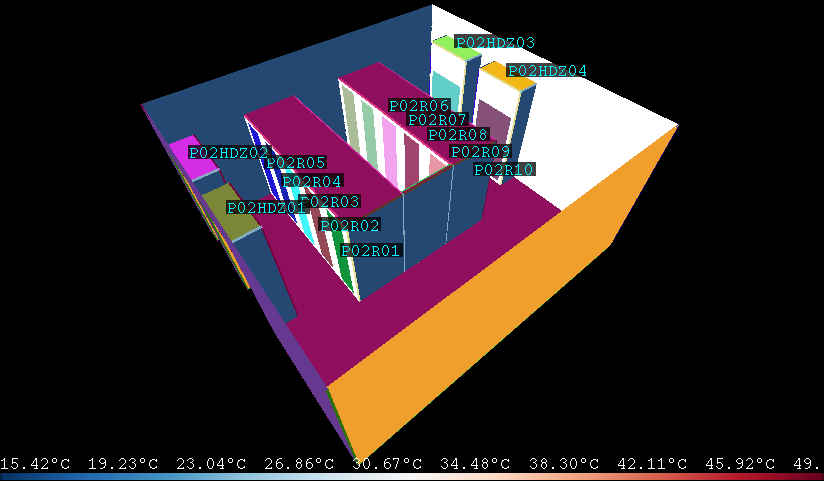
\includegraphics[width=\linewidth]{rafsine_pod2_voxel.jpg}
\end{center}
\caption{Geometry of data center module POD 2.}
\end{figure}
\end{frame}

%%%%%%%%%%%%%%%%%%%%%%%%%%%%%%%%%%%%%%%%%%%%%%%%%%%%%%%%%%%%%%%%%%%%%%%%
\begin{frame}{Data Center Model: Simulation}
\begin{figure}[ht]
\begin{center}
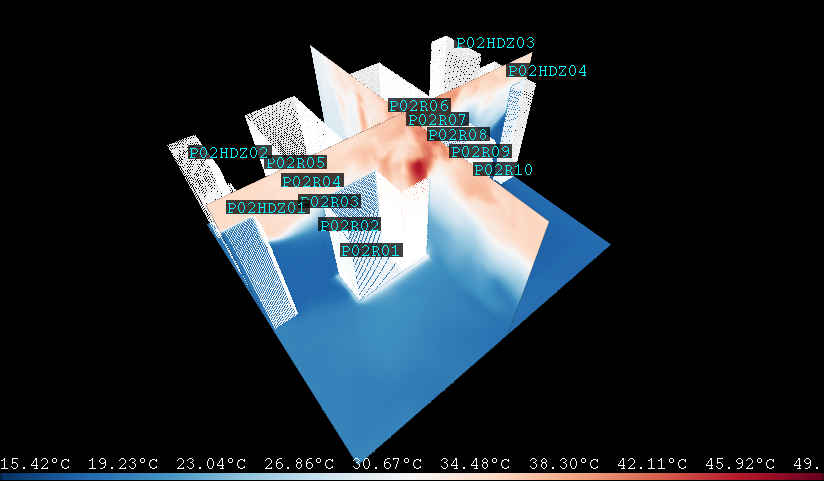
\includegraphics[width=\linewidth]{rafsine_pod2.jpg}
\end{center}
\caption{Simulating data center module POD 2.}
\end{figure}
\end{frame}

\section{Model Validation}
%%%%%%%%%%%%%%%%%%%%%%%%%%%%%%%%%%%%%%%%%%%%%%%%%%%%%%%%%%%%%%%%%%%%%%%%
\begin{frame}{Model Validation: CRACs}
\vspace{-1cm}
\begin{columns}[T] % align columns
\begin{column}{.6\textwidth}
	\begin{figure}[!htb]
	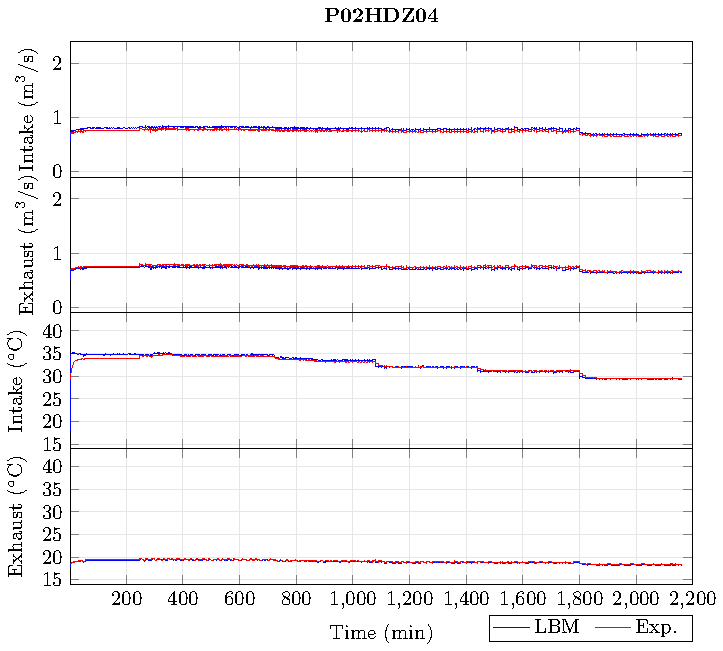
\includegraphics[width=\linewidth]{Plots/P02HDZ04_T.pdf}
	\end{figure}
\end{column}%
\hfill%<
\begin{column}{.6\textwidth}
	\begin{figure}[!htb]
	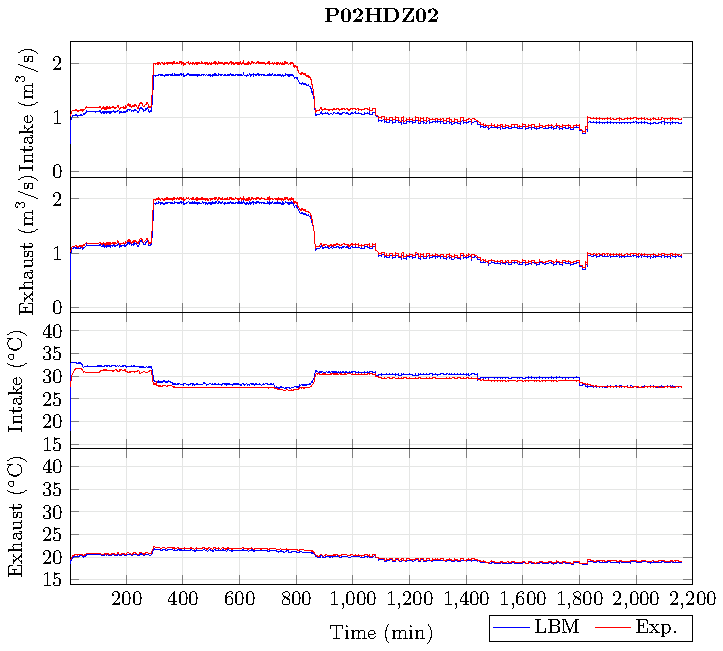
\includegraphics[width=\linewidth]{Plots/P02HDZ02_T.pdf}
	\end{figure}
\end{column}%
\end{columns}
\end{frame}

%%%%%%%%%%%%%%%%%%%%%%%%%%%%%%%%%%%%%%%%%%%%%%%%%%%%%%%%%%%%%%%%%%%%%%%%
\begin{frame}{Model Validation: Server Racks}
\begin{table}[h]
\caption{The RMS of the difference between simulated and experimental temperatures in \degree C, and volumetric flow rate in m$^3$/s at the inlets of the four CRAC units.}
\begin{center}
\resizebox{0.8\columnwidth}{!}{%
	\begin{tabular}{|l|m{1.7cm}|m{1.7cm}|m{1.7cm}|m{1.7cm}|}%
	\hline
	\bfseries CRAC & \bfseries \mbox{Inlet} temp.  & \bfseries \mbox{Exhaust} temp. & \bfseries \mbox{Inlet} flow & \bfseries \mbox{Exhaust} flow
	\csvreader[head to column names]{Plots/P02HDZX_TQ_rms.csv}{}% use head of csv as column names
	{\\\hline\crac&\Tin&\Tout&\Qin&\Qout}% specify your coloumns here
	\\\hline
	\end{tabular}
}
\end{center}
\label{tab:rms_crac_temps}
\end{table}
\end{frame}

%%%%%%%%%%%%%%%%%%%%%%%%%%%%%%%%%%%%%%%%%%%%%%%%%%%%%%%%%%%%%%%%%%%%%%%%
\begin{frame}{Model Validation: Server Racks}
	\begin{figure}[!htb]
	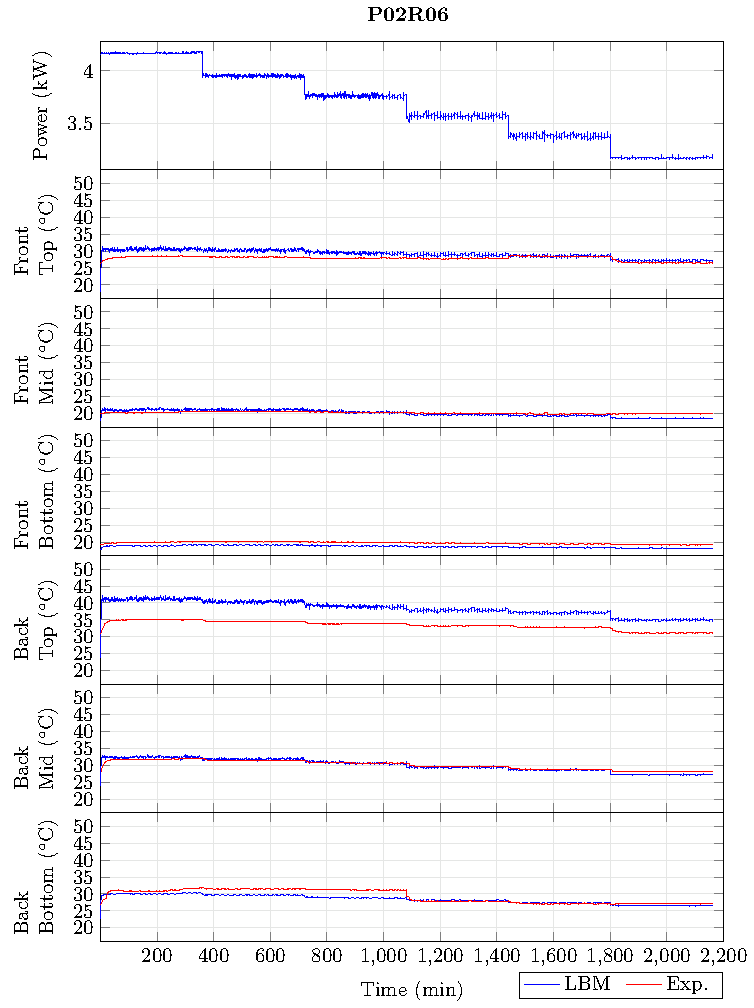
\includegraphics[width=0.58\linewidth]{Plots/P02R06_T.pdf}
	\end{figure}
\end{frame}

%%%%%%%%%%%%%%%%%%%%%%%%%%%%%%%%%%%%%%%%%%%%%%%%%%%%%%%%%%%%%%%%%%%%%%%%
\begin{frame}{Model Validation: Server Racks}
\begin{table}[h]
\caption{The RMS of the difference between simulated and experimental temperatures in \degree C at different positions on the server racks.}
\begin{center}
\resizebox{\columnwidth}{!}{%
	\begin{tabular}{|l|m{1.7cm}|m{1.7cm}|m{1.7cm}|m{1.7cm}|m{1.7cm}|m{1.7cm}|}%
	\hline
	\bfseries Rack & \bfseries Front Bottom & \bfseries Front Mid & \bfseries Front Top & \bfseries Back Bottom & \bfseries Back Mid & \bfseries Back Top
	\csvreader[head to column names]{Plots/P02RX_T_rms.csv}{}% use head of csv as column names
	{\\\hline\rack&\Tinb&\Tinm&\Tint&\Toutb&\Toutm&\Toutt}% specify your coloumns here
	\\\hline
	\end{tabular}
}
\end{center}
\label{tab:rms_rack_temps}
\end{table}
\end{frame}

%%%%%%%%%%%%%%%%%%%%%%%%%%%%%%%%%%%%%%%%%%%%%%%%%%%%%%%%%%%%%%%%%%%%%%%%
\begin{frame}{Model Validation: Sources of Error}

\begin{itemize}
\item Too coarse lattice resolution
\item Very simplified server rack geometry, server positioning
\item Temp sensor positions might be slightly off
\item Server fan speed and power consumption averaged for entire rack
\item Racks 1, 2, 3 missing fan speed data
\item Air flow rate could not be verified
\item Improve turbulence model
\end{itemize}

\end{frame}

\section{Future Work}
%%%%%%%%%%%%%%%%%%%%%%%%%%%%%%%%%%%%%%%%%%%%%%%%%%%%%%%%%%%%%%%%%%%%%%%%
\begin{frame}{Future Work}
\begin{itemize}
\item Model improvements
\item Better GUI, 3D CAD capability
\item Support MRT and Cascaded LBM
\item Multiple GPUs
\end{itemize}
\end{frame}


%%%%%%%%%%%%%%%%%%%%%%%%%%%%%%%%%%%%%%%%%%%%%%%%%%%%%%%%%%%%%%%%%%%%%%%%
\begin{frame}{Thanks for listening!}

\end{frame}

\end{document}
